\documentclass[]{article}
\usepackage{lmodern}
\usepackage{amssymb,amsmath}
\usepackage{ifxetex,ifluatex}
\usepackage{fixltx2e} % provides \textsubscript
\ifnum 0\ifxetex 1\fi\ifluatex 1\fi=0 % if pdftex
  \usepackage[T1]{fontenc}
  \usepackage[utf8]{inputenc}
\else % if luatex or xelatex
  \ifxetex
    \usepackage{mathspec}
  \else
    \usepackage{fontspec}
  \fi
  \defaultfontfeatures{Ligatures=TeX,Scale=MatchLowercase}
\fi
% use upquote if available, for straight quotes in verbatim environments
\IfFileExists{upquote.sty}{\usepackage{upquote}}{}
% use microtype if available
\IfFileExists{microtype.sty}{%
\usepackage{microtype}
\UseMicrotypeSet[protrusion]{basicmath} % disable protrusion for tt fonts
}{}
\usepackage[margin=1in]{geometry}
\usepackage{hyperref}
\hypersetup{unicode=true,
            pdftitle={Suffolk 2019},
            pdfborder={0 0 0},
            breaklinks=true}
\urlstyle{same}  % don't use monospace font for urls
\usepackage{color}
\usepackage{fancyvrb}
\newcommand{\VerbBar}{|}
\newcommand{\VERB}{\Verb[commandchars=\\\{\}]}
\DefineVerbatimEnvironment{Highlighting}{Verbatim}{commandchars=\\\{\}}
% Add ',fontsize=\small' for more characters per line
\usepackage{framed}
\definecolor{shadecolor}{RGB}{248,248,248}
\newenvironment{Shaded}{\begin{snugshade}}{\end{snugshade}}
\newcommand{\AlertTok}[1]{\textcolor[rgb]{0.94,0.16,0.16}{#1}}
\newcommand{\AnnotationTok}[1]{\textcolor[rgb]{0.56,0.35,0.01}{\textbf{\textit{#1}}}}
\newcommand{\AttributeTok}[1]{\textcolor[rgb]{0.77,0.63,0.00}{#1}}
\newcommand{\BaseNTok}[1]{\textcolor[rgb]{0.00,0.00,0.81}{#1}}
\newcommand{\BuiltInTok}[1]{#1}
\newcommand{\CharTok}[1]{\textcolor[rgb]{0.31,0.60,0.02}{#1}}
\newcommand{\CommentTok}[1]{\textcolor[rgb]{0.56,0.35,0.01}{\textit{#1}}}
\newcommand{\CommentVarTok}[1]{\textcolor[rgb]{0.56,0.35,0.01}{\textbf{\textit{#1}}}}
\newcommand{\ConstantTok}[1]{\textcolor[rgb]{0.00,0.00,0.00}{#1}}
\newcommand{\ControlFlowTok}[1]{\textcolor[rgb]{0.13,0.29,0.53}{\textbf{#1}}}
\newcommand{\DataTypeTok}[1]{\textcolor[rgb]{0.13,0.29,0.53}{#1}}
\newcommand{\DecValTok}[1]{\textcolor[rgb]{0.00,0.00,0.81}{#1}}
\newcommand{\DocumentationTok}[1]{\textcolor[rgb]{0.56,0.35,0.01}{\textbf{\textit{#1}}}}
\newcommand{\ErrorTok}[1]{\textcolor[rgb]{0.64,0.00,0.00}{\textbf{#1}}}
\newcommand{\ExtensionTok}[1]{#1}
\newcommand{\FloatTok}[1]{\textcolor[rgb]{0.00,0.00,0.81}{#1}}
\newcommand{\FunctionTok}[1]{\textcolor[rgb]{0.00,0.00,0.00}{#1}}
\newcommand{\ImportTok}[1]{#1}
\newcommand{\InformationTok}[1]{\textcolor[rgb]{0.56,0.35,0.01}{\textbf{\textit{#1}}}}
\newcommand{\KeywordTok}[1]{\textcolor[rgb]{0.13,0.29,0.53}{\textbf{#1}}}
\newcommand{\NormalTok}[1]{#1}
\newcommand{\OperatorTok}[1]{\textcolor[rgb]{0.81,0.36,0.00}{\textbf{#1}}}
\newcommand{\OtherTok}[1]{\textcolor[rgb]{0.56,0.35,0.01}{#1}}
\newcommand{\PreprocessorTok}[1]{\textcolor[rgb]{0.56,0.35,0.01}{\textit{#1}}}
\newcommand{\RegionMarkerTok}[1]{#1}
\newcommand{\SpecialCharTok}[1]{\textcolor[rgb]{0.00,0.00,0.00}{#1}}
\newcommand{\SpecialStringTok}[1]{\textcolor[rgb]{0.31,0.60,0.02}{#1}}
\newcommand{\StringTok}[1]{\textcolor[rgb]{0.31,0.60,0.02}{#1}}
\newcommand{\VariableTok}[1]{\textcolor[rgb]{0.00,0.00,0.00}{#1}}
\newcommand{\VerbatimStringTok}[1]{\textcolor[rgb]{0.31,0.60,0.02}{#1}}
\newcommand{\WarningTok}[1]{\textcolor[rgb]{0.56,0.35,0.01}{\textbf{\textit{#1}}}}
\usepackage{longtable,booktabs}
\usepackage{graphicx,grffile}
\makeatletter
\def\maxwidth{\ifdim\Gin@nat@width>\linewidth\linewidth\else\Gin@nat@width\fi}
\def\maxheight{\ifdim\Gin@nat@height>\textheight\textheight\else\Gin@nat@height\fi}
\makeatother
% Scale images if necessary, so that they will not overflow the page
% margins by default, and it is still possible to overwrite the defaults
% using explicit options in \includegraphics[width, height, ...]{}
\setkeys{Gin}{width=\maxwidth,height=\maxheight,keepaspectratio}
\IfFileExists{parskip.sty}{%
\usepackage{parskip}
}{% else
\setlength{\parindent}{0pt}
\setlength{\parskip}{6pt plus 2pt minus 1pt}
}
\setlength{\emergencystretch}{3em}  % prevent overfull lines
\providecommand{\tightlist}{%
  \setlength{\itemsep}{0pt}\setlength{\parskip}{0pt}}
\setcounter{secnumdepth}{5}
% Redefines (sub)paragraphs to behave more like sections
\ifx\paragraph\undefined\else
\let\oldparagraph\paragraph
\renewcommand{\paragraph}[1]{\oldparagraph{#1}\mbox{}}
\fi
\ifx\subparagraph\undefined\else
\let\oldsubparagraph\subparagraph
\renewcommand{\subparagraph}[1]{\oldsubparagraph{#1}\mbox{}}
\fi

%%% Use protect on footnotes to avoid problems with footnotes in titles
\let\rmarkdownfootnote\footnote%
\def\footnote{\protect\rmarkdownfootnote}

%%% Change title format to be more compact
\usepackage{titling}

% Create subtitle command for use in maketitle
\providecommand{\subtitle}[1]{
  \posttitle{
    \begin{center}\large#1\end{center}
    }
}

\setlength{\droptitle}{-2em}

  \title{Suffolk 2019}
    \pretitle{\vspace{\droptitle}\centering\huge}
  \posttitle{\par}
    \author{}
    \preauthor{}\postauthor{}
    \date{}
    \predate{}\postdate{}
  

\begin{document}
\maketitle

{
\setcounter{tocdepth}{2}
\tableofcontents
}
\hypertarget{about-this-course}{%
\section*{About this course}\label{about-this-course}}
\addcontentsline{toc}{section}{About this course}

This course is an introduction R, RStudio and statistics. Our primary aims are to get comfortable working with R and to be able to prepare, manipulate, analyse and visualise data.

\begin{center}\rule{0.5\linewidth}{\linethickness}\end{center}

Slides day 1

\hypertarget{introduction-to-r-and-rstudio}{%
\section{Introduction to R and RStudio}\label{introduction-to-r-and-rstudio}}

\hypertarget{learning-objectives}{%
\subsection{Learning objectives}\label{learning-objectives}}

In this session, we will have a look at R and RStudio. We will interact with both and use the various components of RStudio.

\hypertarget{what-is-r}{%
\subsubsection{What is R?}\label{what-is-r}}

R is an environment for statistical computing and graphics. RStudio is an editor or integrated development environment (IDE) that makes working with R much more comfortable.

To install R and RStudio on your computer, download both from the following sources:

\begin{itemize}
\tightlist
\item
  Download R from \href{https://cran.r-project.org}{The Comprehensive R Archive Network (CRAN)}
\item
  Download RStudio from \href{https://www.rstudio.com}{RStudio.com}
\end{itemize}

Keep both R and RStudio up to date. That means go online and check for newer versions. In case there are new versions, download those and re-install.

\hypertarget{rstudio}{%
\subsubsection{RStudio}\label{rstudio}}

Let's get acquainted with R. When you start RStudio for the first time, you'll see three panes:

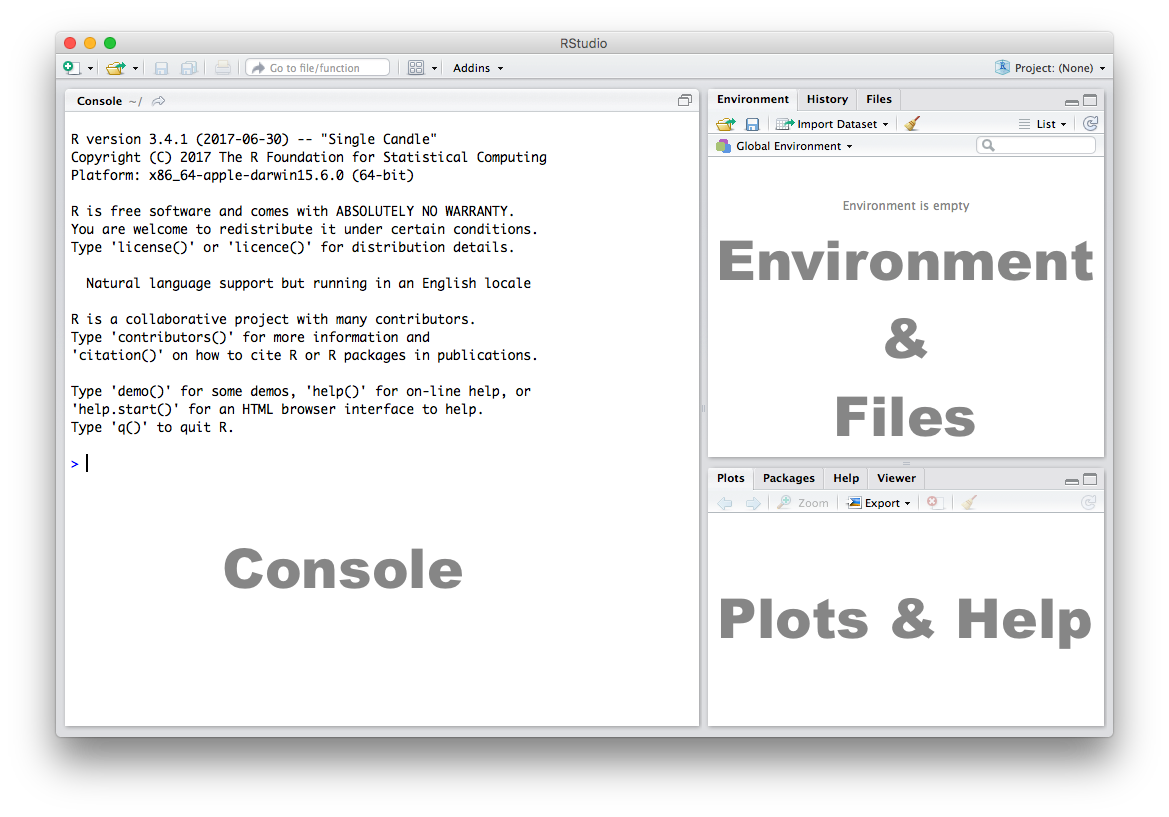
\includegraphics{./img/rstudio_default.png}

\hypertarget{console}{%
\subsubsection{Console}\label{console}}

The Console in RStudio is the simplest way to interact with R. You can type some code at the Console and when you press ENTER, R will run that code. Depending on what you type, you may see some output in the Console or if you make a mistake, you may get a warning or an error message.

Let's familiarize ourselves with the console by using R as a simple calculator:

\begin{Shaded}
\begin{Highlighting}[]
\DecValTok{2} \OperatorTok{+}\StringTok{ }\DecValTok{4}
\end{Highlighting}
\end{Shaded}

\begin{verbatim}
[1] 6
\end{verbatim}

Now that we know how to use the \texttt{+} sign for addition, let's try some other mathematical operations such as subtraction (\texttt{-}), multiplication (\texttt{*}), and division (\texttt{/}).

\begin{Shaded}
\begin{Highlighting}[]
\DecValTok{10} \OperatorTok{-}\StringTok{ }\DecValTok{4}
\end{Highlighting}
\end{Shaded}

\begin{verbatim}
[1] 6
\end{verbatim}

\begin{Shaded}
\begin{Highlighting}[]
\DecValTok{5} \OperatorTok{*}\StringTok{ }\DecValTok{3}
\end{Highlighting}
\end{Shaded}

\begin{verbatim}
[1] 15
\end{verbatim}

\begin{Shaded}
\begin{Highlighting}[]
\DecValTok{7} \OperatorTok{/}\StringTok{ }\DecValTok{2}
\end{Highlighting}
\end{Shaded}

\begin{verbatim}
[1] 3.5
\end{verbatim}

\begin{longtable}[]{@{}ll@{}}
\toprule
\endhead
\begin{minipage}[t]{0.69\columnwidth}\raggedright
You can use the cursor or arrow keys on your keyboard to edit your code at the console:- Use the UP and DOWN keys to re-run something without typing it again- Use the LEFT and RIGHT keys to edit\strut
\end{minipage} & \begin{minipage}[t]{0.25\columnwidth}\raggedright
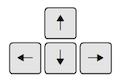
\includegraphics{./img/rstudio_cursorkeys.png}\strut
\end{minipage}\tabularnewline
\bottomrule
\end{longtable}

Take a few minutes to play around at the console and try different things out. Don't worry if you make a mistake, you can't break anything easily!

\hypertarget{scripts}{%
\subsubsection{Scripts}\label{scripts}}

The Console is great for simple tasks but if you're working on a project you would mostly likely want to save your work in some sort of a document or a file. Scripts in R are just plain text files that contain R code. You can edit a script just like you would edit a file in any word processing or note-taking application.

Create a new script using the menu or the toolbar button as shown below.

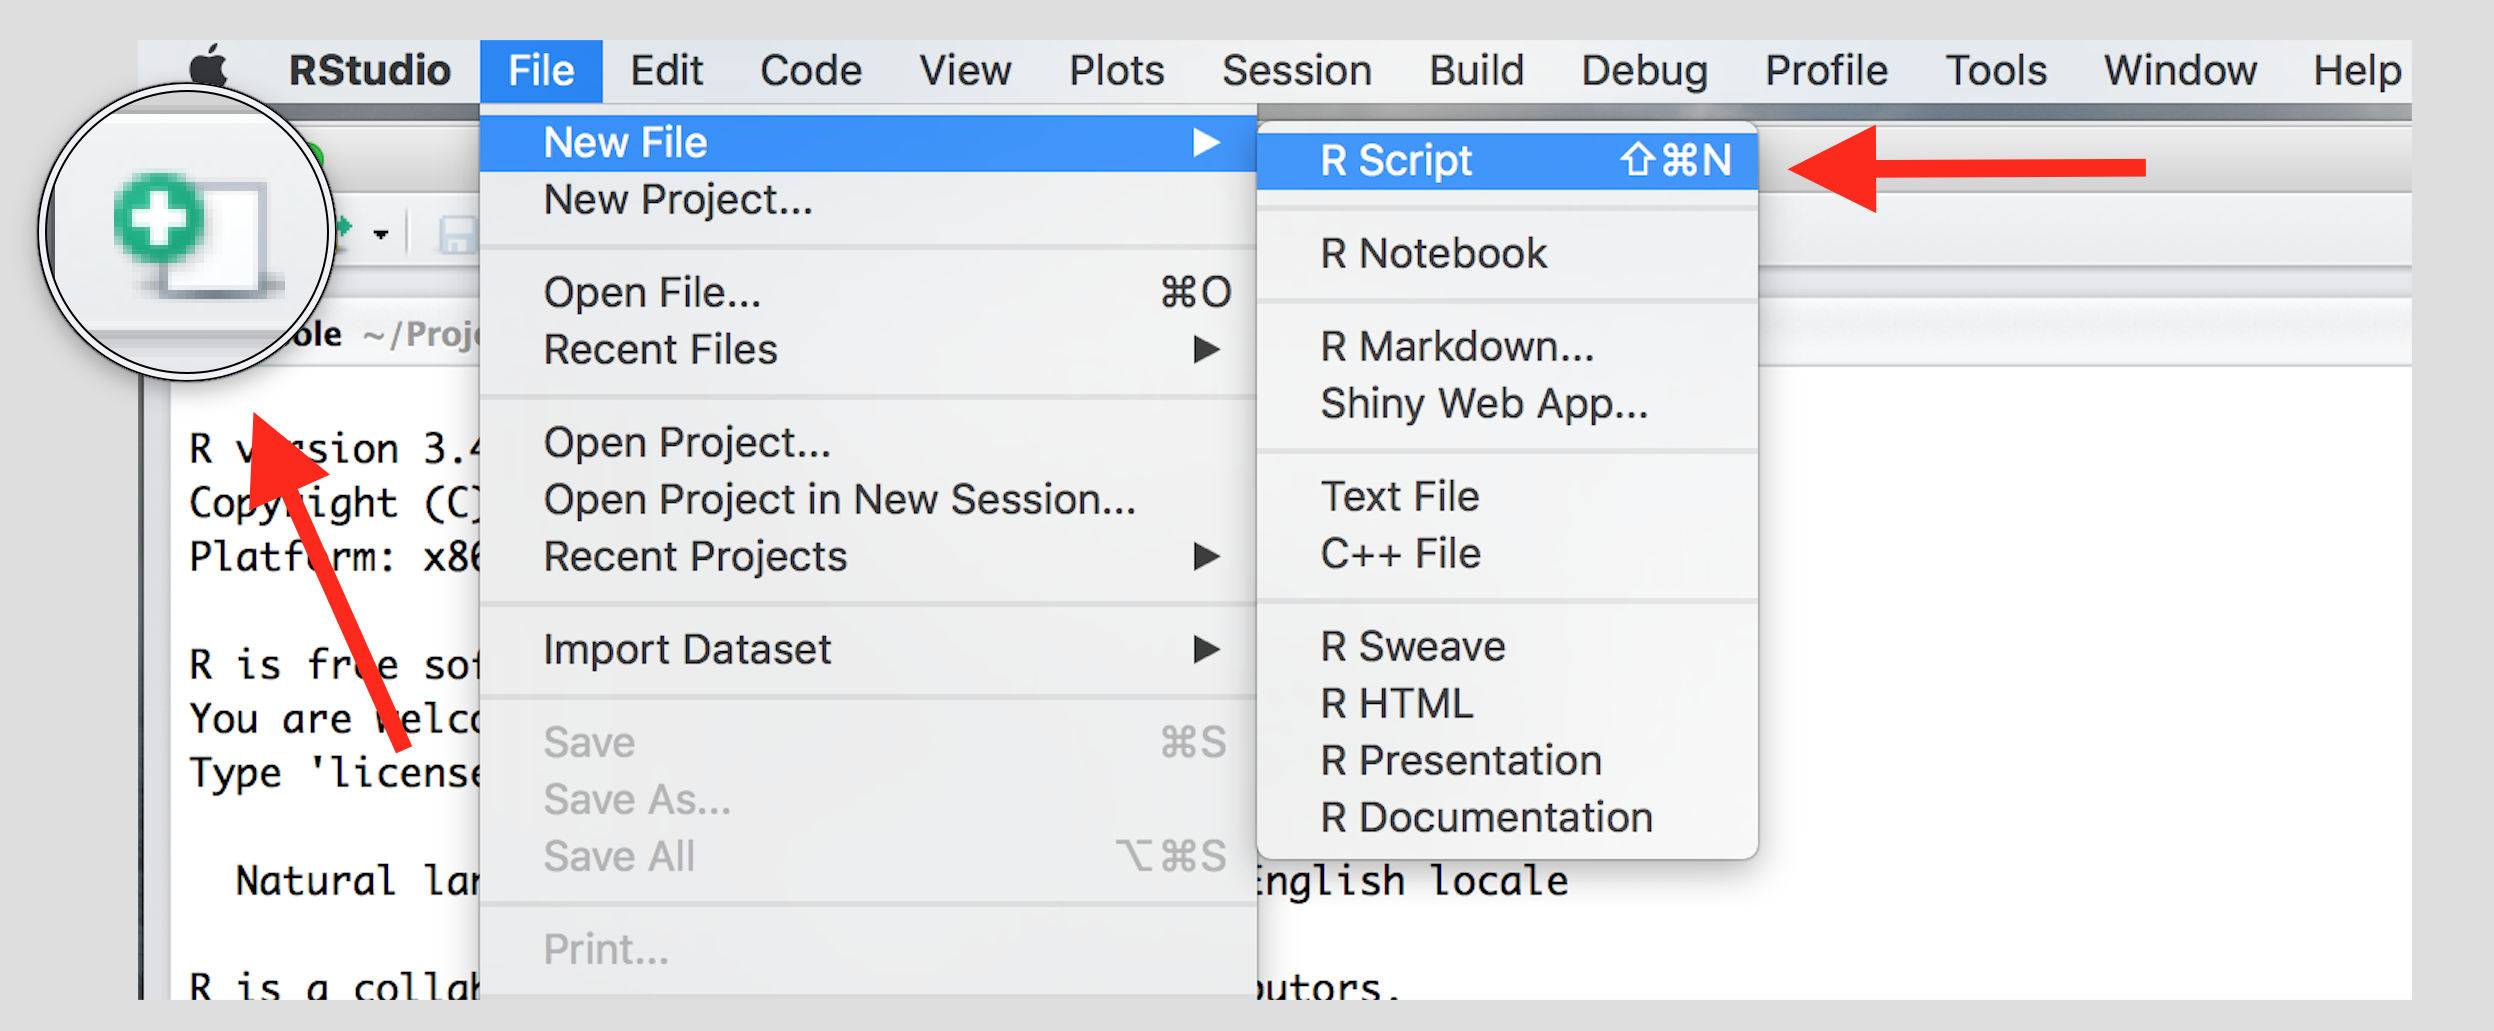
\includegraphics{./img/rstudio_newfile.png}

Once you've created a script, it is generally a good idea to give it a meaningful name and save it immediately. For our first session save your script as \textbf{seminar1.R}

\begin{longtable}[]{@{}ll@{}}
\toprule
\endhead
\begin{minipage}[t]{0.52\columnwidth}\raggedright
Familiarize yourself with the script window in RStudio, and especially the two buttons labeled \textbf{Run} and \textbf{Source}\strut
\end{minipage} & \begin{minipage}[t]{0.42\columnwidth}\raggedright
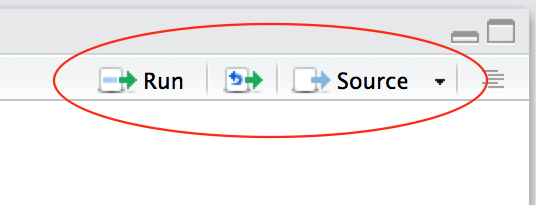
\includegraphics{./img/rstudio_script.png}\strut
\end{minipage}\tabularnewline
\bottomrule
\end{longtable}

There are a few different ways to run your code from a script.

\begin{longtable}[]{@{}ll@{}}
\toprule
\endhead
\begin{minipage}[t]{0.23\columnwidth}\raggedright
One line at a time\strut
\end{minipage} & \begin{minipage}[t]{0.71\columnwidth}\raggedright
Place the cursor on the line you want to run and hit CTRL-ENTER or use the \textbf{Run} button\strut
\end{minipage}\tabularnewline
\begin{minipage}[t]{0.23\columnwidth}\raggedright
Multiple lines\strut
\end{minipage} & \begin{minipage}[t]{0.71\columnwidth}\raggedright
Select the lines you want to run and hit CTRL-ENTER or use the \textbf{Run} button\strut
\end{minipage}\tabularnewline
\begin{minipage}[t]{0.23\columnwidth}\raggedright
Entire script\strut
\end{minipage} & \begin{minipage}[t]{0.71\columnwidth}\raggedright
Use the \textbf{Source} button\strut
\end{minipage}\tabularnewline
\bottomrule
\end{longtable}

\hypertarget{r-syntax-data-structures-and-types}{%
\section{R-syntax, data structures and types}\label{r-syntax-data-structures-and-types}}

\hypertarget{seminar}{%
\subsection{Seminar}\label{seminar}}

In this session we introduce R-syntax, and data types.

\hypertarget{functions}{%
\subsubsection{Functions}\label{functions}}

Functions are a set of instructions that carry out a specific task. Functions often require some input and generate some output. For example, instead of using the \texttt{+} operator for addition, we can use the \texttt{sum} function to add two or more numbers.

\begin{Shaded}
\begin{Highlighting}[]
\KeywordTok{sum}\NormalTok{(}\DecValTok{1}\NormalTok{, }\DecValTok{4}\NormalTok{, }\DecValTok{10}\NormalTok{)}
\end{Highlighting}
\end{Shaded}

\begin{verbatim}
[1] 15
\end{verbatim}

In the example above, \texttt{1,\ 4,\ 10} are the inputs and 15 is the output. A function always requires the use of parenthesis or round brackets \texttt{()}. Inputs to the function are called \textbf{arguments} and go inside the brackets. The output of a function is displayed on the screen but we can also have the option of saving the result of the output. More on this later.

\hypertarget{getting-help}{%
\subsubsection{Getting Help}\label{getting-help}}

Another useful function in R is \texttt{help} which we can use to display online documentation. For example, if we wanted to know how to use the \texttt{sum} function, we could type \texttt{help(sum)} and look at the online documentation.

\begin{Shaded}
\begin{Highlighting}[]
\KeywordTok{help}\NormalTok{(sum)}
\end{Highlighting}
\end{Shaded}

The question mark \texttt{?} can also be used as a shortcut to access online help.

\begin{Shaded}
\begin{Highlighting}[]
\NormalTok{?sum}
\end{Highlighting}
\end{Shaded}

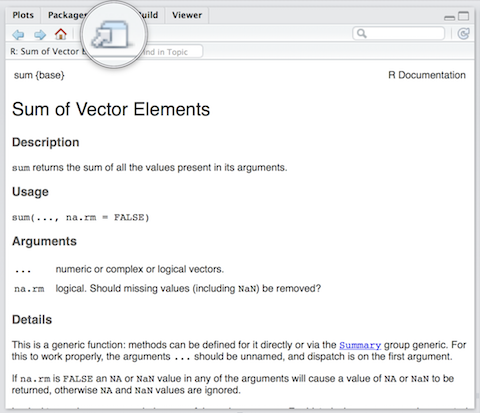
\includegraphics{./img/rstudio_help.png}

Use the toolbar button shown in the picture above to expand and display the help in a new window.

Help pages for functions in R follow a consistent layout generally include these sections:

\begin{longtable}[]{@{}ll@{}}
\toprule
\endhead
Description & A brief description of the function\tabularnewline
Usage & The complete syntax or grammar including all arguments (inputs)\tabularnewline
Arguments & Explanation of each argument\tabularnewline
Details & Any relevant details about the function and its arguments\tabularnewline
Value & The output value of the function\tabularnewline
Examples & Example of how to use the function\tabularnewline
\bottomrule
\end{longtable}

\hypertarget{the-assignment-operator}{%
\subsubsection{The Assignment Operator}\label{the-assignment-operator}}

Now we know how to provide inputs to a function using parenthesis or round brackets \texttt{()}, but what about the output of a function?

We use the assignment operator \textbf{\texttt{\textless{}-}} for creating or updating objects. If we wanted to save the result of adding \texttt{sum(1,\ 4,\ 10)}, we would do the following:

\begin{Shaded}
\begin{Highlighting}[]
\NormalTok{myresult <-}\StringTok{ }\KeywordTok{sum}\NormalTok{(}\DecValTok{1}\NormalTok{, }\DecValTok{4}\NormalTok{, }\DecValTok{10}\NormalTok{)}
\end{Highlighting}
\end{Shaded}

The line above creates a new object called \texttt{myresult} in our environment and saves the result of the \texttt{sum(1,\ 4,\ 10)} in it. To see what's in \texttt{myresult}, just type it at the console:

\begin{Shaded}
\begin{Highlighting}[]
\NormalTok{myresult}
\end{Highlighting}
\end{Shaded}

\begin{verbatim}
[1] 15
\end{verbatim}

Take a look at the \textbf{Environment} pane in RStudio and you'll see \texttt{myresult} there.

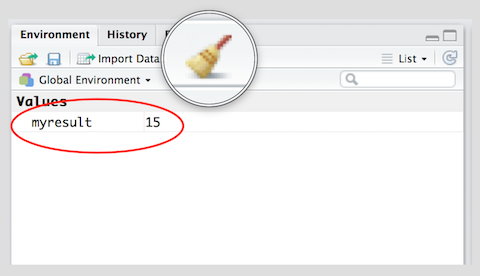
\includegraphics{./img/rstudio_env.png}

To delete all objects from the environment, you can use the \textbf{broom} button as shown in the picture above.

We called our object \texttt{myresult} but we can call it anything as long as we follow a few simple rules. Object names can contain upper or lower case letters (\texttt{A-Z}, \texttt{a-z}), numbers (\texttt{0-9}), underscores (\texttt{\_}) or a dot (\texttt{.}) but all object names must start with a letter. Choose names that are descriptive and easy to type.

\begin{longtable}[]{@{}ll@{}}
\toprule
Good Object Names & Bad Object Names\tabularnewline
\midrule
\endhead
result & a\tabularnewline
myresult & x1\tabularnewline
my.result & this.name.is.just.too.long\tabularnewline
my\_result &\tabularnewline
data1 &\tabularnewline
\bottomrule
\end{longtable}

\hypertarget{vectors-and-subsetting}{%
\subsubsection{Vectors and subsetting}\label{vectors-and-subsetting}}

A vector is one dimensional. It can contain one element in which case it is also called a scalar or many elements. We can add and multiply vectors. Think of a vector as a row or column in your excel spreadsheet.

To create a vector, we use the \texttt{c()} function, where c stands for collect. We start by creating a numeric vector.

\begin{Shaded}
\begin{Highlighting}[]
\NormalTok{vec1 <-}\StringTok{ }\KeywordTok{c}\NormalTok{(}\DecValTok{10}\NormalTok{, }\DecValTok{47}\NormalTok{, }\DecValTok{99}\NormalTok{, }\DecValTok{34}\NormalTok{, }\DecValTok{21}\NormalTok{)}
\end{Highlighting}
\end{Shaded}

Creating a character vector works in the same way. We need to use quotation marks to indicate that the data type is textual data.

\begin{Shaded}
\begin{Highlighting}[]
\NormalTok{vec2 <-}\StringTok{ }\KeywordTok{c}\NormalTok{(}\StringTok{"Emilia"}\NormalTok{, }\StringTok{"Martin"}\NormalTok{, }\StringTok{"Agatha"}\NormalTok{, }\StringTok{"James"}\NormalTok{, }\StringTok{"Luke"}\NormalTok{, }\StringTok{"Jacques"}\NormalTok{)}
\end{Highlighting}
\end{Shaded}

Let's see how many elements our vector contains using the \texttt{length()} function.

\begin{Shaded}
\begin{Highlighting}[]
\KeywordTok{length}\NormalTok{(vec1)}
\end{Highlighting}
\end{Shaded}

\begin{verbatim}
[1] 5
\end{verbatim}

\begin{Shaded}
\begin{Highlighting}[]
\KeywordTok{length}\NormalTok{(vec2)}
\end{Highlighting}
\end{Shaded}

\begin{verbatim}
[1] 6
\end{verbatim}

We need one coordinate to identify a unique element in a vector. For instance, we may be interested in the first element of the vector only. We use square brackets \texttt{{[}{]}} to access a specific element. The number in square brackets is the vector element that we wish to see.

\begin{Shaded}
\begin{Highlighting}[]
\NormalTok{vec1[}\DecValTok{1}\NormalTok{]}
\end{Highlighting}
\end{Shaded}

\begin{verbatim}
[1] 10
\end{verbatim}

To access all elements except the first element, we use the \texttt{-} operator

\begin{Shaded}
\begin{Highlighting}[]
\NormalTok{vec1[}\OperatorTok{-}\DecValTok{1}\NormalTok{]}
\end{Highlighting}
\end{Shaded}

\begin{verbatim}
[1] 47 99 34 21
\end{verbatim}

We can access elements 2 to 4 by using the colon \texttt{:} operator.

\begin{Shaded}
\begin{Highlighting}[]
\NormalTok{vec1[}\DecValTok{2}\OperatorTok{:}\DecValTok{4}\NormalTok{]}
\end{Highlighting}
\end{Shaded}

\begin{verbatim}
[1] 47 99 34
\end{verbatim}

We can access non-adjacent elements bu using the collect function \texttt{c()}.

\begin{Shaded}
\begin{Highlighting}[]
\NormalTok{vec1[}\KeywordTok{c}\NormalTok{(}\DecValTok{2}\NormalTok{,}\DecValTok{5}\NormalTok{)]}
\end{Highlighting}
\end{Shaded}

\begin{verbatim}
[1] 47 21
\end{verbatim}

Finally, we combine the \texttt{length()} function with the square brackets to access the last element in our vector.

\begin{Shaded}
\begin{Highlighting}[]
\NormalTok{vec1[ }\KeywordTok{length}\NormalTok{(vec1) ]}
\end{Highlighting}
\end{Shaded}

\begin{verbatim}
[1] 21
\end{verbatim}

\hypertarget{matrices}{%
\subsubsection{Matrices}\label{matrices}}

A matrix has two dimensions and stores data of the same type, e.g.~numbers or text but never both. A matrix is always rectangular. Think of it as your excel spreadsheet - essentially, it is a data table.

We create a matrix using the \texttt{matrix()} function. We need to provide the following arguments:

\begin{Shaded}
\begin{Highlighting}[]
\NormalTok{mat1 <-}\StringTok{ }\KeywordTok{matrix}\NormalTok{(}
  \DataTypeTok{data =} \KeywordTok{c}\NormalTok{(}\DecValTok{99}\NormalTok{, }\DecValTok{17}\NormalTok{, }\DecValTok{19}\NormalTok{, }\DecValTok{49}\NormalTok{, }\DecValTok{88}\NormalTok{, }\DecValTok{54}\NormalTok{),}
  \DataTypeTok{nrow =} \DecValTok{2}\NormalTok{,}
  \DataTypeTok{ncol =} \DecValTok{3}\NormalTok{,}
  \DataTypeTok{byrow =} \OtherTok{TRUE}
\NormalTok{)}
\end{Highlighting}
\end{Shaded}

\begin{longtable}[]{@{}ll@{}}
\toprule
Argument & Description\tabularnewline
\midrule
\endhead
data & the data in the matrix\tabularnewline
nrow & number of rows\tabularnewline
ncol & number of columns\tabularnewline
byrow & TRUE = matrix is filled rowwise\tabularnewline
\bottomrule
\end{longtable}

To display the matrix, we simply call the object by its name (in this case mat1).

\begin{Shaded}
\begin{Highlighting}[]
\NormalTok{mat1}
\end{Highlighting}
\end{Shaded}

\begin{verbatim}
     [,1] [,2] [,3]
[1,]   99   17   19
[2,]   49   88   54
\end{verbatim}

To access a unique element in a matrix, we need 2 coordinates. First, a row coordinate and second, a column coordinate. We use square brackets and separate the coordinates with a comma \texttt{{[}\ ,\ {]}}. The row coordinate goes before the comma and the column coordinate after.

We can access the the second row and third column like so:

\begin{Shaded}
\begin{Highlighting}[]
\NormalTok{mat1[}\DecValTok{2}\NormalTok{, }\DecValTok{3}\NormalTok{]}
\end{Highlighting}
\end{Shaded}

\begin{verbatim}
[1] 54
\end{verbatim}

To display an entire column, we specify the column we want to display and leave the row coordinate empty like so:

\begin{Shaded}
\begin{Highlighting}[]
\CommentTok{# display the 2nd column}
\NormalTok{mat1[ , }\DecValTok{2}\NormalTok{]}
\end{Highlighting}
\end{Shaded}

\begin{verbatim}
[1] 17 88
\end{verbatim}

Similarly, to display the entire second row, we specify the row coordinate but leave the column coordinate empty.

\begin{Shaded}
\begin{Highlighting}[]
\NormalTok{mat1[}\DecValTok{2}\NormalTok{, ]}
\end{Highlighting}
\end{Shaded}

\begin{verbatim}
[1] 49 88 54
\end{verbatim}

\hypertarget{arrays}{%
\subsubsection{Arrays}\label{arrays}}

Arrays are similar to matrices but can contain more dimensions. You can think of an array as stacking multiple matrices. Generally, we refer to the rows, columns and layers in array. Let's create an array with 2 rows, 3 columns and 4 layers using the \texttt{array()} function.

\begin{Shaded}
\begin{Highlighting}[]
\NormalTok{arr1 <-}\StringTok{ }\KeywordTok{array}\NormalTok{(}
  \DataTypeTok{data =} \KeywordTok{c}\NormalTok{(}\DecValTok{1}\OperatorTok{:}\DecValTok{24}\NormalTok{),}
  \DataTypeTok{dim =} \KeywordTok{c}\NormalTok{(}\DecValTok{2}\NormalTok{, }\DecValTok{3}\NormalTok{, }\DecValTok{4}\NormalTok{)}
\NormalTok{)}
\end{Highlighting}
\end{Shaded}

To display the object, we call it by its name.

\begin{Shaded}
\begin{Highlighting}[]
\NormalTok{arr1}
\end{Highlighting}
\end{Shaded}

\begin{verbatim}
, , 1

     [,1] [,2] [,3]
[1,]    1    3    5
[2,]    2    4    6

, , 2

     [,1] [,2] [,3]
[1,]    7    9   11
[2,]    8   10   12

, , 3

     [,1] [,2] [,3]
[1,]   13   15   17
[2,]   14   16   18

, , 4

     [,1] [,2] [,3]
[1,]   19   21   23
[2,]   20   22   24
\end{verbatim}

We can subset an array using the square brackets \texttt{{[}{]}}. To access a single element we need as many coordinates as our object has dimensions. Let's check the number of dimensions in our object first.

\begin{Shaded}
\begin{Highlighting}[]
\KeywordTok{dim}\NormalTok{(arr1)}
\end{Highlighting}
\end{Shaded}

\begin{verbatim}
[1] 2 3 4
\end{verbatim}

The \texttt{dim()} function informs us that we have 3 dimensions. The first is of length 2, the second of length 3 and the fourth of length 4.

Access the second column of the third layer on your own.

\begin{Shaded}
\begin{Highlighting}[]
\NormalTok{arr1[ , }\DecValTok{2}\NormalTok{, }\DecValTok{3}\NormalTok{] }
\end{Highlighting}
\end{Shaded}

\begin{verbatim}
[1] 15 16
\end{verbatim}

\hypertarget{data-import-from-csv-txt-and-excel}{%
\section{Data import (from csv, txt, and excel)}\label{data-import-from-csv-txt-and-excel}}

\hypertarget{seminar-1}{%
\subsection{Seminar}\label{seminar-1}}

In this section, we will load data in csv, txt, excel and R format. We will learn how to check and set our working directory.

\hypertarget{setting-up}{%
\subsubsection{Setting up}\label{setting-up}}

We set our working directory. R operates in specific directory (folder) on our computer. We create a folder on where we save our scripts. We name the folder \texttt{suffolk2019}. Let's create the folder on our computers now (in finder on Mac and explorer on Windows).

Now, we set our working directory to the folder, we just created like so:

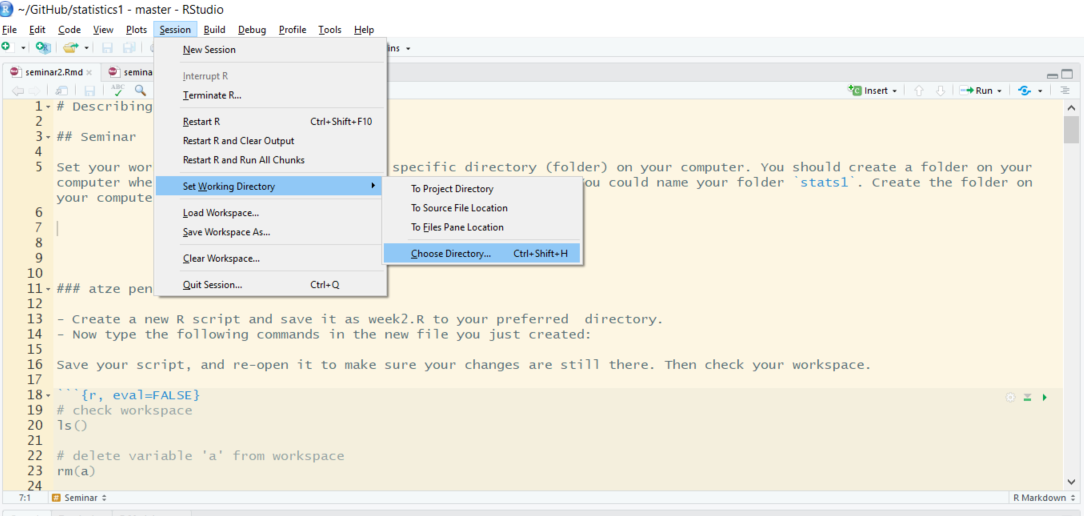
\includegraphics{./img/setwdir.png}

Create a new R script and save it as day1.R to your \texttt{suffolk2019} directory.

At the beginning of each new script, we want to clear the workspace. The workspace is stored in working memory on our computer. If we do not clear it for a new script, it becomes too full over time. Our computer will slow down and it will become difficult for us to know which objects are stored in working memory.

We check the contents of our workspace like so:

\begin{Shaded}
\begin{Highlighting}[]
\CommentTok{# check workspace}
\KeywordTok{ls}\NormalTok{()}
\end{Highlighting}
\end{Shaded}

To remove a specific object, we use the \texttt{rm()} function which stands for remove. Within the round brackets, we put the name of the object we want to remove. We could remove the object \texttt{a} like so:

\begin{Shaded}
\begin{Highlighting}[]
\CommentTok{# delete variable 'a' from workspace}
\KeywordTok{rm}\NormalTok{(a)}
\end{Highlighting}
\end{Shaded}

At the beginning of each script, we should always clear the entire workspace. We can do so in the following way:

\begin{Shaded}
\begin{Highlighting}[]
\CommentTok{# delete everything from workspace}
\KeywordTok{rm}\NormalTok{( }\DataTypeTok{list =} \KeywordTok{ls}\NormalTok{() )}
\end{Highlighting}
\end{Shaded}

You can also clear text from the console window. To do so press Crtl+l on Winowds or Command+l on Mac.

\hypertarget{loading-data}{%
\subsubsection{Loading data}\label{loading-data}}

Data comes in different file formats such as \texttt{.txt}, \texttt{.csv}, \texttt{.xlsx}, \texttt{.RData}, \texttt{.dta} and many more. To know the file type of a file right click on it and view preferences (in Windows explorer or Mac finder).

R can load files coming in many different file formats. To find out how to import a file coming in a specific format, it is usually a good idea to the google ``R load file\_format''.

\hypertarget{importing-a-dataset-in-.csv-format}{%
\subsubsection{\texorpdfstring{Importing a dataset in \texttt{.csv} format}{Importing a dataset in .csv format}}\label{importing-a-dataset-in-.csv-format}}

One of the most common file types is \texttt{.csv} which means comma separated values. Columns are separated by commas and rows by line breaks.

The dataset's name is ``non\_western\_immigrants.csv''. To load it, we use the \texttt{read.csv()} function.

\begin{Shaded}
\begin{Highlighting}[]
\NormalTok{dat1 <-}\StringTok{ }\KeywordTok{read.csv}\NormalTok{(}\StringTok{"non_western_immigrants.csv"}\NormalTok{)}
\end{Highlighting}
\end{Shaded}

\hypertarget{importing-a-dataset-in-excel-xlsx-format}{%
\subsubsection{Importing a dataset in Excel (xlsx) format}\label{importing-a-dataset-in-excel-xlsx-format}}

Another common file format is Microsoft's Excel \texttt{xlsx} format. We will load a dataset in this format now. To do so, we will need to install a package first. Packages are additional functions that we can add to R. A package is like an app on our phones.

We install the \texttt{readxl} package using \texttt{install.packages("readxl")}.

\begin{Shaded}
\begin{Highlighting}[]
\KeywordTok{install.packages}\NormalTok{(}\StringTok{"readxl"}\NormalTok{)}
\end{Highlighting}
\end{Shaded}

We only need to install a package once. It does not hurt to do it more often though, because every time we install, it will install the most recent version of the package.

Once a package is installed, we need to load it using the \texttt{library()} function.

\begin{Shaded}
\begin{Highlighting}[]
\KeywordTok{library}\NormalTok{(readxl)}
\end{Highlighting}
\end{Shaded}

To load the excel file, we can now use the \texttt{read\_excel()} function that is included in the \texttt{readxl} library. We need to provide the following arguments to the function:

\begin{longtable}[]{@{}ll@{}}
\toprule
Argument & Description\tabularnewline
\midrule
\endhead
path & Filename of excel sheet\tabularnewline
sheet & Sheet number to import\tabularnewline
\bottomrule
\end{longtable}

Now, let's load the file:

\begin{Shaded}
\begin{Highlighting}[]
\NormalTok{dat2 <-}\StringTok{ }\KeywordTok{read_excel}\NormalTok{(}\StringTok{"non_western_immigrants.xlsx"}\NormalTok{, }\DataTypeTok{sheet =} \DecValTok{1}\NormalTok{)}
\end{Highlighting}
\end{Shaded}

\hypertarget{importing-a-dataset-in-rdata-format}{%
\subsubsection{Importing a dataset in RData format}\label{importing-a-dataset-in-rdata-format}}

The native file format of R is called \texttt{.RData}. To load files saved in this format, we use the \texttt{load()} function like so:

\begin{Shaded}
\begin{Highlighting}[]
\KeywordTok{load}\NormalTok{(}\DataTypeTok{file =} \StringTok{"non_western_immigrants.RData"}\NormalTok{)}
\end{Highlighting}
\end{Shaded}

Notice that we usually need to assign the object we load to using the \texttt{\textless{}-} operator. The \texttt{load()} function is an exception where we do not need to do this.

\hypertarget{importing-a-dataset-in-.txt-format.}{%
\subsubsection{Importing a dataset in .txt format.}\label{importing-a-dataset-in-.txt-format.}}

Loading a dataset that comes in .txt format requires some additional information. The format is a text format and we need to know how the columns are separated. Usually it is enough to open the file in a word processor such as notepad to see how this is done. The most common ways to separate columns is by using commas or tabs but other separators such as for instance semicolons are sometimes also used.

In our example, columns are separated by semicolons. We use the \texttt{read.table()} function and provide the following arguments:

\begin{longtable}[]{@{}ll@{}}
\toprule
Argument & Description\tabularnewline
\midrule
\endhead
file & Filename of excel sheet\tabularnewline
sep & the symbol that separates columns\tabularnewline
header & whether the first row contains variable names or not\tabularnewline
\bottomrule
\end{longtable}

\begin{Shaded}
\begin{Highlighting}[]
\NormalTok{dat3 <-}\StringTok{ }\KeywordTok{read.table}\NormalTok{(}\DataTypeTok{file =} \StringTok{"non_western_immigrants.txt"}\NormalTok{, }\DataTypeTok{sep =}\StringTok{";"}\NormalTok{, }\DataTypeTok{header =} \OtherTok{TRUE}\NormalTok{)}
\end{Highlighting}
\end{Shaded}

\hypertarget{creating-amending-exporting-data-frames}{%
\section{Creating, amending, exporting data frames}\label{creating-amending-exporting-data-frames}}

\hypertarget{seminar-2}{%
\subsection{Seminar}\label{seminar-2}}

\hypertarget{creating-data-frames}{%
\subsubsection{Creating data frames}\label{creating-data-frames}}

A data frame is an object that holds data in a tabular format similar to how spreadsheets work. Variables are generally kept in columns and observations are in rows. Data frames are similar to matrices but they can store vectors of different types (e.g.~numbers and text).

We start by creating a data frame with the \texttt{data.frame()} function. We will give each column a name (a variable name) followed by the \texttt{=} operator and the respective vector of data that we want to assign to that column.

\begin{Shaded}
\begin{Highlighting}[]
\NormalTok{england <-}\StringTok{ }\KeywordTok{data.frame}\NormalTok{(}
  \DataTypeTok{name =} \KeywordTok{c}\NormalTok{(}\StringTok{"South East"}\NormalTok{, }\StringTok{"London"}\NormalTok{, }\StringTok{"North West"}\NormalTok{, }\StringTok{"East of England"}\NormalTok{, }\StringTok{"West Midlands"}\NormalTok{, }\StringTok{"South West"}\NormalTok{,}
           \StringTok{"Yorkshire and the Humber"}\NormalTok{, }\StringTok{"East Midlands"}\NormalTok{, }\StringTok{"North East"}\NormalTok{),}
  \DataTypeTok{population =} \KeywordTok{c}\NormalTok{(}\FloatTok{8.6}\NormalTok{, }\FloatTok{8.2}\NormalTok{, }\FloatTok{7.1}\NormalTok{, }\FloatTok{5.9}\NormalTok{, }\FloatTok{5.6}\NormalTok{, }\FloatTok{5.3}\NormalTok{, }\FloatTok{5.3}\NormalTok{, }\FloatTok{4.5}\NormalTok{, }\FloatTok{2.6}\NormalTok{),}
  \DataTypeTok{earnings =} \KeywordTok{c}\NormalTok{(}\FloatTok{28.7}\NormalTok{, }\FloatTok{35.1}\NormalTok{, }\FloatTok{25.2}\NormalTok{, }\FloatTok{26.6}\NormalTok{, }\FloatTok{24.9}\NormalTok{, }\FloatTok{25.6}\NormalTok{, }\DecValTok{25}\NormalTok{, }\DecValTok{25}\NormalTok{, }\DecValTok{25}\NormalTok{)}
\NormalTok{)}
\end{Highlighting}
\end{Shaded}

\hypertarget{working-with-data-frames}{%
\subsubsection{Working with data frames}\label{working-with-data-frames}}

we can display the entire dataset in spreadsheet view by clicking on the object name in the environment window.

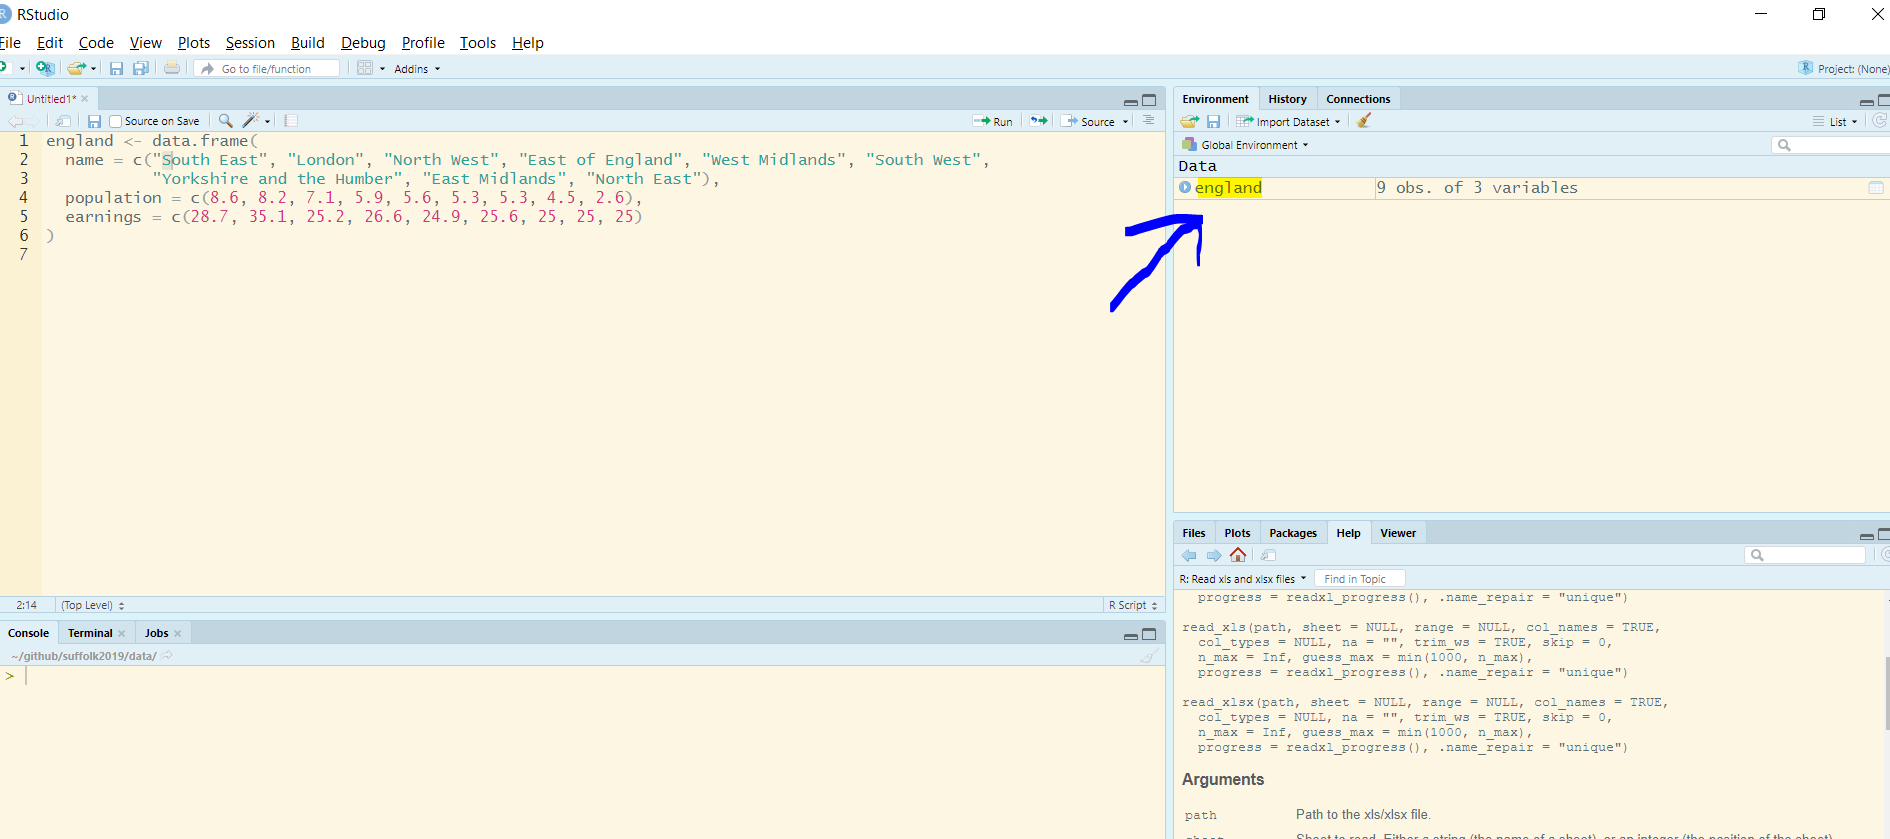
\includegraphics{./img/dataframe_in_spreadsheet_view.png}

Alternatively, you can call the object name to display the dataset in the console window. Let's do so:

\begin{Shaded}
\begin{Highlighting}[]
\NormalTok{england}
\end{Highlighting}
\end{Shaded}

\begin{verbatim}
                      name population earnings
1               South East        8.6     28.7
2                   London        8.2     35.1
3               North West        7.1     25.2
4          East of England        5.9     26.6
5            West Midlands        5.6     24.9
6               South West        5.3     25.6
7 Yorkshire and the Humber        5.3     25.0
8            East Midlands        4.5     25.0
9               North East        2.6     25.0
\end{verbatim}

Often, datasets are too long to be viewed to in the console window. It is a good idea to look at the first couple of rows of a datasets to get an overview of its contents. We use the square brackets \texttt{{[}{]}} to view the first five rows and all columns.

\begin{Shaded}
\begin{Highlighting}[]
\NormalTok{england[}\DecValTok{1}\OperatorTok{:}\DecValTok{5}\NormalTok{, ]}
\end{Highlighting}
\end{Shaded}

\begin{verbatim}
             name population earnings
1      South East        8.6     28.7
2          London        8.2     35.1
3      North West        7.1     25.2
4 East of England        5.9     26.6
5   West Midlands        5.6     24.9
\end{verbatim}

v
Columns in a dataframe have names. We will often need to know the name of a column/variable to access it. We use the \texttt{names()} function to view all variable names in a dataframe.

\begin{Shaded}
\begin{Highlighting}[]
\KeywordTok{names}\NormalTok{(england)}
\end{Highlighting}
\end{Shaded}

\begin{verbatim}
[1] "name"       "population" "earnings"  
\end{verbatim}

We can access the earnings variable in multiple ways. First, we can use the \texttt{\$} operator. We write the name of the dataset object, followed by the \texttt{\$}, followed by the variable name like so:

\begin{Shaded}
\begin{Highlighting}[]
\NormalTok{england}\OperatorTok{$}\NormalTok{earnings}
\end{Highlighting}
\end{Shaded}

\begin{verbatim}
[1] 28.7 35.1 25.2 26.6 24.9 25.6 25.0 25.0 25.0
\end{verbatim}

We can also use the square brackets to access the earnings column.

\begin{Shaded}
\begin{Highlighting}[]
\NormalTok{england[, }\StringTok{"earnings"}\NormalTok{ ]}
\end{Highlighting}
\end{Shaded}

\begin{verbatim}
[1] 28.7 35.1 25.2 26.6 24.9 25.6 25.0 25.0 25.0
\end{verbatim}

The square brackets are sometimes preferred because we could access multiple columns at once like so:

\begin{Shaded}
\begin{Highlighting}[]
\NormalTok{england[, }\KeywordTok{c}\NormalTok{(}\StringTok{"name"}\NormalTok{, }\StringTok{"earnings"}\NormalTok{) ]}
\end{Highlighting}
\end{Shaded}

\begin{verbatim}
                      name earnings
1               South East     28.7
2                   London     35.1
3               North West     25.2
4          East of England     26.6
5            West Midlands     24.9
6               South West     25.6
7 Yorkshire and the Humber     25.0
8            East Midlands     25.0
9               North East     25.0
\end{verbatim}

Variables come in different types such as numbers, text, logical (true/false). We need to know the type of a variable because the type affects statistical analysis. We use the \texttt{str()} function to check the type of each variable in our dataset.

\begin{Shaded}
\begin{Highlighting}[]
\KeywordTok{str}\NormalTok{(england)}
\end{Highlighting}
\end{Shaded}

\begin{verbatim}
'data.frame':   9 obs. of  3 variables:
 $ name      : Factor w/ 9 levels "East Midlands",..: 6 3 5 2 8 7 9 1 4
 $ population: num  8.6 8.2 7.1 5.9 5.6 5.3 5.3 4.5 2.6
 $ earnings  : num  28.7 35.1 25.2 26.6 24.9 25.6 25 25 25
\end{verbatim}

The first variable in our dataset is a factor variable. Factors are categorical variables. Categories are mutually exclusive but they do not imply an ordering. For instance, ``East of England'' is not more or less than ``West Midlands''. The variables population and earnings are both numeric variables.

\begin{Shaded}
\begin{Highlighting}[]
\KeywordTok{str}\NormalTok{(england)}
\end{Highlighting}
\end{Shaded}

\begin{verbatim}
'data.frame':   9 obs. of  3 variables:
 $ name      : Factor w/ 9 levels "East Midlands",..: 6 3 5 2 8 7 9 1 4
 $ population: num  8.6 8.2 7.1 5.9 5.6 5.3 5.3 4.5 2.6
 $ earnings  : num  28.7 35.1 25.2 26.6 24.9 25.6 25 25 25
\end{verbatim}

\hypertarget{amending-data-frames}{%
\subsubsection{Amending data frames}\label{amending-data-frames}}

Amending data sets usually involves adding rows or columns or removing rows or columns. We start by adding a new variable to our dataset which contains the percent of the population on income support.

To create a new variable we simply assign a new vector to the dataframe object like so:

\begin{Shaded}
\begin{Highlighting}[]
\NormalTok{england}\OperatorTok{$}\NormalTok{pct_on_support <-}\StringTok{ }\KeywordTok{c}\NormalTok{(}\DecValTok{3}\NormalTok{, }\FloatTok{5.3}\NormalTok{, }\FloatTok{5.3}\NormalTok{, }\FloatTok{3.5}\NormalTok{, }\FloatTok{5.1}\NormalTok{, }\FloatTok{3.3}\NormalTok{, }\FloatTok{5.2}\NormalTok{, }\FloatTok{4.2}\NormalTok{, }\FloatTok{6.1}\NormalTok{)}
\end{Highlighting}
\end{Shaded}

We call the dataframe object to view our changes.

\begin{Shaded}
\begin{Highlighting}[]
\NormalTok{england}
\end{Highlighting}
\end{Shaded}

\begin{verbatim}
                      name population earnings pct_on_support
1               South East        8.6     28.7            3.0
2                   London        8.2     35.1            5.3
3               North West        7.1     25.2            5.3
4          East of England        5.9     26.6            3.5
5            West Midlands        5.6     24.9            5.1
6               South West        5.3     25.6            3.3
7 Yorkshire and the Humber        5.3     25.0            5.2
8            East Midlands        4.5     25.0            4.2
9               North East        2.6     25.0            6.1
\end{verbatim}

We can delete the variable we just created by assigning \texttt{NULL} to it.

\begin{Shaded}
\begin{Highlighting}[]
\NormalTok{england}\OperatorTok{$}\NormalTok{pct_on_support <-}\StringTok{ }\OtherTok{NULL}
\end{Highlighting}
\end{Shaded}

Let's view our most recent changes.

\begin{Shaded}
\begin{Highlighting}[]
\NormalTok{england}
\end{Highlighting}
\end{Shaded}

\begin{verbatim}
                      name population earnings
1               South East        8.6     28.7
2                   London        8.2     35.1
3               North West        7.1     25.2
4          East of England        5.9     26.6
5            West Midlands        5.6     24.9
6               South West        5.3     25.6
7 Yorkshire and the Humber        5.3     25.0
8            East Midlands        4.5     25.0
9               North East        2.6     25.0
\end{verbatim}

Adding a new row to a dataset means adding an observation. Let's add Brittany to our dataset. We need to fill in a value for each variable. If, we do not know a value, we declare it as missing. Missings are \texttt{NA} for numeric variables and \texttt{""} for character variables. We use the \texttt{rbind()} function (row bind) to add a row to our dataset.

\begin{Shaded}
\begin{Highlighting}[]
\NormalTok{england <-}\StringTok{ }\KeywordTok{rbind}\NormalTok{(england,  }\KeywordTok{c}\NormalTok{(}\StringTok{"Brittany"}\NormalTok{, }\FloatTok{4.5}\NormalTok{, }\OtherTok{NA}\NormalTok{) )}
\end{Highlighting}
\end{Shaded}

\begin{verbatim}
Warning in `[<-.factor`(`*tmp*`, ri, value = "Brittany"): invalid factor
level, NA generated
\end{verbatim}

Let's examine our dataframe.

\begin{Shaded}
\begin{Highlighting}[]
\NormalTok{england}
\end{Highlighting}
\end{Shaded}

\begin{verbatim}
                       name population earnings
1                South East        8.6     28.7
2                    London        8.2     35.1
3                North West        7.1     25.2
4           East of England        5.9     26.6
5             West Midlands        5.6     24.9
6                South West        5.3     25.6
7  Yorkshire and the Humber        5.3       25
8             East Midlands        4.5       25
9                North East        2.6       25
10                     <NA>        4.5     <NA>
\end{verbatim}

We were not allowed to enter ``Brittany'' as a value for the name variable. This is because the variable is a factor. While it is possible to add new levels to a factor (categories such as ``Midlands'' are called levels), it involves a bit more advanced programming. We will solve this problem later in the type coercion section.

\hypertarget{saving-data-frames}{%
\subsubsection{Saving data frames}\label{saving-data-frames}}

Datasets can be exported in many different file formats. We recommend exporting files as ``.csv'' files because csv is a very common file type. Such files can be handled by all statistical packages including Microsoft's Excel. We need to provide five arguments.

\begin{longtable}[]{@{}ll@{}}
\toprule
Argument & Description\tabularnewline
\midrule
\endhead
x & The name of the object\tabularnewline
file & The file name\tabularnewline
sep & The symbol that separates columns\tabularnewline
col.names & = TRUE saves the variable names (recommended)\tabularnewline
row.names & = FALSE omits the row names (recommended)\tabularnewline
\bottomrule
\end{longtable}

\begin{Shaded}
\begin{Highlighting}[]
\KeywordTok{write.table}\NormalTok{(}\DataTypeTok{x =}\NormalTok{ england, }\DataTypeTok{file =} \StringTok{"england.csv"}\NormalTok{, }\DataTypeTok{sep =} \StringTok{","}\NormalTok{, }\DataTypeTok{col.names =} \OtherTok{TRUE}\NormalTok{, }\DataTypeTok{row.names =} \OtherTok{FALSE}\NormalTok{)}
\end{Highlighting}
\end{Shaded}

\hypertarget{type-coercion}{%
\section{Type coercion}\label{type-coercion}}

\hypertarget{seminar-3}{%
\subsection{Seminar}\label{seminar-3}}

We often need to change the type of a variable. This can be necessary to clean data or because we add a new level to a factor like in the previous section on amending data frames. We begin by loading the england dataset that we created previously.

\begin{Shaded}
\begin{Highlighting}[]
\NormalTok{england <-}\StringTok{ }\KeywordTok{read.csv}\NormalTok{(}\DataTypeTok{file =} \StringTok{"england.csv"}\NormalTok{, }\DataTypeTok{sep =} \StringTok{","}\NormalTok{, }\DataTypeTok{header =} \OtherTok{TRUE}\NormalTok{)}
\end{Highlighting}
\end{Shaded}

Recall that we could not add ``Brittany'' as a name to our variable. This was because the variable name is stored as a factor and ``Brittany'' was a new category. The easiest way to add the name ``Brittany'' is to convert the name variable into a character variable.

\hypertarget{coerce-a-factor-to-character}{%
\subsubsection{Coerce a factor to character}\label{coerce-a-factor-to-character}}

Let's check our england dataset's variable types.
.

\begin{Shaded}
\begin{Highlighting}[]
\KeywordTok{str}\NormalTok{(england)}
\end{Highlighting}
\end{Shaded}

\begin{verbatim}
'data.frame':   10 obs. of  3 variables:
 $ name      : Factor w/ 9 levels "East Midlands",..: 6 3 5 2 8 7 9 1 4 NA
 $ population: num  8.6 8.2 7.1 5.9 5.6 5.3 5.3 4.5 2.6 4.5
 $ earnings  : num  28.7 35.1 25.2 26.6 24.9 25.6 25 25 25 NA
\end{verbatim}

The variable ``name'' is a factor variable and needs to be converted to a character variable. We coerce the variable into a different type using the \texttt{as.character()} function.

\begin{Shaded}
\begin{Highlighting}[]
\NormalTok{england}\OperatorTok{$}\NormalTok{name <-}\StringTok{ }\KeywordTok{as.character}\NormalTok{(england}\OperatorTok{$}\NormalTok{name)}
\end{Highlighting}
\end{Shaded}

Let's inspect the variable types of our dataset again:

\begin{Shaded}
\begin{Highlighting}[]
\KeywordTok{str}\NormalTok{(england)}
\end{Highlighting}
\end{Shaded}

\begin{verbatim}
'data.frame':   10 obs. of  3 variables:
 $ name      : chr  "South East" "London" "North West" "East of England" ...
 $ population: num  8.6 8.2 7.1 5.9 5.6 5.3 5.3 4.5 2.6 4.5
 $ earnings  : num  28.7 35.1 25.2 26.6 24.9 25.6 25 25 25 NA
\end{verbatim}

The variable name is now a character variable. We now change the last value of the name variable into Brittany.

\begin{Shaded}
\begin{Highlighting}[]
\NormalTok{england}\OperatorTok{$}\NormalTok{name[ }\KeywordTok{length}\NormalTok{(england}\OperatorTok{$}\NormalTok{name) ] <-}\StringTok{ "Brittany"}
\end{Highlighting}
\end{Shaded}

Let's inspect our change.

\begin{Shaded}
\begin{Highlighting}[]
\NormalTok{england}
\end{Highlighting}
\end{Shaded}

\begin{verbatim}
                       name population earnings
1                South East        8.6     28.7
2                    London        8.2     35.1
3                North West        7.1     25.2
4           East of England        5.9     26.6
5             West Midlands        5.6     24.9
6                South West        5.3     25.6
7  Yorkshire and the Humber        5.3     25.0
8             East Midlands        4.5     25.0
9                North East        2.6     25.0
10                 Brittany        4.5       NA
\end{verbatim}

\hypertarget{coerce-a-character-variable-into-a-factor-variable}{%
\subsubsection{Coerce a character variable into a factor variable}\label{coerce-a-character-variable-into-a-factor-variable}}

We can now easily convert the variable type back from character into a factor with the \texttt{as.factor()} function like so:

\begin{Shaded}
\begin{Highlighting}[]
\NormalTok{england}\OperatorTok{$}\NormalTok{name <-}\StringTok{ }\KeywordTok{as.factor}\NormalTok{(england}\OperatorTok{$}\NormalTok{name)}
\KeywordTok{str}\NormalTok{(england)}
\end{Highlighting}
\end{Shaded}

\begin{verbatim}
'data.frame':   10 obs. of  3 variables:
 $ name      : Factor w/ 10 levels "Brittany","East Midlands",..: 7 4 6 3 9 8 10 2 5 1
 $ population: num  8.6 8.2 7.1 5.9 5.6 5.3 5.3 4.5 2.6 4.5
 $ earnings  : num  28.7 35.1 25.2 26.6 24.9 25.6 25 25 25 NA
\end{verbatim}

\hypertarget{coerce-a-character-variable-into-a-numeric-variable}{%
\subsubsection{Coerce a character variable into a numeric variable}\label{coerce-a-character-variable-into-a-numeric-variable}}

In R missing vlues are called \texttt{NA} for numeric types and \texttt{""} for character types. When we use load third party data, the coding often differs. This can happen, for instance, due to data entry errors.

We simulate a data entry error by changing the population value of Brittany to a character value.

\begin{Shaded}
\begin{Highlighting}[]
\NormalTok{england}\OperatorTok{$}\NormalTok{population[ }\KeywordTok{length}\NormalTok{(england}\OperatorTok{$}\NormalTok{population) ] <-}\StringTok{ "mistake"}
\KeywordTok{str}\NormalTok{(england)}
\end{Highlighting}
\end{Shaded}

\begin{verbatim}
'data.frame':   10 obs. of  3 variables:
 $ name      : Factor w/ 10 levels "Brittany","East Midlands",..: 7 4 6 3 9 8 10 2 5 1
 $ population: chr  "8.6" "8.2" "7.1" "5.9" ...
 $ earnings  : num  28.7 35.1 25.2 26.6 24.9 25.6 25 25 25 NA
\end{verbatim}

Notice, that the variable population is now a character vector instead of a numeric vector. Whenever numbers and text are mixed, R will automatically treat the vector as a character vector.

We can convert the population variable back into a numeric variable using the \texttt{as.numeric()} function. All values that are not recognised as numbers will be changed to \texttt{NA}.

\begin{Shaded}
\begin{Highlighting}[]
\NormalTok{england}\OperatorTok{$}\NormalTok{population <-}\StringTok{ }\KeywordTok{as.numeric}\NormalTok{(england}\OperatorTok{$}\NormalTok{population)}
\end{Highlighting}
\end{Shaded}

\begin{verbatim}
Warning: NAs introduced by coercion
\end{verbatim}

\begin{Shaded}
\begin{Highlighting}[]
\KeywordTok{str}\NormalTok{(england)}
\end{Highlighting}
\end{Shaded}

\begin{verbatim}
'data.frame':   10 obs. of  3 variables:
 $ name      : Factor w/ 10 levels "Brittany","East Midlands",..: 7 4 6 3 9 8 10 2 5 1
 $ population: num  8.6 8.2 7.1 5.9 5.6 5.3 5.3 4.5 2.6 NA
 $ earnings  : num  28.7 35.1 25.2 26.6 24.9 25.6 25 25 25 NA
\end{verbatim}

\begin{Shaded}
\begin{Highlighting}[]
\NormalTok{england}
\end{Highlighting}
\end{Shaded}

\begin{verbatim}
                       name population earnings
1                South East        8.6     28.7
2                    London        8.2     35.1
3                North West        7.1     25.2
4           East of England        5.9     26.6
5             West Midlands        5.6     24.9
6                South West        5.3     25.6
7  Yorkshire and the Humber        5.3     25.0
8             East Midlands        4.5     25.0
9                North East        2.6     25.0
10                 Brittany         NA       NA
\end{verbatim}

\hypertarget{loops-and-conditions}{%
\section{Loops and conditions}\label{loops-and-conditions}}

\hypertarget{seminar-4}{%
\subsection{Seminar}\label{seminar-4}}

In this section, we introduce loops and conditional statements. Loops are generally useful, when we want to carry out the same operation over and over. Conditions are logical statements that are evaluated and if the statement is true a different operation is carried out than if the statement is false. We may, for instance, be interested in the average crime rate in our sample but only if the respondents are female. To do so, we need conditional statements.

\hypertarget{for-loops}{%
\subsubsection{For loops}\label{for-loops}}

Loops are useful when we need to carry out similar operations repeatedly. A for loop is an easy way to do this. We will create a simple ``for loop'' like so:

\begin{Shaded}
\begin{Highlighting}[]
\ControlFlowTok{for}\NormalTok{ (idx }\ControlFlowTok{in} \DecValTok{1}\OperatorTok{:}\DecValTok{7}\NormalTok{)\{}
  \KeywordTok{print}\NormalTok{( idx )}
\NormalTok{\}}
\end{Highlighting}
\end{Shaded}

\begin{verbatim}
[1] 1
[1] 2
[1] 3
[1] 4
[1] 5
[1] 6
[1] 7
\end{verbatim}

In the above code, the \texttt{for()} function initiates the loop. We loop from 1 through 7 and \texttt{idx} takes the values from 1 to 7 iteratively. We can write code within the curly braces. Here, we simply print the current loop iteration.

We can create nested loops, i.e.~loops within loops like so:

\begin{Shaded}
\begin{Highlighting}[]
\CommentTok{# first loop}
\ControlFlowTok{for}\NormalTok{ (idx }\ControlFlowTok{in} \DecValTok{1}\OperatorTok{:}\DecValTok{7}\NormalTok{)\{}
  
  \CommentTok{# second loop}
  \ControlFlowTok{for}\NormalTok{ (idx2 }\ControlFlowTok{in} \DecValTok{1}\OperatorTok{:}\StringTok{ }\DecValTok{7}\NormalTok{)\{}
    
    \ControlFlowTok{if}\NormalTok{ (idx }\OperatorTok{<}\StringTok{ }\NormalTok{idx2) }\KeywordTok{print}\NormalTok{(}\StringTok{"idx1 is smaller than idx2"}\NormalTok{)}
    \ControlFlowTok{else} \KeywordTok{print}\NormalTok{(}\StringTok{"idx1 is larger than idx2"}\NormalTok{)}
    
\NormalTok{  \} }\CommentTok{# end of second loop}
\NormalTok{\} }\CommentTok{# end of first loop}
\end{Highlighting}
\end{Shaded}

\begin{verbatim}
[1] "idx1 is larger than idx2"
[1] "idx1 is smaller than idx2"
[1] "idx1 is smaller than idx2"
[1] "idx1 is smaller than idx2"
[1] "idx1 is smaller than idx2"
[1] "idx1 is smaller than idx2"
[1] "idx1 is smaller than idx2"
[1] "idx1 is larger than idx2"
[1] "idx1 is larger than idx2"
[1] "idx1 is smaller than idx2"
[1] "idx1 is smaller than idx2"
[1] "idx1 is smaller than idx2"
[1] "idx1 is smaller than idx2"
[1] "idx1 is smaller than idx2"
[1] "idx1 is larger than idx2"
[1] "idx1 is larger than idx2"
[1] "idx1 is larger than idx2"
[1] "idx1 is smaller than idx2"
[1] "idx1 is smaller than idx2"
[1] "idx1 is smaller than idx2"
[1] "idx1 is smaller than idx2"
[1] "idx1 is larger than idx2"
[1] "idx1 is larger than idx2"
[1] "idx1 is larger than idx2"
[1] "idx1 is larger than idx2"
[1] "idx1 is smaller than idx2"
[1] "idx1 is smaller than idx2"
[1] "idx1 is smaller than idx2"
[1] "idx1 is larger than idx2"
[1] "idx1 is larger than idx2"
[1] "idx1 is larger than idx2"
[1] "idx1 is larger than idx2"
[1] "idx1 is larger than idx2"
[1] "idx1 is smaller than idx2"
[1] "idx1 is smaller than idx2"
[1] "idx1 is larger than idx2"
[1] "idx1 is larger than idx2"
[1] "idx1 is larger than idx2"
[1] "idx1 is larger than idx2"
[1] "idx1 is larger than idx2"
[1] "idx1 is larger than idx2"
[1] "idx1 is smaller than idx2"
[1] "idx1 is larger than idx2"
[1] "idx1 is larger than idx2"
[1] "idx1 is larger than idx2"
[1] "idx1 is larger than idx2"
[1] "idx1 is larger than idx2"
[1] "idx1 is larger than idx2"
[1] "idx1 is larger than idx2"
\end{verbatim}

While this is a toy example, it illustrates how we could do pairwise comparisons between observations in our dataset. We also added an if/else condition using the functions \texttt{if()} and \texttt{else}. If the if statement is TRUE the first statement is printed and if not the second statement is printed.

\hypertarget{conditions}{%
\subsubsection{Conditions}\label{conditions}}

To illustrate the use of conditions we load the non-western foreigners dataset.

\begin{Shaded}
\begin{Highlighting}[]
\NormalTok{dat1 <-}\StringTok{ }\KeywordTok{read.csv}\NormalTok{(}\StringTok{"non_western_immigrants.csv"}\NormalTok{)}
\end{Highlighting}
\end{Shaded}

\begin{longtable}[]{@{}ll@{}}
\toprule
\begin{minipage}[b]{0.11\columnwidth}\raggedright
Variable Name\strut
\end{minipage} & \begin{minipage}[b]{0.83\columnwidth}\raggedright
Description\strut
\end{minipage}\tabularnewline
\midrule
\endhead
\begin{minipage}[t]{0.11\columnwidth}\raggedright
IMMBRIT\strut
\end{minipage} & \begin{minipage}[t]{0.83\columnwidth}\raggedright
Out of every 100 people in Britain, how many do you think are immigrants from Non-western countries?\strut
\end{minipage}\tabularnewline
\begin{minipage}[t]{0.11\columnwidth}\raggedright
over.estimate\strut
\end{minipage} & \begin{minipage}[t]{0.83\columnwidth}\raggedright
1 if estimate is higher than 10.7\%.\strut
\end{minipage}\tabularnewline
\begin{minipage}[t]{0.11\columnwidth}\raggedright
RSex\strut
\end{minipage} & \begin{minipage}[t]{0.83\columnwidth}\raggedright
1 = male, 2 = female\strut
\end{minipage}\tabularnewline
\begin{minipage}[t]{0.11\columnwidth}\raggedright
RAge\strut
\end{minipage} & \begin{minipage}[t]{0.83\columnwidth}\raggedright
Age of respondent\strut
\end{minipage}\tabularnewline
\begin{minipage}[t]{0.11\columnwidth}\raggedright
Househld\strut
\end{minipage} & \begin{minipage}[t]{0.83\columnwidth}\raggedright
Number of people living in respondent's household\strut
\end{minipage}\tabularnewline
\begin{minipage}[t]{0.11\columnwidth}\raggedright
Cons, Lab, SNP, Ukip, BNP, GP, party.other\strut
\end{minipage} & \begin{minipage}[t]{0.83\columnwidth}\raggedright
Party self-identification\strut
\end{minipage}\tabularnewline
\begin{minipage}[t]{0.11\columnwidth}\raggedright
paper\strut
\end{minipage} & \begin{minipage}[t]{0.83\columnwidth}\raggedright
Do you normally read any daily morning newspaper 3+ times/week?\strut
\end{minipage}\tabularnewline
\begin{minipage}[t]{0.11\columnwidth}\raggedright
WWWhourspW\strut
\end{minipage} & \begin{minipage}[t]{0.83\columnwidth}\raggedright
How many hours WWW per week?\strut
\end{minipage}\tabularnewline
\begin{minipage}[t]{0.11\columnwidth}\raggedright
religious\strut
\end{minipage} & \begin{minipage}[t]{0.83\columnwidth}\raggedright
Do you regard yourself as belonging to any particular religion?\strut
\end{minipage}\tabularnewline
\begin{minipage}[t]{0.11\columnwidth}\raggedright
employMonths\strut
\end{minipage} & \begin{minipage}[t]{0.83\columnwidth}\raggedright
How many mnths w. present employer?\strut
\end{minipage}\tabularnewline
\begin{minipage}[t]{0.11\columnwidth}\raggedright
urban\strut
\end{minipage} & \begin{minipage}[t]{0.83\columnwidth}\raggedright
Population density, 4 categories (highest density is 4, lowest is 1)\strut
\end{minipage}\tabularnewline
\begin{minipage}[t]{0.11\columnwidth}\raggedright
health.good\strut
\end{minipage} & \begin{minipage}[t]{0.83\columnwidth}\raggedright
How is your health in general for someone of your age? (0: bad, 1: fair, 2: fairly good, 3: good)\strut
\end{minipage}\tabularnewline
\begin{minipage}[t]{0.11\columnwidth}\raggedright
HHInc\strut
\end{minipage} & \begin{minipage}[t]{0.83\columnwidth}\raggedright
Income bands for household, high number = high HH income\strut
\end{minipage}\tabularnewline
\bottomrule
\end{longtable}

The variable \texttt{over.estimate} is equal to 1 if respondents over estimate the number of non-western immigrants in Britain. We will evaluate whether women are more or less likely to over estimate. First, we use the \texttt{mean()} function to assess the overall average value.

\begin{Shaded}
\begin{Highlighting}[]
\KeywordTok{mean}\NormalTok{(dat1}\OperatorTok{$}\NormalTok{over.estimate)}
\end{Highlighting}
\end{Shaded}

\begin{verbatim}
[1] 0.7235462
\end{verbatim}

A mean of 0.72 indicates that 72\% of the 1049 respondents in the dataset over estimate the number of non-western immigrants. To assess whether the number is larger among men than women, we need conditional statements.

We first take the mean of ``over.estimate'' for men:

\begin{Shaded}
\begin{Highlighting}[]
\KeywordTok{mean}\NormalTok{( dat1}\OperatorTok{$}\NormalTok{over.estimate[ dat1}\OperatorTok{$}\NormalTok{RSex}\OperatorTok{==}\DecValTok{1}\NormalTok{ ] )}
\end{Highlighting}
\end{Shaded}

\begin{verbatim}
[1] 0.6527197
\end{verbatim}

Here, we used square brackets to subset the data. The subset that we evaluate is described by the logical statement \texttt{dat1\$RSex==1}. The \texttt{==} operator is a logical equal that is true if a condition is fulfilled and false otherwise. In this case, it is true if the variable ``RSex'' is 1 which stands for men.

Take the mean of over.estimate for women on your own.

\begin{Shaded}
\begin{Highlighting}[]
\KeywordTok{mean}\NormalTok{( dat1}\OperatorTok{$}\NormalTok{over.estimate[ dat1}\OperatorTok{$}\NormalTok{RSex}\OperatorTok{==}\StringTok{ }\DecValTok{2}\NormalTok{] )}
\end{Highlighting}
\end{Shaded}

\begin{verbatim}
[1] 0.7828371
\end{verbatim}

It turns out, that females in our sample over estimate the number of non-western immigrants more. Whether the difference in our sample is systematic, i.e.~whether it would hold in the population as well is a matter that we will return to.

Here we have taken two conditional means and compared them. Doing so is the first step towards statistical inference.

\hypertarget{the-ifelse-function}{%
\subsubsection{The ifelse() function}\label{the-ifelse-function}}

Categorical variables such as ``RSex'' are usually coded 0/1 and the variable name usually refers to the category that is 1. ``RSex'' is a bad variable name because it is not clear whehter the values 1 and 2 refer to males or females.

We will create a new variable called ``female'' that is equal to 1 if the respondent is female and 0 otherwise. We do so using the \texttt{ifelse()} function. The function first evaluates a logical condition and subsequently carries out one operation if the statement is true (yes) and another if the statement is false (no).

\begin{Shaded}
\begin{Highlighting}[]
\NormalTok{dat1}\OperatorTok{$}\NormalTok{female <-}\StringTok{ }\KeywordTok{ifelse}\NormalTok{( dat1}\OperatorTok{$}\NormalTok{RSex }\OperatorTok{==}\StringTok{ }\DecValTok{2}\NormalTok{, }\DataTypeTok{yes =} \DecValTok{1}\NormalTok{, }\DataTypeTok{no =} \DecValTok{0}\NormalTok{ )}
\end{Highlighting}
\end{Shaded}

Let's check whetehr we correctly converted the variable using the \texttt{table()} function which produces a frequency table.

\begin{Shaded}
\begin{Highlighting}[]
\KeywordTok{table}\NormalTok{(dat1}\OperatorTok{$}\NormalTok{RSex)}
\end{Highlighting}
\end{Shaded}

\begin{verbatim}

  1   2 
478 571 
\end{verbatim}

\begin{Shaded}
\begin{Highlighting}[]
\KeywordTok{table}\NormalTok{(dat1}\OperatorTok{$}\NormalTok{female)}
\end{Highlighting}
\end{Shaded}

\begin{verbatim}

  0   1 
478 571 
\end{verbatim}

\hypertarget{visualising-data}{%
\section{Visualising data}\label{visualising-data}}

\hypertarget{seminar-5}{%
\subsection{Seminar}\label{seminar-5}}

In this section, we will learn how to visualise data which is an important step towards understanding relationships better.

The non-western foreingers data is about the subjective perception of immigrants from non-western countries. The perception of immigrants from a context that is not similar to the one's own ,is often used as a proxy for racism. Whether this is a fair measure or not is debatable but let's examine the data from a survey carried out in Britain.

Let's check the codebook of our data.

\begin{tabular}{l|l}
\hline
Variable & Description\\
\hline
IMMBRIT & Out of every 100 people in Britain, how many do you think are immigrants from non-western countries?\\
\hline
over.estimate & 1 if estimate is higher than 10.7\%.\\
\hline
RSex & 1 = male, 2 = female\\
\hline
RAge & Age of respondent\\
\hline
Househld & Number of people living in respondent's household\\
\hline
party identification & 1 = Conservatives, 2 = Labour, 3 = SNP, 4 = Greens, 5 = Ukip, 6 = BNP, 7 = other\\
\hline
paper & Do you normally read any daily morning newspaper 3+ times/week?\\
\hline
WWWhourspW & How many hours WWW per week?\\
\hline
religious & Do you regard yourself as belonging to any particular religion?\\
\hline
employMonths & How many mnths w. present employer?\\
\hline
urban & Population density, 4 categories (highest density is 4, lowest is 1)\\
\hline
health.good & How is your health in general for someone of your age? (0: bad, 1: fair, 2: fairly good, 3: good)\\
\hline
HHInc & Income bands for household, high number = high HH income\\
\hline
\end{tabular}

Let's load the dataset.

\begin{Shaded}
\begin{Highlighting}[]
\NormalTok{dat1 <-}\StringTok{ }\KeywordTok{read.csv}\NormalTok{(}\StringTok{"non_western_immigrants.csv"}\NormalTok{, }\DataTypeTok{stringsAsFactors =} \OtherTok{FALSE}\NormalTok{)}
\end{Highlighting}
\end{Shaded}

We can look at the variable names in our data with the \href{http://bit.ly/R_names}{\texttt{names()}} function.

The \href{http://bit.ly/R_dim}{\texttt{dim()}} function can be used to find out the dimensions of the dataset (dimension 1 = rows, dimension 2 = columns).

\begin{Shaded}
\begin{Highlighting}[]
\KeywordTok{dim}\NormalTok{(dat1)}
\end{Highlighting}
\end{Shaded}

\begin{verbatim}
[1] 1049   13
\end{verbatim}

So, the \href{http://bit.ly/R_dim}{\texttt{dim()}} function tells us that we have data from 1049 respondents with 13 variables for each respondent.

Let's take a quick peek at the first 10 observations to see what the dataset looks like. By default the \href{http://bit.ly/R_head}{\texttt{head()}} function returns the first 6 rows, but let's tell it to return the first 10 rows instead.

\begin{Shaded}
\begin{Highlighting}[]
\KeywordTok{head}\NormalTok{(dat1, }\DataTypeTok{n =} \DecValTok{10}\NormalTok{)}
\end{Highlighting}
\end{Shaded}

\begin{verbatim}
   IMMBRIT over.estimate RSex RAge Househld paper WWWhourspW religious
1        1             0    1   50        2     0          1         0
2       50             1    2   18        3     0          4         0
3       50             1    2   60        1     0          1         0
4       15             1    2   77        2     1          2         1
5       20             1    2   67        1     0          1         1
6       30             1    1   30        4     1         14         0
7       60             1    2   56        2     0          5         1
8        7             0    1   49        1     1          8         0
9       30             1    1   40        4     0          3         1
10       2             0    1   61        3     1          0         1
   employMonths urban health.good HHInc party_self
1            72     4           1    13          2
2            72     4           2     3          7
3           456     3           3     9          7
4            72     1           3     8          7
5            72     3           3     9          7
6            72     1           2     9          7
7           180     1           2    13          3
8           156     4           2    14          7
9           264     2           2    11          3
10           72     1           3     8          1
\end{verbatim}

Finally, let's look at summary statistics of our dataset.

\begin{Shaded}
\begin{Highlighting}[]
\KeywordTok{summary}\NormalTok{(dat1)}
\end{Highlighting}
\end{Shaded}

\begin{verbatim}
    IMMBRIT       over.estimate         RSex            RAge      
 Min.   :  0.00   Min.   :0.0000   Min.   :1.000   Min.   :17.00  
 1st Qu.: 10.00   1st Qu.:0.0000   1st Qu.:1.000   1st Qu.:36.00  
 Median : 25.00   Median :1.0000   Median :2.000   Median :49.00  
 Mean   : 29.03   Mean   :0.7235   Mean   :1.544   Mean   :49.75  
 3rd Qu.: 40.00   3rd Qu.:1.0000   3rd Qu.:2.000   3rd Qu.:62.00  
 Max.   :100.00   Max.   :1.0000   Max.   :2.000   Max.   :99.00  
    Househld         paper          WWWhourspW        religious     
 Min.   :1.000   Min.   :0.0000   Min.   :  0.000   Min.   :0.0000  
 1st Qu.:1.000   1st Qu.:0.0000   1st Qu.:  0.000   1st Qu.:0.0000  
 Median :2.000   Median :0.0000   Median :  2.000   Median :0.0000  
 Mean   :2.392   Mean   :0.4538   Mean   :  5.251   Mean   :0.4929  
 3rd Qu.:3.000   3rd Qu.:1.0000   3rd Qu.:  7.000   3rd Qu.:1.0000  
 Max.   :8.000   Max.   :1.0000   Max.   :100.000   Max.   :1.0000  
  employMonths        urban        health.good        HHInc       
 Min.   :  1.00   Min.   :1.000   Min.   :0.000   Min.   : 1.000  
 1st Qu.: 72.00   1st Qu.:2.000   1st Qu.:2.000   1st Qu.: 6.000  
 Median : 72.00   Median :3.000   Median :2.000   Median : 9.000  
 Mean   : 86.56   Mean   :2.568   Mean   :2.044   Mean   : 9.586  
 3rd Qu.: 72.00   3rd Qu.:3.000   3rd Qu.:3.000   3rd Qu.:13.000  
 Max.   :600.00   Max.   :4.000   Max.   :3.000   Max.   :17.000  
   party_self   
 Min.   :1.000  
 1st Qu.:1.000  
 Median :2.000  
 Mean   :3.825  
 3rd Qu.:7.000  
 Max.   :7.000  
\end{verbatim}

\hypertarget{plots}{%
\subsubsection{Plots}\label{plots}}

We can visualize the data with the help of a boxplot, so let's see how the perception of the number of immigrants is distributed.

\begin{Shaded}
\begin{Highlighting}[]
\CommentTok{# how good are we at guessing immigration}
\KeywordTok{boxplot}\NormalTok{(}
\NormalTok{  dat1}\OperatorTok{$}\NormalTok{IMMBRIT, }
  \DataTypeTok{main =} \StringTok{"Perception of Immigration from Non-Western Countries"}\NormalTok{,}
  \DataTypeTok{ylab =} \StringTok{"Subjective number of immigrants per 100 British"}\NormalTok{, }
  \DataTypeTok{frame.plot =} \OtherTok{FALSE}\NormalTok{, }\DataTypeTok{col =} \StringTok{"darkgray"}
\NormalTok{  )}
\end{Highlighting}
\end{Shaded}

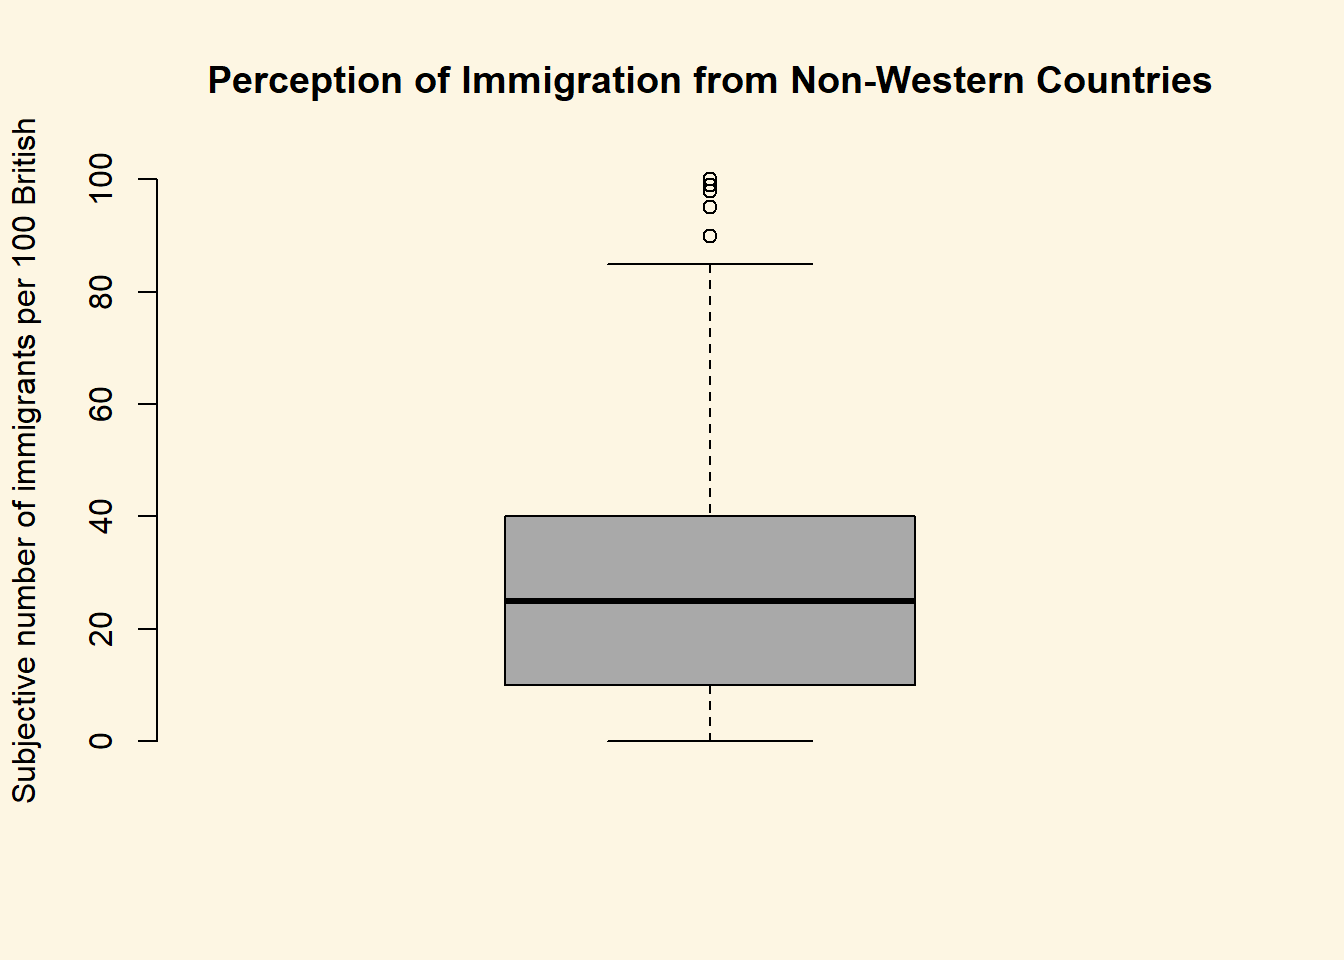
\includegraphics{suffolk2019_files/figure-latex/unnamed-chunk-87-1.pdf}

Notice how the lower whisker is much shorter than the upper one. The distribution is right skewed. The right tail (higher values) is a lot longer. We can see this beter using a density plot. We combine R's \texttt{denisty()} function with the \texttt{plot()} function.

\begin{Shaded}
\begin{Highlighting}[]
\KeywordTok{plot}\NormalTok{(}
  \KeywordTok{density}\NormalTok{(dat1}\OperatorTok{$}\NormalTok{IMMBRIT),}
  \DataTypeTok{bty =} \StringTok{"n"}\NormalTok{,}
  \DataTypeTok{lwd =} \FloatTok{1.5}\NormalTok{,}
  \DataTypeTok{main =} \StringTok{"Perception of Immigration from Non-Western Countries"}\NormalTok{,}
  \DataTypeTok{xlab =} \StringTok{"Subjective number of immigrants per 100 British"}
\NormalTok{  )}
\end{Highlighting}
\end{Shaded}

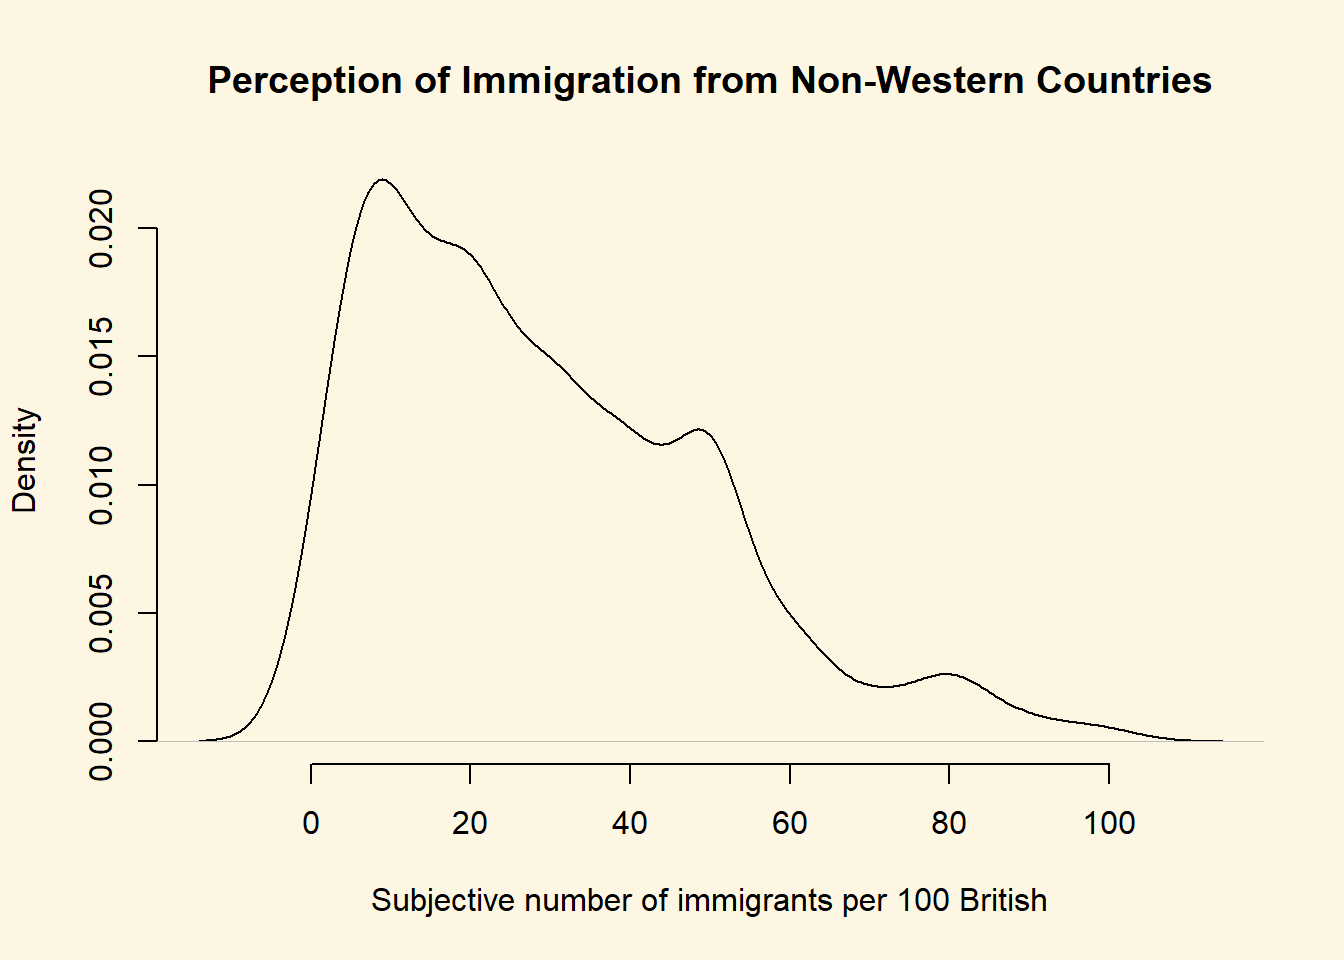
\includegraphics{suffolk2019_files/figure-latex/unnamed-chunk-88-1.pdf}

We can also plot histograms using the \texttt{hist()} function.

\begin{Shaded}
\begin{Highlighting}[]
\CommentTok{# histogram}
\KeywordTok{hist}\NormalTok{( dat1}\OperatorTok{$}\NormalTok{employMonths, }\DataTypeTok{main =} \StringTok{"histogram"}\NormalTok{, }\DataTypeTok{col =} \StringTok{"darkgray"}\NormalTok{)}
\end{Highlighting}
\end{Shaded}

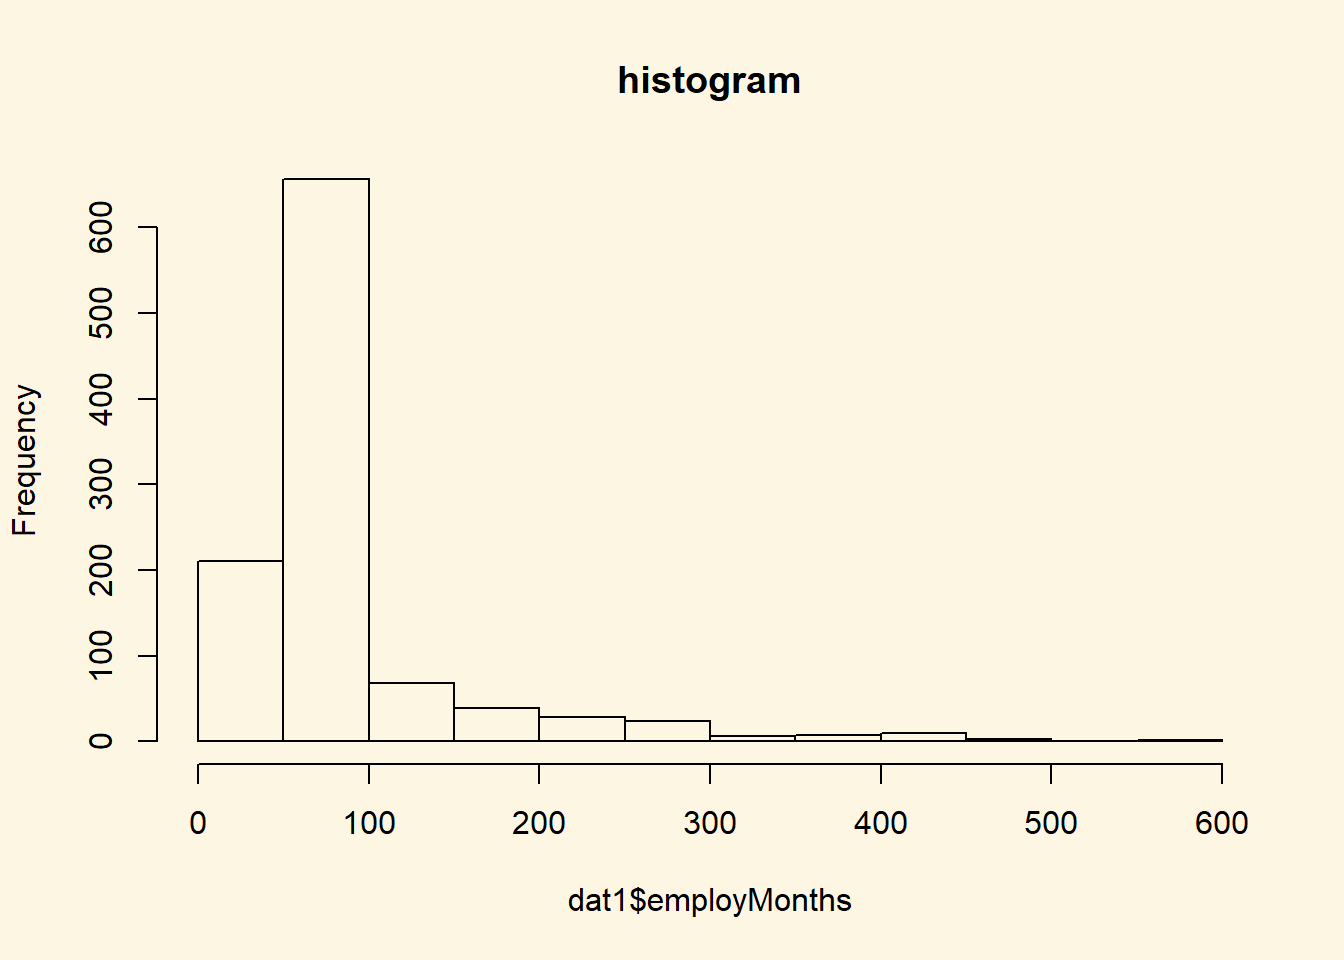
\includegraphics{suffolk2019_files/figure-latex/unnamed-chunk-89-1.pdf}

It is plausible that perception of immigration from Non-Western countries is related to party affiliation. In our dataset, we have a some party affiliation dummies (binary variables). We can use square brackets to subset our data such that we produce a boxplot only for members of the Conservative Party. We first create the binary variables \emph{Cons} and \emph{Lab} for (Conservatives and Labour respectively) using the \texttt{ifelse()} function.

\begin{Shaded}
\begin{Highlighting}[]
\NormalTok{dat1}\OperatorTok{$}\NormalTok{Cons <-}\StringTok{ }\KeywordTok{ifelse}\NormalTok{(dat1}\OperatorTok{$}\NormalTok{party_self }\OperatorTok{==}\StringTok{ }\DecValTok{1}\NormalTok{, }\DataTypeTok{yes =} \DecValTok{1}\NormalTok{, }\DataTypeTok{no =} \DecValTok{0}\NormalTok{)}
\NormalTok{dat1}\OperatorTok{$}\NormalTok{Lab <-}\StringTok{ }\KeywordTok{ifelse}\NormalTok{(dat1}\OperatorTok{$}\NormalTok{party_self }\OperatorTok{==}\StringTok{ }\DecValTok{2}\NormalTok{, }\DataTypeTok{yes =} \DecValTok{1}\NormalTok{, }\DataTypeTok{no =} \DecValTok{0}\NormalTok{)}
\end{Highlighting}
\end{Shaded}

We have a look at the variable \emph{Cons} using the \texttt{table()} function first.

\begin{Shaded}
\begin{Highlighting}[]
\KeywordTok{table}\NormalTok{(dat1}\OperatorTok{$}\NormalTok{Cons)}
\end{Highlighting}
\end{Shaded}

\begin{verbatim}

  0   1 
765 284 
\end{verbatim}

In our data, 284 respondents associate with the Conservative party and 765 do not. We create a boxplot of \emph{IMMBRIT} but only for members of the Conservative Party. We do so by using the square brackets to subset our data.

\begin{Shaded}
\begin{Highlighting}[]
\CommentTok{# boxplot of immbrit for those observations where Cons is 1}
\KeywordTok{boxplot}\NormalTok{(}
\NormalTok{  dat1}\OperatorTok{$}\NormalTok{IMMBRIT[dat1}\OperatorTok{$}\NormalTok{Cons}\OperatorTok{==}\DecValTok{1}\NormalTok{],}
  \DataTypeTok{frame.plot =} \OtherTok{FALSE}\NormalTok{,}
  \DataTypeTok{xlab =} \StringTok{"Conservatives"}\NormalTok{,}
  \DataTypeTok{col =} \StringTok{"blue"}
\NormalTok{  )}
\end{Highlighting}
\end{Shaded}

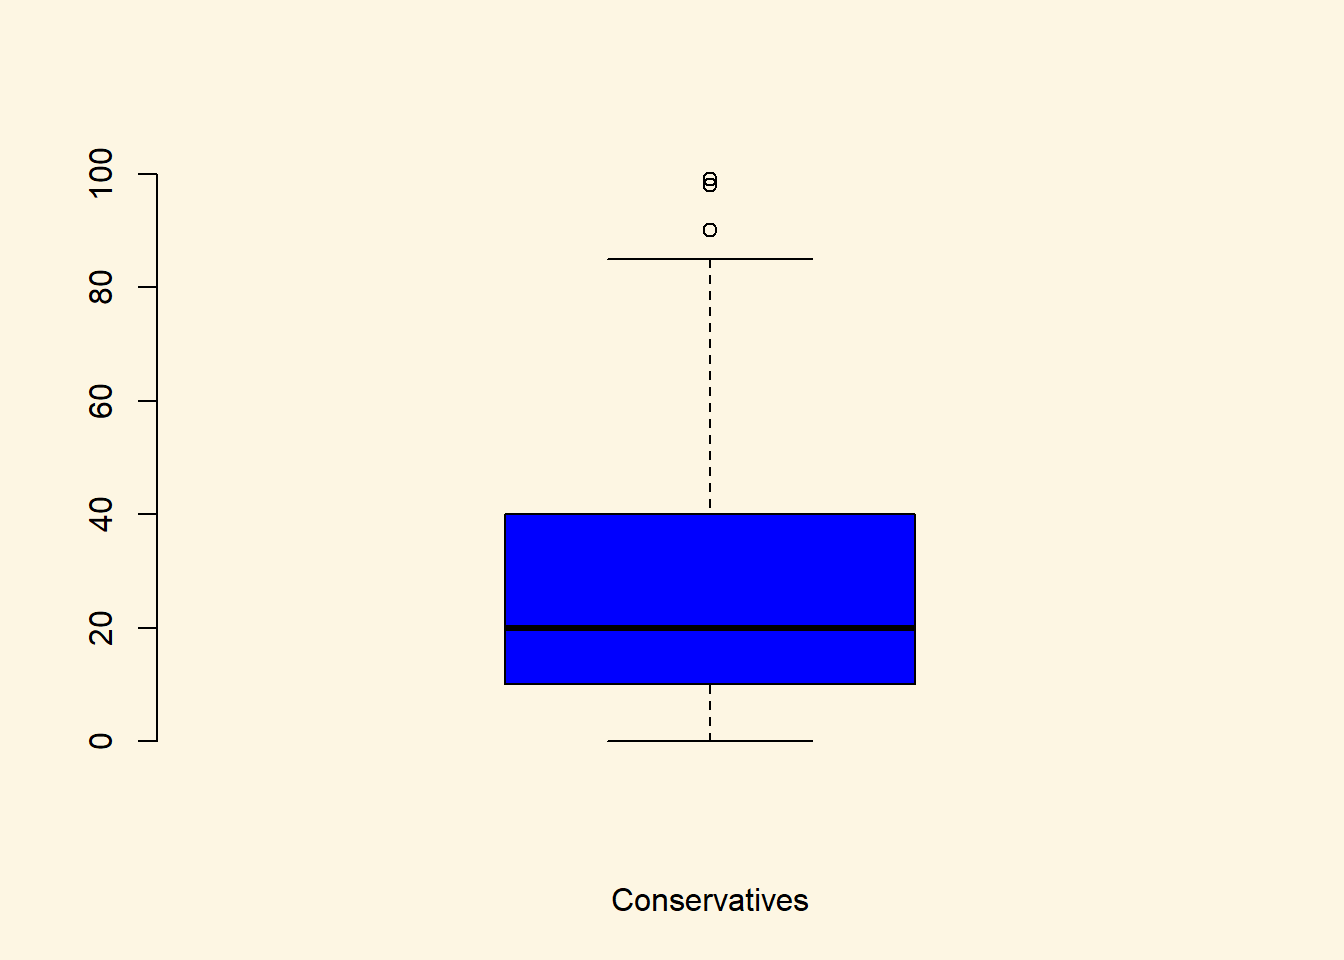
\includegraphics{suffolk2019_files/figure-latex/unnamed-chunk-92-1.pdf}

We would now like to compare the distribution of the perception fo Conservatives to the distribution among Labour respondents. We can subset the data just like we did for the Conservative Party. In addtion, we want to plot the two plots next to each other, i.e., they should be in the same plot. We can achieve this with the \texttt{par()} function and the \texttt{mfrow} argument. This will spilt the plot window into rows and columns. We want 2 columns to plot 2 boxplots next to each other.

\begin{Shaded}
\begin{Highlighting}[]
\CommentTok{# split plot window into 1 row and 2 columns}
\KeywordTok{par}\NormalTok{(}\DataTypeTok{mfrow =} \KeywordTok{c}\NormalTok{(}\DecValTok{1}\NormalTok{,}\DecValTok{2}\NormalTok{))}

\CommentTok{# plot 1}
\KeywordTok{boxplot}\NormalTok{(}
\NormalTok{  dat1}\OperatorTok{$}\NormalTok{IMMBRIT[dat1}\OperatorTok{$}\NormalTok{Cons}\OperatorTok{==}\DecValTok{1}\NormalTok{],}
  \DataTypeTok{frame.plot =} \OtherTok{FALSE}\NormalTok{,}
  \DataTypeTok{xlab =} \StringTok{"Conservatives"}\NormalTok{,}
  \DataTypeTok{col =} \StringTok{"blue"}
\NormalTok{  )}

\CommentTok{# plot 2}
\KeywordTok{boxplot}\NormalTok{(}
\NormalTok{  dat1}\OperatorTok{$}\NormalTok{IMMBRIT[dat1}\OperatorTok{$}\NormalTok{Lab}\OperatorTok{==}\DecValTok{1}\NormalTok{],}
  \DataTypeTok{frame.plot =} \OtherTok{FALSE}\NormalTok{,}
  \DataTypeTok{xlab =} \StringTok{"Labour"}\NormalTok{,}
  \DataTypeTok{col =} \StringTok{"red"}
\NormalTok{  )}
\end{Highlighting}
\end{Shaded}

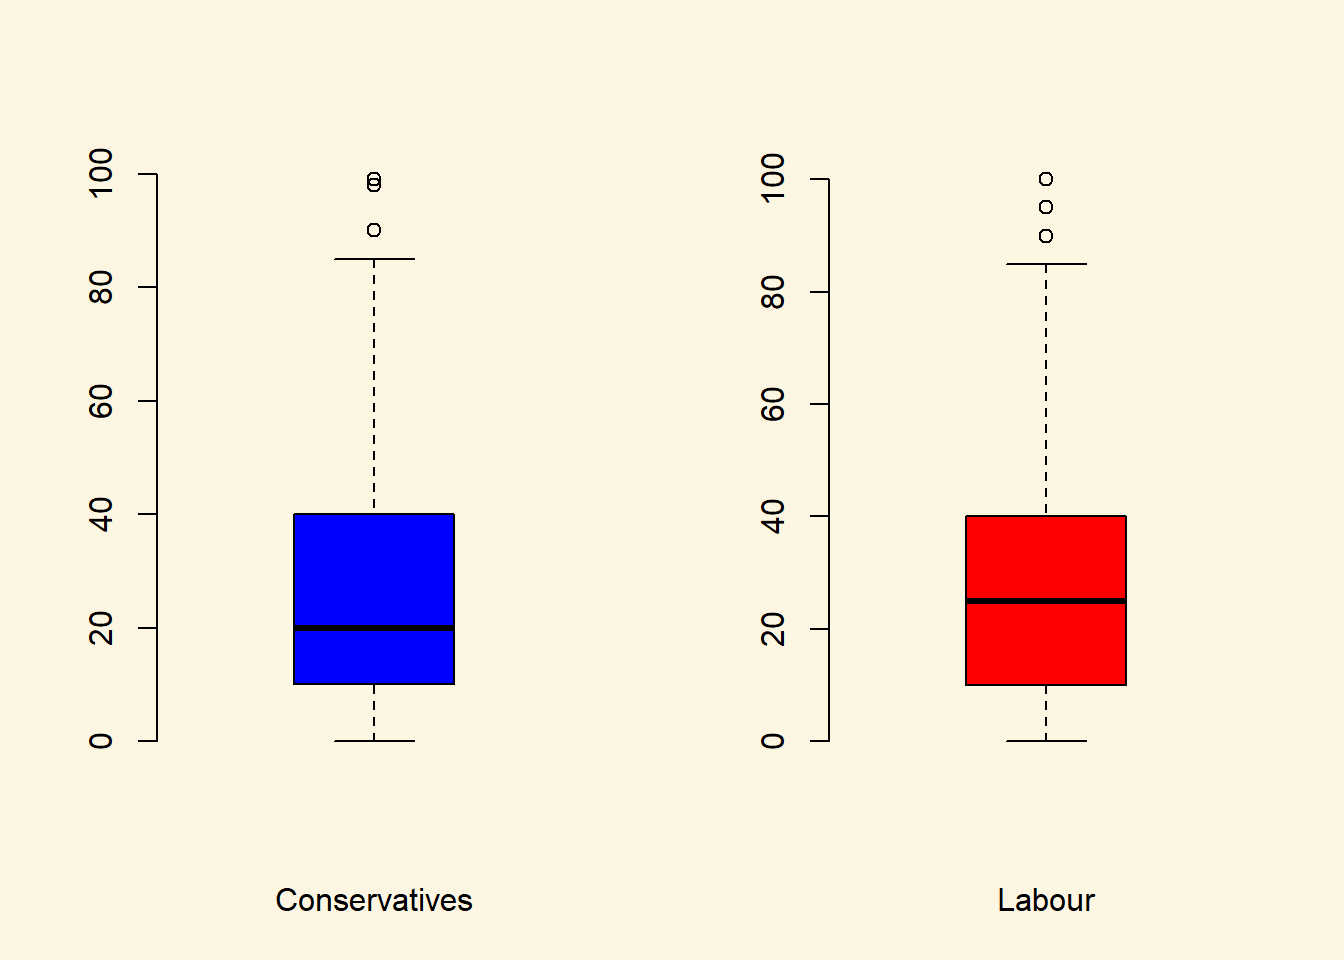
\includegraphics{suffolk2019_files/figure-latex/unnamed-chunk-93-1.pdf}

It is very hard to spot differences. The distributions are similar. The median for Labour respondents is larger which mean that the central Labour respondent over-estimates immigration more than the central Conservative respondent.

You can play around with the non-western foreigners data on your own time. We now turn to a dataset that is integrated in R already. It is called \texttt{longley}. Use the \texttt{help()} function to see what this dataset is about.

\begin{Shaded}
\begin{Highlighting}[]
\KeywordTok{help}\NormalTok{(longley)}
\end{Highlighting}
\end{Shaded}

Let's create a scatterplot with the \texttt{Year} variable on the x-axis and \texttt{Employed} on the y-axis.

\begin{Shaded}
\begin{Highlighting}[]
\KeywordTok{plot}\NormalTok{(}\DataTypeTok{x =}\NormalTok{ longley}\OperatorTok{$}\NormalTok{Year, }\CommentTok{# x-axis variable}
     \DataTypeTok{y =}\NormalTok{ longley}\OperatorTok{$}\NormalTok{Employed, }\CommentTok{# y-axis variable}
     \DataTypeTok{bty =} \StringTok{"n"} \CommentTok{# no box around the plot}
\NormalTok{     )}
\end{Highlighting}
\end{Shaded}

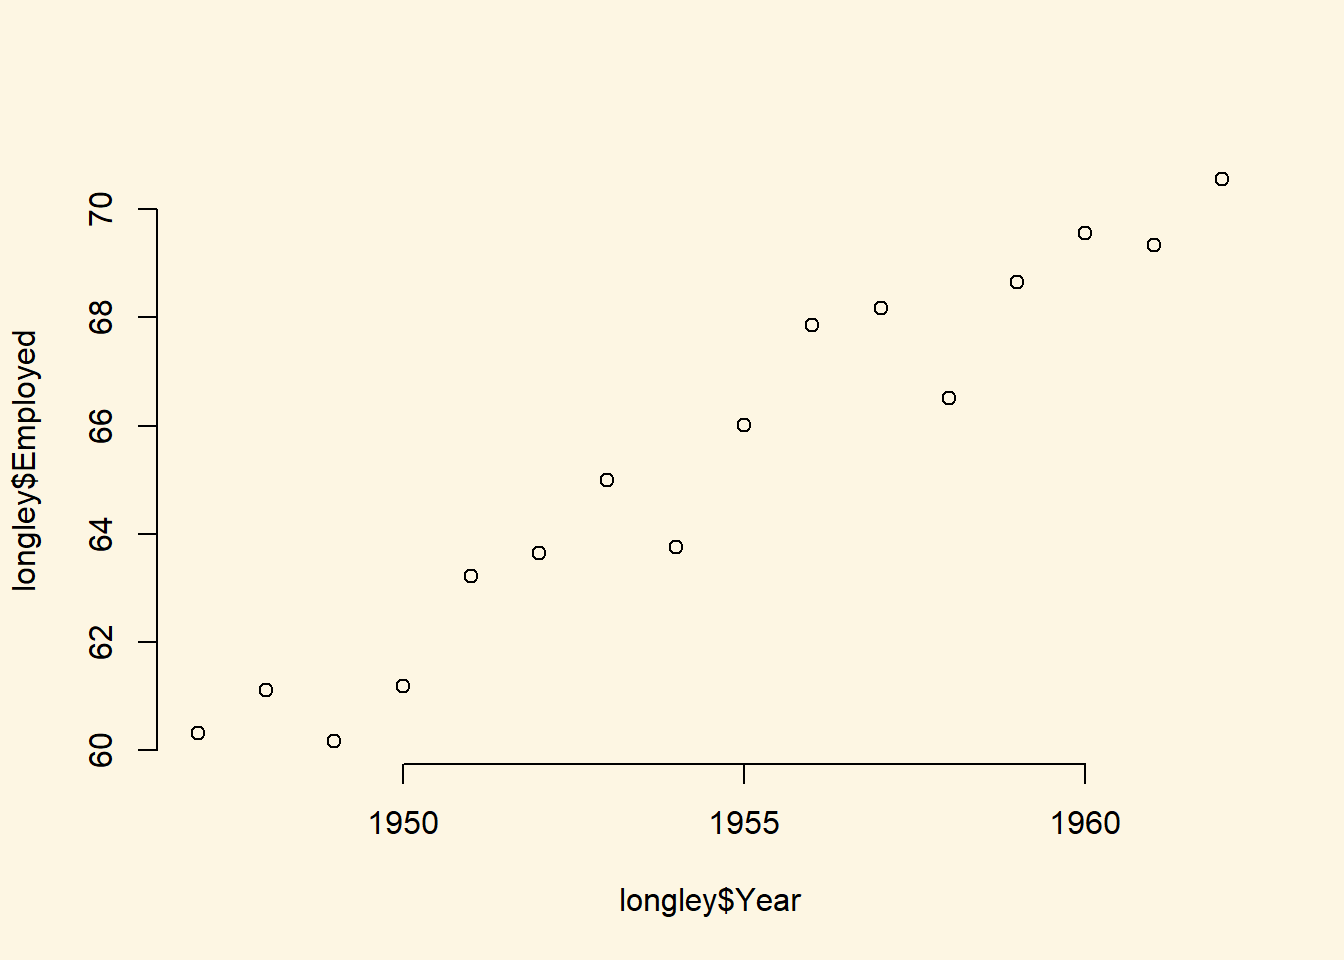
\includegraphics{suffolk2019_files/figure-latex/unnamed-chunk-96-1.pdf}

To create a line plot instead, we use the same function with one additional argument \texttt{type\ =\ "l"}.

\begin{Shaded}
\begin{Highlighting}[]
\KeywordTok{plot}\NormalTok{(longley}\OperatorTok{$}\NormalTok{Year, longley}\OperatorTok{$}\NormalTok{Employed, }\DataTypeTok{type =} \StringTok{"l"}\NormalTok{)}
\end{Highlighting}
\end{Shaded}

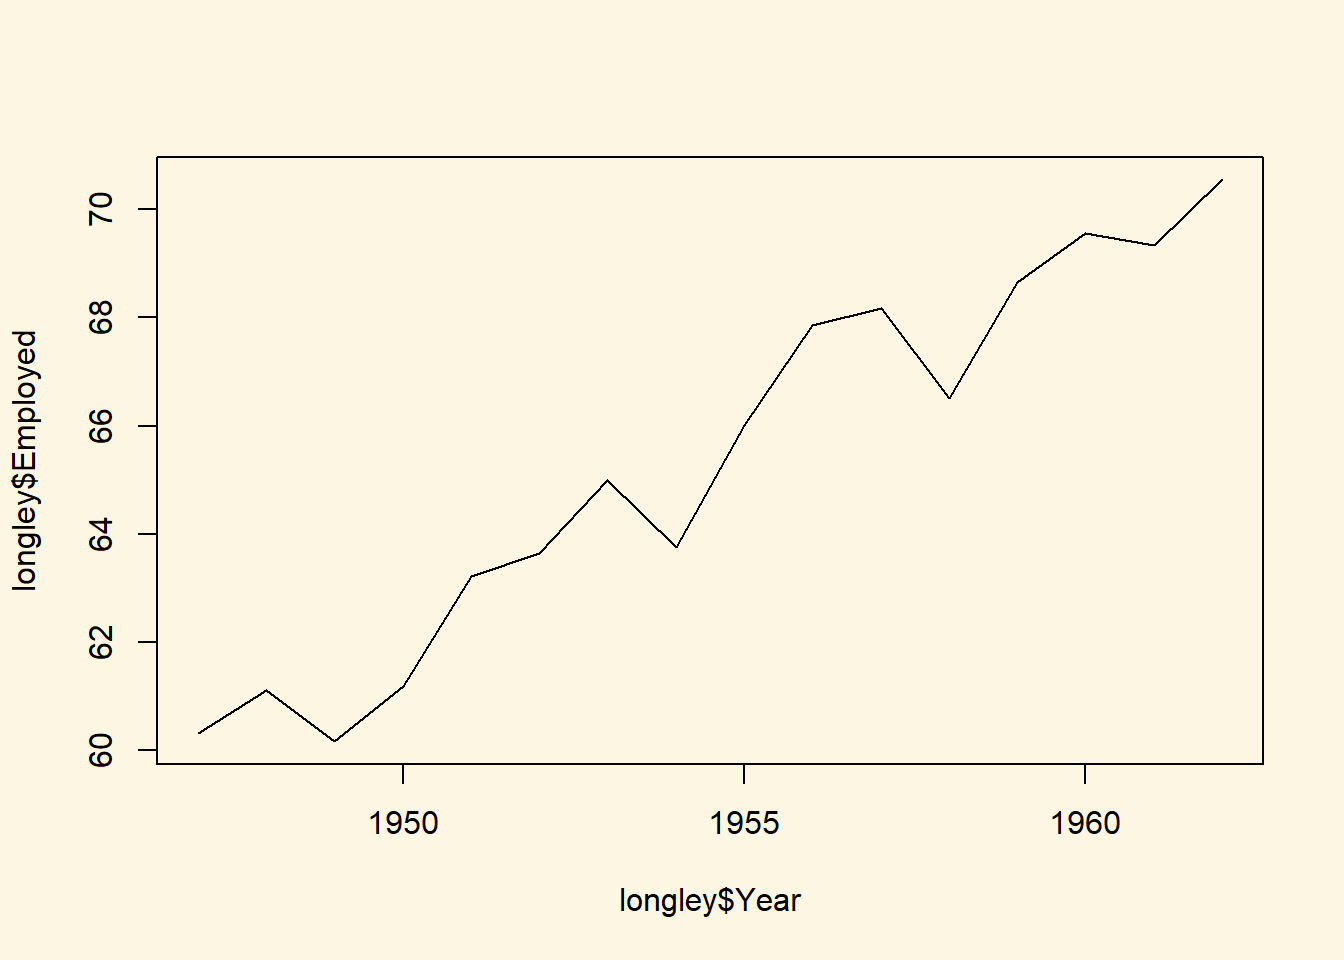
\includegraphics{suffolk2019_files/figure-latex/unnamed-chunk-97-1.pdf}

Create a plot that includes both points and lines.

\begin{Shaded}
\begin{Highlighting}[]
\KeywordTok{plot}\NormalTok{(longley}\OperatorTok{$}\NormalTok{Year, longley}\OperatorTok{$}\NormalTok{Employed, }\DataTypeTok{type =} \StringTok{"b"}\NormalTok{)}
\end{Highlighting}
\end{Shaded}

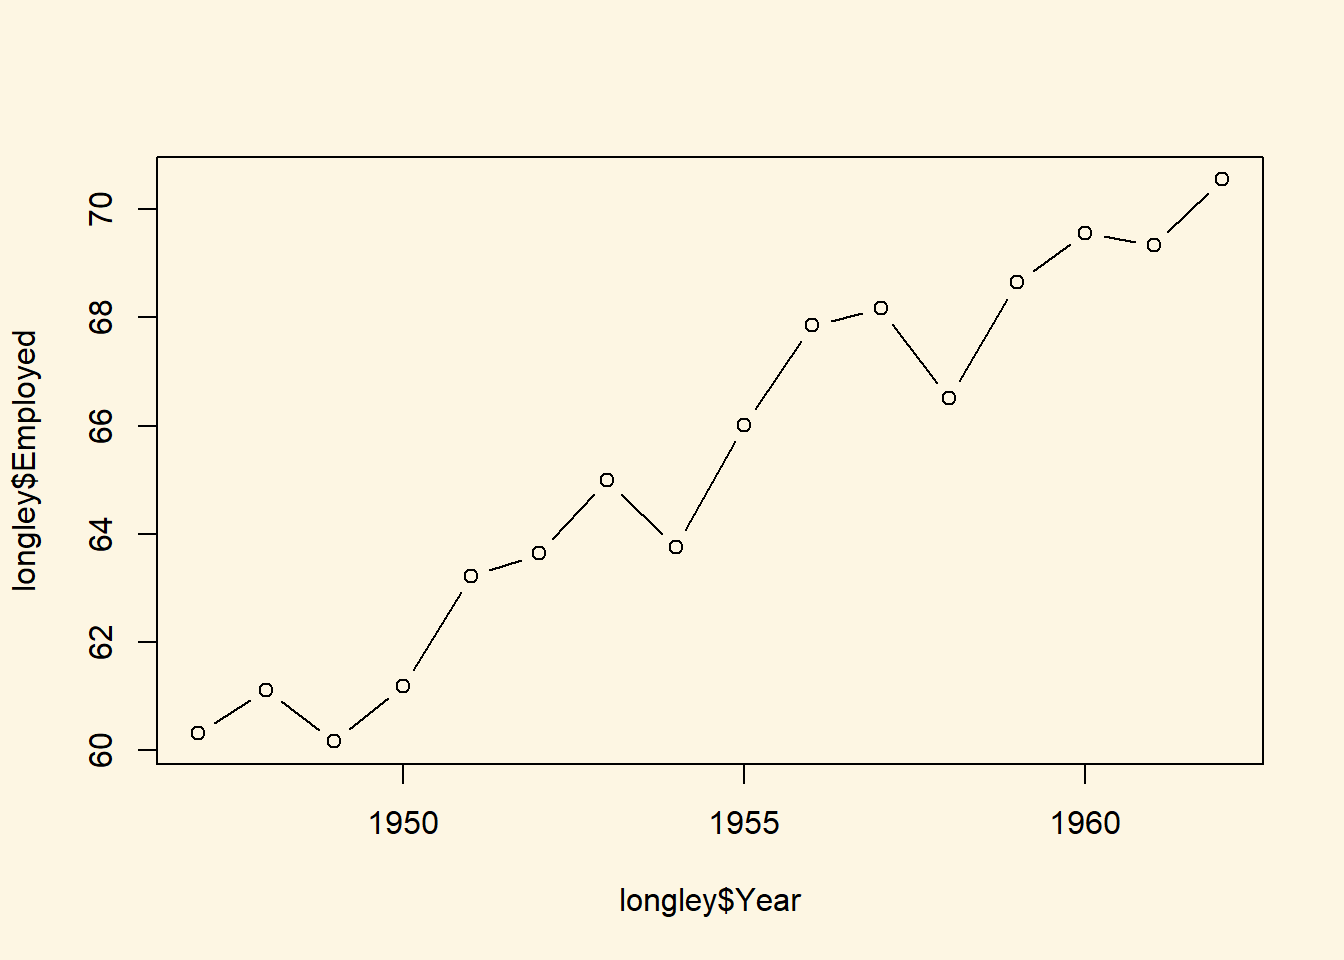
\includegraphics{suffolk2019_files/figure-latex/unnamed-chunk-98-1.pdf}

\hypertarget{correlations-and-differences-in-means}{%
\section{Correlations and differences in means}\label{correlations-and-differences-in-means}}

\hypertarget{seminar-6}{%
\subsection{Seminar}\label{seminar-6}}

In this session, we will cover bi-variate relationships, that is relationships between two variables. For relationships between two continuous variables, we will look at correlations and plots and for relationships between a continuous dependent variable and a binary independent variable, we will look at differences in means.

\hypertarget{sample-variance-and-sample-standard-deviation}{%
\subsubsection{Sample Variance and Sample Standard Deviation}\label{sample-variance-and-sample-standard-deviation}}

The sample variance and sample standard deviation inform us about the degree of variability of our data. Suppose, we were to roll the dice 10 times. We could then compute the mean value that we roll. The sample standard deviation measures by how much an average roll of the dice will deviate from the mean value.

We start rolling the dice, using R's random number generator and the \texttt{runif()} function. The function randomly draws numbers from a uniform distribution. In a uniform distribution each value has the same probability of being drawn. All six sides of a die should be equally likely if the die is fair. Hence, the uniform distribution.

\texttt{runif()} takes three arguments. \texttt{n} is the number of values to be drawn. \texttt{min} is the minimum value and \texttt{max} is the maximum value.

\begin{Shaded}
\begin{Highlighting}[]
\CommentTok{# random draw of 10 values from a uniform distribution}
\NormalTok{dice <-}\StringTok{ }\KeywordTok{runif}\NormalTok{(}\DataTypeTok{n =} \DecValTok{10}\NormalTok{, }\DataTypeTok{min =} \DecValTok{1}\NormalTok{, }\DataTypeTok{max =} \DecValTok{7}\NormalTok{)}
\NormalTok{dice}
\end{Highlighting}
\end{Shaded}

\begin{verbatim}
 [1] 1.741844 5.771283 6.189035 6.244724 4.858865 4.935539 2.975421
 [8] 1.173231 4.266911 6.031508
\end{verbatim}

We have indeed drawn 10 numbers but they are not integers as we would like---we want to simulate a die, so the values should be 1, 2, 3, 4, 5 or 6. We will return to this in a moment but for now let's return to the randomness. Let's draw 10 numbers again:

\begin{Shaded}
\begin{Highlighting}[]
\CommentTok{# random draw of 10 values from a uniform distribution}
\NormalTok{dice2 <-}\StringTok{ }\KeywordTok{runif}\NormalTok{(}\DataTypeTok{n =} \DecValTok{10}\NormalTok{, }\DataTypeTok{min =} \DecValTok{1}\NormalTok{, }\DataTypeTok{max =} \DecValTok{7}\NormalTok{)}

\CommentTok{# first draw}
\NormalTok{dice}
\end{Highlighting}
\end{Shaded}

\begin{verbatim}
 [1] 1.741844 5.771283 6.189035 6.244724 4.858865 4.935539 2.975421
 [8] 1.173231 4.266911 6.031508
\end{verbatim}

\begin{Shaded}
\begin{Highlighting}[]
\CommentTok{# second draw}
\NormalTok{dice2}
\end{Highlighting}
\end{Shaded}

\begin{verbatim}
 [1] 3.835428 6.910071 4.906824 4.243408 2.678436 3.478764 1.262931
 [8] 6.636945 4.675963 6.356551
\end{verbatim}

The numbers of the first and second roll differ because we have drawn values at random. To make our results replicate and to ensure that everyone in the seminar works with the same numbers, we set R's random number generator with the \texttt{set.seed()} function. As argument we plug in some arbitrary value (it does not matter which but using a different one will lead to a different quasi-random draw).

\begin{Shaded}
\begin{Highlighting}[]
\CommentTok{# set random number generator}
\KeywordTok{set.seed}\NormalTok{(}\DecValTok{123}\NormalTok{)}

\CommentTok{# random draw of 10 values from a uniform distribution}
\NormalTok{dice <-}\StringTok{ }\KeywordTok{runif}\NormalTok{(}\DataTypeTok{n =} \DecValTok{10}\NormalTok{, }\DataTypeTok{min =} \DecValTok{1}\NormalTok{, }\DataTypeTok{max =} \DecValTok{7}\NormalTok{)}
\NormalTok{dice}
\end{Highlighting}
\end{Shaded}

\begin{verbatim}
 [1] 2.725465 5.729831 3.453862 6.298104 6.642804 1.273339 4.168633
 [8] 6.354514 4.308610 3.739688
\end{verbatim}

You should all have the same values. If not, run \texttt{set.seed()} again and then do the random draw once. If you do it more than once, the numbers will change. Let's see how this works:

\begin{Shaded}
\begin{Highlighting}[]
\CommentTok{# set random number generator}
\KeywordTok{set.seed}\NormalTok{(}\DecValTok{123}\NormalTok{)}

\CommentTok{# 1st random draw of 10 values from a uniform distribution}
\NormalTok{dice <-}\StringTok{ }\KeywordTok{runif}\NormalTok{(}\DataTypeTok{n =} \DecValTok{10}\NormalTok{, }\DataTypeTok{min =} \DecValTok{1}\NormalTok{, }\DataTypeTok{max =} \DecValTok{7}\NormalTok{)}
\NormalTok{dice}
\end{Highlighting}
\end{Shaded}

\begin{verbatim}
 [1] 2.725465 5.729831 3.453862 6.298104 6.642804 1.273339 4.168633
 [8] 6.354514 4.308610 3.739688
\end{verbatim}

\begin{Shaded}
\begin{Highlighting}[]
\CommentTok{# 2nd random draw of 10 values from a uniform distribution}
\NormalTok{dice2 <-}\StringTok{ }\KeywordTok{runif}\NormalTok{(}\DataTypeTok{n =} \DecValTok{10}\NormalTok{, }\DataTypeTok{min =} \DecValTok{1}\NormalTok{, }\DataTypeTok{max =} \DecValTok{7}\NormalTok{)}
\NormalTok{dice2}
\end{Highlighting}
\end{Shaded}

\begin{verbatim}
 [1] 6.741000 3.720005 5.065424 4.435800 1.617548 6.398950 2.476526
 [8] 1.252357 2.967524 6.727022
\end{verbatim}

\begin{Shaded}
\begin{Highlighting}[]
\CommentTok{# reset random number generator}
\KeywordTok{set.seed}\NormalTok{(}\DecValTok{123}\NormalTok{)}

\CommentTok{# 3rd random draw of 10 values from a uniform distribution}
\NormalTok{dice3 <-}\StringTok{ }\KeywordTok{runif}\NormalTok{(}\DataTypeTok{n =} \DecValTok{10}\NormalTok{, }\DataTypeTok{min =} \DecValTok{1}\NormalTok{, }\DataTypeTok{max =} \DecValTok{7}\NormalTok{)}
\NormalTok{dice3}
\end{Highlighting}
\end{Shaded}

\begin{verbatim}
 [1] 2.725465 5.729831 3.453862 6.298104 6.642804 1.273339 4.168633
 [8] 6.354514 4.308610 3.739688
\end{verbatim}

\begin{Shaded}
\begin{Highlighting}[]
\CommentTok{# 4th random draw of 10 values from a uniform distribution}
\NormalTok{dice4 <-}\StringTok{ }\KeywordTok{runif}\NormalTok{(}\DataTypeTok{n =} \DecValTok{10}\NormalTok{, }\DataTypeTok{min =} \DecValTok{1}\NormalTok{, }\DataTypeTok{max =} \DecValTok{7}\NormalTok{)}
\NormalTok{dice4}
\end{Highlighting}
\end{Shaded}

\begin{verbatim}
 [1] 6.741000 3.720005 5.065424 4.435800 1.617548 6.398950 2.476526
 [8] 1.252357 2.967524 6.727022
\end{verbatim}

As you can see, the the draws from \textbf{dice} and \textbf{dice3} are the same and the draws from \textbf{dice2} and \textbf{dice4} are the same as well. Let's make the values integers with the \texttt{as.integer()} function which simply cuts off all decimal places.

\begin{Shaded}
\begin{Highlighting}[]
\CommentTok{# reset random number generator}
\KeywordTok{set.seed}\NormalTok{(}\DecValTok{123}\NormalTok{)}
\CommentTok{# random draw of 10 numbers from a uniform distribution with minimum 1 and maximum 7}
\NormalTok{dice <-}\StringTok{ }\KeywordTok{runif}\NormalTok{(}\DecValTok{10}\NormalTok{, }\DecValTok{1}\NormalTok{, }\DecValTok{7}\NormalTok{)}
\CommentTok{# cut off decimals places}
\NormalTok{dice <-}\StringTok{ }\KeywordTok{as.integer}\NormalTok{(dice)}
\NormalTok{dice}
\end{Highlighting}
\end{Shaded}

\begin{verbatim}
 [1] 2 5 3 6 6 1 4 6 4 3
\end{verbatim}

\begin{Shaded}
\begin{Highlighting}[]
\CommentTok{# frequency of dice rolls}
\KeywordTok{table}\NormalTok{(dice)}
\end{Highlighting}
\end{Shaded}

\begin{verbatim}
dice
1 2 3 4 5 6 
1 1 2 2 1 3 
\end{verbatim}

We have rolled a six relatively often. All sides should be equally likely but due to sampling variability, we have rolled the six most often. The expected value of a die is 3.5. That is: \[ 1 \times \frac{1}{6} + 2 \times \frac{1}{6} + 3 \times \frac{1}{6} + 4 \times \frac{1}{6} + 5 \times \frac{1}{6} + 6 \times \frac{1}{6} = 3.5\]

We compute the mean in our sample and the standard deviation. Let's start with the mean. Do so yourself.

\begin{Shaded}
\begin{Highlighting}[]
\NormalTok{dice.mean <-}\StringTok{ }\KeywordTok{mean}\NormalTok{(dice)}
\NormalTok{dice.mean}
\end{Highlighting}
\end{Shaded}

\begin{verbatim}
[1] 4
\end{verbatim}

The sample standard deviation tells by how much an average roll of the dice differs from the estimated sample mean. Estimate the sample standard deviation on your own using the \texttt{sd()} function.

\begin{Shaded}
\begin{Highlighting}[]
\NormalTok{std.dev <-}\StringTok{ }\KeywordTok{sd}\NormalTok{(dice)}
\NormalTok{std.dev}
\end{Highlighting}
\end{Shaded}

\begin{verbatim}
[1] 1.763834
\end{verbatim}

An average deviation from the sample mean is 1.76.

\hypertarget{t-test-for-the-sample-mean}{%
\subsubsection{T test for the sample mean}\label{t-test-for-the-sample-mean}}

Our estimate of the mean is 4. The expected value is 3.5. Is this evidence that the die is loaded? The null hypothesis is that the die is fair. The alternative hypothesis is that the die is loaded. Run a t test using the \texttt{t.test()} function. The syntax of the function is:

\begin{verbatim}
t.test(formula, mu, alt, conf)
\end{verbatim}

Lets have a look at the arguments.

\begin{longtable}[]{@{}ll@{}}
\toprule
\begin{minipage}[b]{0.14\columnwidth}\raggedright
Arguments\strut
\end{minipage} & \begin{minipage}[b]{0.80\columnwidth}\raggedright
Description\strut
\end{minipage}\tabularnewline
\midrule
\endhead
\begin{minipage}[t]{0.14\columnwidth}\raggedright
\texttt{formula}\strut
\end{minipage} & \begin{minipage}[t]{0.80\columnwidth}\raggedright
The formula describes the relationship between the dependent and independent variables, for example: • \texttt{dependent.variable\ \textasciitilde{}\ independent.variable}. We will do this in the t-test for the difference in means. Here, we have only one estimated mean. So, we write: • \texttt{variable.name}\strut
\end{minipage}\tabularnewline
\begin{minipage}[t]{0.14\columnwidth}\raggedright
\texttt{mu}\strut
\end{minipage} & \begin{minipage}[t]{0.80\columnwidth}\raggedright
Here, we set the null hypothesis. The null hypothesis is that the true population mean is 10000. Thus, we set \texttt{mu\ =\ 10000}.\strut
\end{minipage}\tabularnewline
\begin{minipage}[t]{0.14\columnwidth}\raggedright
\texttt{alt}\strut
\end{minipage} & \begin{minipage}[t]{0.80\columnwidth}\raggedright
There are two alternatives to the null hypothesis that the difference in means is zero. The difference could either be smaller or it could be larger than zero. To test against both alternatives, we set \texttt{alt\ =\ "two.sided"}.\strut
\end{minipage}\tabularnewline
\begin{minipage}[t]{0.14\columnwidth}\raggedright
\texttt{conf}\strut
\end{minipage} & \begin{minipage}[t]{0.80\columnwidth}\raggedright
Here, we set the level of confidence that we want in rejecting the null hypothesis. Common confidence intervals are: 95\%, 99\%, and 99.9\%.\strut
\end{minipage}\tabularnewline
\bottomrule
\end{longtable}

\begin{Shaded}
\begin{Highlighting}[]
\KeywordTok{t.test}\NormalTok{(dice, }\DataTypeTok{mu =} \FloatTok{3.5}\NormalTok{, }\DataTypeTok{conf.level =} \FloatTok{.95}\NormalTok{, }\DataTypeTok{alt =} \StringTok{"two.sided"}\NormalTok{)}
\end{Highlighting}
\end{Shaded}

\begin{verbatim}

    One Sample t-test

data:  dice
t = 0.89642, df = 9, p-value = 0.3934
alternative hypothesis: true mean is not equal to 3.5
95 percent confidence interval:
 2.738229 5.261771
sample estimates:
mean of x 
        4 
\end{verbatim}

\hypertarget{loading-real-data}{%
\subsubsection{Loading real data}\label{loading-real-data}}

We will load a new dataset from the Quality of Government Institute. The dataset is called \emph{QoG2012.csv}. The codebook follows.

\begin{tabular}{l|l}
\hline
Variable & Description\\
\hline
h\_j & 1 if Free Judiciary\\
\hline
wdi\_gdpc & Per capita wealth in US dollars\\
\hline
undp\_hdi & Human development index (higher values = higher quality of life)\\
\hline
wbgi\_cce & Control of corruption index (higher values = more control of corruption)\\
\hline
wbgi\_pse & Political stability index (higher values = more stable)\\
\hline
former\_col & 1 = country was a colony once\\
\hline
lp\_lat\_abst & Latitude of country's captial divided by 90\\
\hline
\end{tabular}

\begin{Shaded}
\begin{Highlighting}[]
\NormalTok{world.data <-}\StringTok{ }\KeywordTok{read.csv}\NormalTok{(}\StringTok{"QoG2012.csv"}\NormalTok{)}
\end{Highlighting}
\end{Shaded}

Go ahead and load the csv dataset yourself.

\hypertarget{t-test-one-sample-hypothesis-test-with-real-data}{%
\subsubsection{T-test (one-sample hypothesis test) with real data}\label{t-test-one-sample-hypothesis-test-with-real-data}}

A knowledgeable friend declares that worldwide wealth stands at exactly 10 000 US dollars per capita today. We would like to know whether she is right and tease her relentlessly if she isn't.

So, first we take the mean of the wealth variable \texttt{wdi\_gdpc}.

\begin{Shaded}
\begin{Highlighting}[]
\KeywordTok{mean}\NormalTok{(world.data}\OperatorTok{$}\NormalTok{wdi_gdpc)}
\end{Highlighting}
\end{Shaded}

\begin{verbatim}
[1] NA
\end{verbatim}

R returns \texttt{NA} because for some countries we have no reliable information on their per capita wealth. \texttt{NA} means that the data is missing. We can tell the \texttt{mean()} function to estimate the mean only for those countries we have data for, we will, therefore, ignore the countries we do not have information for.

We do so by setting the argument \texttt{na.rm} to TRUE like so: \texttt{mean(dataset\_name\$var\_name,\ na.rm\ =\ TRUE)}.

\begin{Shaded}
\begin{Highlighting}[]
\NormalTok{wealth.mean <-}\StringTok{ }\KeywordTok{mean}\NormalTok{(world.data}\OperatorTok{$}\NormalTok{wdi_gdpc, }\DataTypeTok{na.rm =} \OtherTok{TRUE}\NormalTok{)}
\NormalTok{wealth.mean}
\end{Highlighting}
\end{Shaded}

\begin{verbatim}
[1] 10184.09
\end{verbatim}

Wow, our friend is quite close. Substantially, the difference of our friends claim to our estimate is small but we could still find that the difference is statistically significant (it's a noticeable systematic difference).

Because we do not have information on all countries, our 10184.09 is an estimate and the true population mean -- the population here would be all countries in the world -- may be 10000 as our friend claims. We test this statistically.

In statistics jargon: we would like to test whether our estimate is statistically different from the 10000 figure (the null hypothesis) suggested by our friend. Put differently, we would like to know the probability that we estimate 10184.09 if the true mean of all countries is 10000. This probability is called the p value. Think of the p value of the probability that the relationship that we see, immerged by chance alone. If the p value is low, we can be reasonably confident that the observed relationship did not imerge by chance alone.

We usually compare our p value to a threshold value. That threshold value is called the alpha level and it is the tolerance for false positives. If the p value is less than this value, we speak of a statisically significant relationship. Otherwise, a relationship is insignificant which means we are not confident enought that result is not due to chance.

We must specify our alpha level before we carry out analysis. The acceptable alpha level depends on the quantity of data that you have and how accurartely data is measured. Essentially, the acceptable value is arbitaray. In social sciences the usual threshold value 0.5.

If the p value is less than 0.5, a relationship is significant in our eyes.

We now test whether our estimate is systematically different from the proprosed 10000 figure or not. We do this using the the t-test function \texttt{t.test()}.

\begin{Shaded}
\begin{Highlighting}[]
\KeywordTok{t.test}\NormalTok{(world.data}\OperatorTok{$}\NormalTok{wdi_gdpc, }\DataTypeTok{mu =} \DecValTok{10000}\NormalTok{, }\DataTypeTok{alt =} \StringTok{"two.sided"}\NormalTok{) }
\end{Highlighting}
\end{Shaded}

\begin{verbatim}

    One Sample t-test

data:  world.data$wdi_gdpc
t = 0.19951, df = 177, p-value = 0.8421
alternative hypothesis: true mean is not equal to 10000
95 percent confidence interval:
  8363.113 12005.069
sample estimates:
mean of x 
 10184.09 
\end{verbatim}

The results are similar. Therefore, we can conclude that we are unable to reject the null hypothesis suggested by our friend that the population mean is equal to \texttt{10000}. In statistics jargon, we fail to reject the null hypothesis.

Let's move on to a t-test to test the difference between two estimated means.

\hypertarget{t-test-difference-in-means}{%
\subsubsection{T-test (difference in means)}\label{t-test-difference-in-means}}

We are interested in whether there is a difference in income between countries that have an independent judiciary and countries that do not have an independent judiciary. Put more formally, we are interested in the difference between two conditional means. Recall that a conditional mean is the mean in a subpopulation such as the mean of income given that the country was a victim of colonialization (conditional mean 1).

The t-test is the appropriate test-statistic. Our interval-level dependent variable is \texttt{wdi\_gdpc} which is GDP per capita taken from the World Development Indicators of the World Bank. Our binary independent variable is \texttt{h\_j}.

Let's check the summary statistics of our dependent variable GDP per captia using the \href{https://www.rdocumentation.org/packages/base/versions/3.4.1/topics/summary}{\texttt{summary()}}. It returns several descriptive statistics as well as the number of NA observations (missing values). Missing values mean that we have no information on the correct value of the variable for an observation. Missing values may be missing for many different reasons. We need to be aware of missings because we cannot calculate with missings.

\begin{Shaded}
\begin{Highlighting}[]
\KeywordTok{summary}\NormalTok{(world.data}\OperatorTok{$}\NormalTok{wdi_gdpc)}
\end{Highlighting}
\end{Shaded}

\begin{verbatim}
   Min. 1st Qu.  Median    Mean 3rd Qu.    Max.    NA's 
  226.2  1768.0  5326.1 10184.1 12976.5 63686.7      16 
\end{verbatim}

We use the \texttt{which()} function to identify the row-numbers of the countries in our dataset that have free judiciaries. The code below returns the row index numbers of countries with free judiciaires.

\begin{Shaded}
\begin{Highlighting}[]
\KeywordTok{which}\NormalTok{(world.data}\OperatorTok{$}\NormalTok{h_j }\OperatorTok{==}\StringTok{ }\DecValTok{1}\NormalTok{)}
\end{Highlighting}
\end{Shaded}

\begin{verbatim}
 [1]   9  10  15  16  20  25  31  36  38  43  44  46  47  48  49  55  57
[18]  59  60  65  75  76  77  79  81  82  83  86  88  91  92  97 101 102
[35] 113 114 116 119 122 124 125 128 138 139 143 156 157 158 159 163 167
[52] 168 169 171 174 177 180 181 182 183 184 185 186 194
\end{verbatim}

Now, all we need is to index the dataset like we did yesterday. We access the variable that we want (\texttt{wdi\_gdpc}) with the dollar sign and the rows in square brackets. The code below returns the per capita wealth of the countries with a free judiciary.

\begin{Shaded}
\begin{Highlighting}[]
\KeywordTok{mean}\NormalTok{( world.data}\OperatorTok{$}\NormalTok{wdi_gdpc[}\KeywordTok{which}\NormalTok{(world.data}\OperatorTok{$}\NormalTok{h_j }\OperatorTok{==}\StringTok{ }\DecValTok{1}\NormalTok{)], }\DataTypeTok{na.rm =} \OtherTok{TRUE}\NormalTok{)}
\end{Highlighting}
\end{Shaded}

\begin{verbatim}
[1] 17826.59
\end{verbatim}

Now, go ahead and find the mean per capita wealth of countries with controlled judiciaries yourself.

\begin{Shaded}
\begin{Highlighting}[]
\KeywordTok{mean}\NormalTok{( world.data}\OperatorTok{$}\NormalTok{wdi_gdpc[}\KeywordTok{which}\NormalTok{(world.data}\OperatorTok{$}\NormalTok{h_j }\OperatorTok{==}\StringTok{ }\DecValTok{0}\NormalTok{)], }\DataTypeTok{na.rm =} \OtherTok{TRUE}\NormalTok{)}
\end{Highlighting}
\end{Shaded}

\begin{verbatim}
[1] 5884.882
\end{verbatim}

There is a numeric difference. However, we know that samples are subject to sampling variability. We therefore need to quantify the uncertainty that results from variable samples. To assess whether we can be reasonably sure that the difference between the estimates of wealth is not due to a strage sample but an actual difference in the population, we carry out the t test.

\begin{Shaded}
\begin{Highlighting}[]
\KeywordTok{t.test}\NormalTok{(world.data}\OperatorTok{$}\NormalTok{wdi_gdpc[world.data}\OperatorTok{$}\NormalTok{h_j }\OperatorTok{==}\StringTok{ }\DecValTok{1}\NormalTok{], world.data}\OperatorTok{$}\NormalTok{wdi_gdpc[world.data}\OperatorTok{$}\NormalTok{h_j }\OperatorTok{==}\StringTok{ }\DecValTok{0}\NormalTok{],}
       \DataTypeTok{mu =} \DecValTok{0}\NormalTok{, }\DataTypeTok{alt =} \StringTok{"two.sided"}\NormalTok{, }\DataTypeTok{conf =} \FloatTok{0.95}\NormalTok{)}
\end{Highlighting}
\end{Shaded}

\begin{verbatim}

    Welch Two Sample t-test

data:  world.data$wdi_gdpc[world.data$h_j == 1] and world.data$wdi_gdpc[world.data$h_j == 0]
t = 6.0094, df = 98.261, p-value = 3.165e-08
alternative hypothesis: true difference in means is not equal to 0
95 percent confidence interval:
  7998.36 15885.06
sample estimates:
mean of x mean of y 
17826.591  5884.882 
\end{verbatim}

Let's interpret the results we get from \texttt{t.test()}. The first argument is the vector of wealth values conditional on a free independent judiciary. The second argument is the vector of wealth values conditional on an independent judiciary. The variable of interest is wealth - we call this the dependent variable. We call it dependent because it depends or is conditional on the value of another variable which is the judiciary. We call the conditioning variable, the independent variable.

In our example the question is: Do countries with independent judiciaries have different mean income levels than countries without independent judiciaries?

In the following line you see the t-value, the degrees of freedom and the p-value. Knowing the t-value and the degrees of freedom you can check in a table on t distributions how likely you were to observe this data, if the null-hypothesis was true. The p-value gives you this probability directly. For example, a p-value of 0.02 would mean that the probability of seeing this data given that there is no difference in incomes between countries with and without independent judiciaries \emph{in the population}, is 2\%. Here the p-value is much smaller than this: 3.165e-08 = 0.00000003156!

In the next line you see the 95\% confidence interval because we specified \texttt{conf=0.95}. If you were to take 100 samples and in each you checked the means of the two groups, 95 times the difference in means would be within the interval you see there.

At the very bottom you see the means of the dependent variable by the two groups of the independent variable. These are the means that we estimated above. In our example, you see the mean income levels in countries were the executive has some control over the judiciary, and in countries were the judiciary is independent.

\hypertarget{relationships-between-continuous-variables}{%
\subsubsection{Relationships between continuous variables}\label{relationships-between-continuous-variables}}

The best way to get a sense for the relationship beetween two continuous variables is to do a scatter plot. The human development index measures the quality of life and the World Bank Control of Corruption Index is a measure for the quality if institutions. We want to evaluate whether the two variables are related at all. Here, we could form the hypothesis that better insitutions improve the quality of life of citizens.

To investigate this relationship, we construct a scatterplot.

\begin{Shaded}
\begin{Highlighting}[]
\KeywordTok{plot}\NormalTok{(}
  \DataTypeTok{x =}\NormalTok{ world.data}\OperatorTok{$}\NormalTok{wbgi_cce,}
  \DataTypeTok{y =}\NormalTok{ world.data}\OperatorTok{$}\NormalTok{undp_hdi,}
  \DataTypeTok{xlim =} \KeywordTok{c}\NormalTok{(}\OperatorTok{-}\DecValTok{2}\NormalTok{, }\DecValTok{3}\NormalTok{),}
  \DataTypeTok{ylim =} \KeywordTok{c}\NormalTok{(}\DecValTok{0}\NormalTok{, }\DecValTok{1}\NormalTok{),}
  \DataTypeTok{frame =} \OtherTok{FALSE}\NormalTok{,}
  \DataTypeTok{xlab =} \StringTok{"World Bank Control of Corruption Index"}\NormalTok{,}
  \DataTypeTok{ylab =} \StringTok{"UNDP Human Development Index"}\NormalTok{,}
  \DataTypeTok{main =} \StringTok{"Relationship b/w Quality of Institutions and Quality of Life"}\NormalTok{,}
  \DataTypeTok{pch =} \DecValTok{16}\NormalTok{,}
  \DataTypeTok{col =} \StringTok{"darkgray"}
\NormalTok{)}
\end{Highlighting}
\end{Shaded}

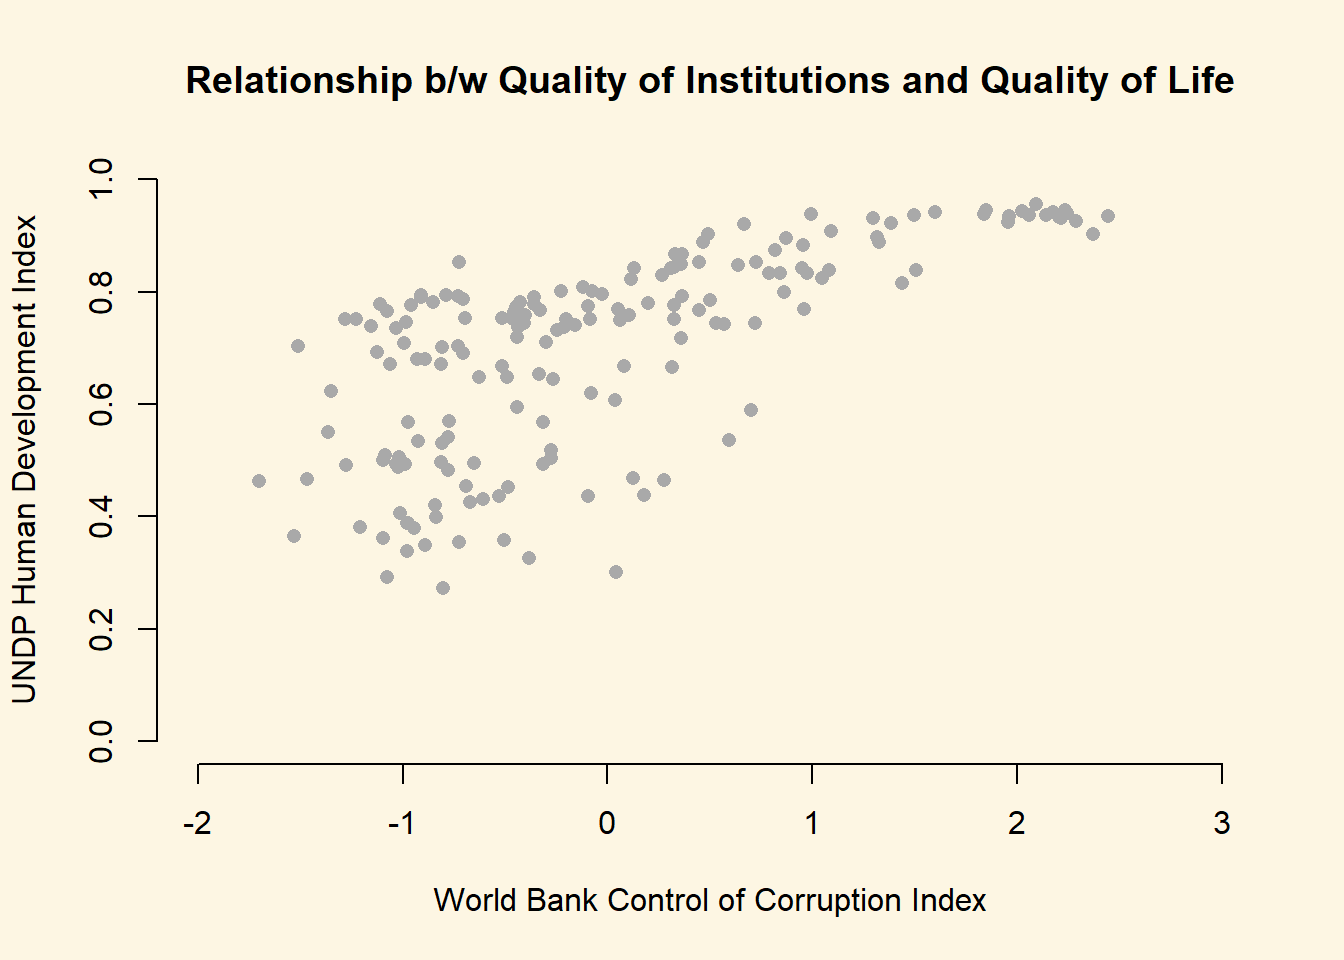
\includegraphics{suffolk2019_files/figure-latex/unnamed-chunk-119-1.pdf}

The plot will give you a good idea whether about whether these two variables are related or not. Sometimes, the correleation coefficient is reported. The correlation coefficient is a measure of \textbf{linear} association. It can take values between -1 and +1. Where -1 is a perfect negative relationship, 0 is a no relationship and +1 is a perfect positive relationship.

While the correlation coefficient is widely used as a summary statistic. Its weakness is that it is a measure of linear association only. That means, there could be a curvilinear realtionship which we miss (for instance a u-shaped relationship). visual inspection using a scatterplot is usually better than estimating the correlation coefficient.

We estimate the correlation coefficient in the following:

\begin{Shaded}
\begin{Highlighting}[]
\KeywordTok{cor}\NormalTok{(}\DataTypeTok{y =}\NormalTok{ world.data}\OperatorTok{$}\NormalTok{undp_hdi, }\DataTypeTok{x =}\NormalTok{ world.data}\OperatorTok{$}\NormalTok{wbgi_cce, }\DataTypeTok{use =} \StringTok{"complete.obs"}\NormalTok{)}
\end{Highlighting}
\end{Shaded}

\begin{verbatim}
[1] 0.6821114
\end{verbatim}

\begin{longtable}[]{@{}ll@{}}
\toprule
\begin{minipage}[b]{0.11\columnwidth}\raggedright
Argument\strut
\end{minipage} & \begin{minipage}[b]{0.83\columnwidth}\raggedright
Description\strut
\end{minipage}\tabularnewline
\midrule
\endhead
\begin{minipage}[t]{0.11\columnwidth}\raggedright
\texttt{x}\strut
\end{minipage} & \begin{minipage}[t]{0.83\columnwidth}\raggedright
The x variable that you want to correlate.\strut
\end{minipage}\tabularnewline
\begin{minipage}[t]{0.11\columnwidth}\raggedright
\texttt{y}\strut
\end{minipage} & \begin{minipage}[t]{0.83\columnwidth}\raggedright
The y variable that you want to correlate.\strut
\end{minipage}\tabularnewline
\begin{minipage}[t]{0.11\columnwidth}\raggedright
\texttt{use}\strut
\end{minipage} & \begin{minipage}[t]{0.83\columnwidth}\raggedright
How R should handle missing values. \texttt{use="complete.obs"} will use only those rows where neither \texttt{x} nor \texttt{y} is missing.\strut
\end{minipage}\tabularnewline
\bottomrule
\end{longtable}

The interpretation of the correlation coefficient is that there is a positive relationship. There is really no threshold value beyond or below which a correlation coefficient is large or small. This depends entirely on the context in this is where your domain knowledge would come in.

\hypertarget{regression}{%
\section{Regression}\label{regression}}

\hypertarget{seminar-7}{%
\subsection{Seminar}\label{seminar-7}}

In this section, we will cover regression models. We will first introduce the bivariate linear regression model. We will then move to linear models with multiple independent variables. Next, we discuss counfounders as threats to our inference. Finally, we will introduce the logistic regression model.

First, however, we install a new pacakge called \texttt{texreg} which makes it easy to produce publication quality output from our regression models. We'll discuss this package in more detail as we go along. For now let's install the package with the \texttt{install.packages("texreg")} function and then load it using \texttt{library(texreg)}.

\begin{Shaded}
\begin{Highlighting}[]
\KeywordTok{install.packages}\NormalTok{(}\StringTok{"texreg"}\NormalTok{)}
\KeywordTok{library}\NormalTok{(texreg)}
\end{Highlighting}
\end{Shaded}

We will use a dataset collected by the US census bureau that contains several socioeconomic indicators.

\begin{Shaded}
\begin{Highlighting}[]
\NormalTok{communities <-}\StringTok{ }\KeywordTok{read.csv}\NormalTok{(}\StringTok{"communities.csv"}\NormalTok{)}
\end{Highlighting}
\end{Shaded}

The dataset includes 38 variables but we're only interested in a handful at the moment.

\begin{tabular}{l|l}
\hline
Variable & Description\\
\hline
PctUnemployed & proportion of citizens in each community who are unemployed\\
\hline
PctNotHSGrad & proportion of citizens in each community who failed to finish high-school\\
\hline
population & proportion of adult population living in cities\\
\hline
\end{tabular}

\begin{verbatim}
  PctUnemployed PctNotHSGrad population
1          0.27         0.18       0.19
2          0.27         0.24       0.00
3          0.36         0.43       0.00
4          0.33         0.25       0.04
5          0.12         0.30       0.01
6          0.10         0.12       0.02
\end{verbatim}

If we summarize these variables with the \texttt{summary()} function, we will see that they are both measured as proportions (they vary between 0 and 1):

\begin{Shaded}
\begin{Highlighting}[]
\KeywordTok{summary}\NormalTok{(communities}\OperatorTok{$}\NormalTok{PctUnemployed)}
\end{Highlighting}
\end{Shaded}

\begin{verbatim}
   Min. 1st Qu.  Median    Mean 3rd Qu.    Max. 
 0.0000  0.2200  0.3200  0.3635  0.4800  1.0000 
\end{verbatim}

\begin{Shaded}
\begin{Highlighting}[]
\KeywordTok{summary}\NormalTok{(communities}\OperatorTok{$}\NormalTok{PctNotHSGrad)}
\end{Highlighting}
\end{Shaded}

\begin{verbatim}
   Min. 1st Qu.  Median    Mean 3rd Qu.    Max. 
 0.0000  0.2300  0.3600  0.3833  0.5100  1.0000 
\end{verbatim}

It will be a little easier to interpret the regression output if we convert these to percentages rather than proportions. We can do this with the following lines of code:

\begin{Shaded}
\begin{Highlighting}[]
\NormalTok{communities}\OperatorTok{$}\NormalTok{PctUnemployed <-}\StringTok{ }\NormalTok{communities}\OperatorTok{$}\NormalTok{PctUnemployed }\OperatorTok{*}\StringTok{ }\DecValTok{100}
\NormalTok{communities}\OperatorTok{$}\NormalTok{PctNotHSGrad <-}\StringTok{ }\NormalTok{communities}\OperatorTok{$}\NormalTok{PctNotHSGrad }\OperatorTok{*}\StringTok{ }\DecValTok{100}
\end{Highlighting}
\end{Shaded}

We can begin by drawing a scatterplot with the percentage of unemployed people on the y-axis and the percentage of adults without high-school education on the x-axis.

\begin{Shaded}
\begin{Highlighting}[]
\KeywordTok{plot}\NormalTok{(}
  \DataTypeTok{x =}\NormalTok{ communities}\OperatorTok{$}\NormalTok{PctNotHSGrad,}
  \DataTypeTok{y =}\NormalTok{ communities}\OperatorTok{$}\NormalTok{PctUnemployed,}
  \DataTypeTok{xlab =} \StringTok{"Adults without high school education (%)"}\NormalTok{,}
  \DataTypeTok{ylab =} \StringTok{"Unemployment (%)"}\NormalTok{,}
  \DataTypeTok{frame.plot =} \OtherTok{FALSE}\NormalTok{,}
  \DataTypeTok{pch =} \DecValTok{20}\NormalTok{,}
  \DataTypeTok{col =} \StringTok{"LightSkyBlue"}
\NormalTok{)}
\end{Highlighting}
\end{Shaded}

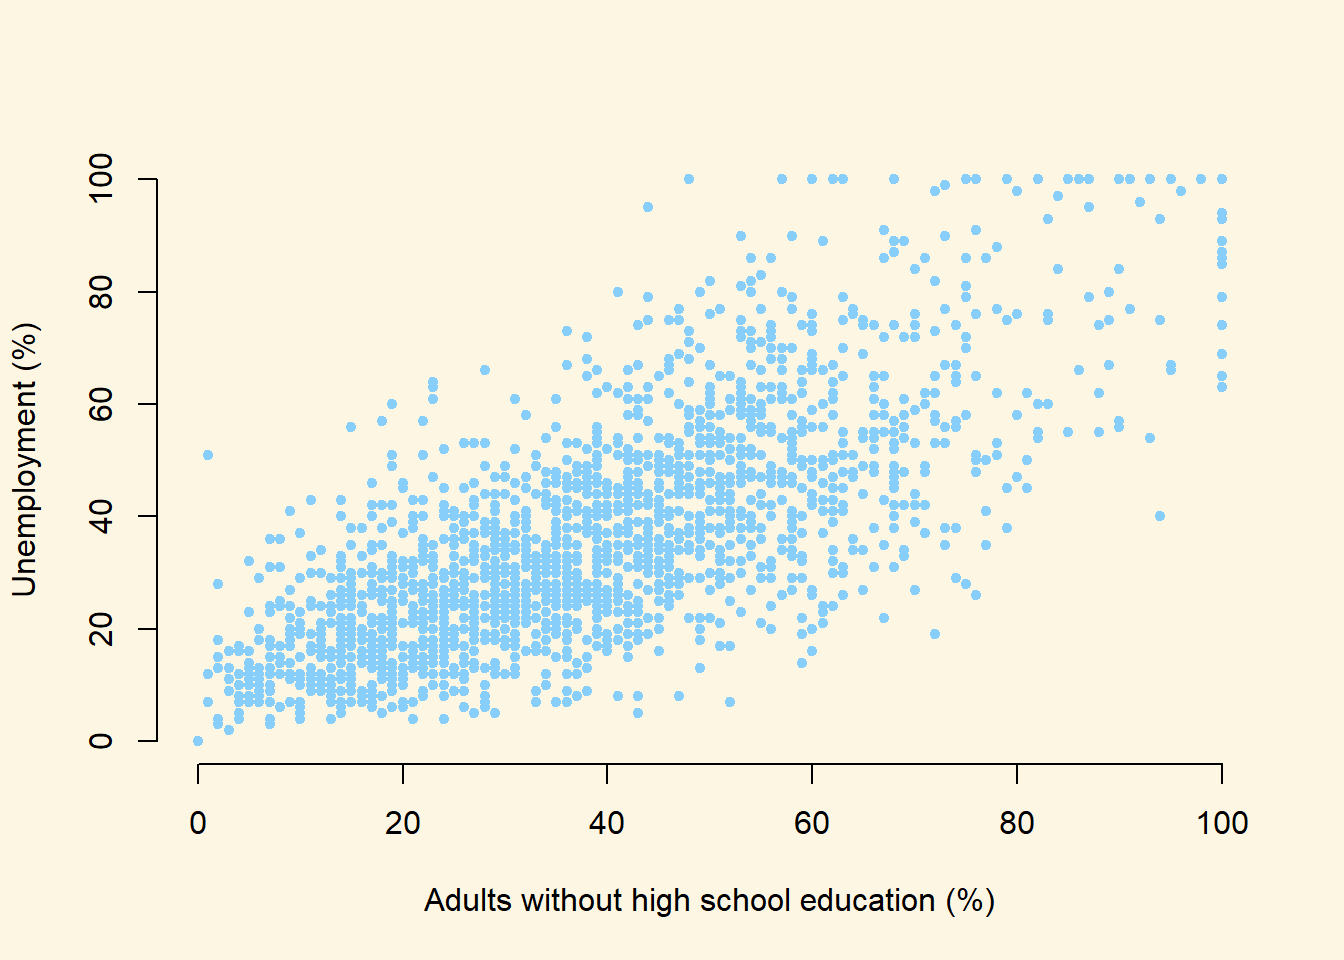
\includegraphics{suffolk2019_files/figure-latex/unnamed-chunk-130-1.pdf}

From looking at the plot, what is the association between the unemployment rate and lack of high-school level education?

In order to answer that question empirically, we will run a linear regression using the \href{http://bit.ly/R_lm}{\texttt{lm()}} function in R. The \href{http://bit.ly/R_lm}{\texttt{lm()}} function needs to know a) the relationship we're trying to model and b) the dataset for our observations. The two arguments we need to provide to the \href{http://bit.ly/R_lm}{\texttt{lm()}} function are described below.

\begin{longtable}[]{@{}ll@{}}
\toprule
\begin{minipage}[b]{0.11\columnwidth}\raggedright
Argument\strut
\end{minipage} & \begin{minipage}[b]{0.83\columnwidth}\raggedright
Description\strut
\end{minipage}\tabularnewline
\midrule
\endhead
\begin{minipage}[t]{0.11\columnwidth}\raggedright
\texttt{formula}\strut
\end{minipage} & \begin{minipage}[t]{0.83\columnwidth}\raggedright
The \texttt{formula} describes the relationship between the dependent and independent variables, for example \texttt{dependent.variable\ \textasciitilde{}\ independent.variable} In our case, we'd like to model the relationship using the formula: \texttt{PctUnemployed\ \textasciitilde{}\ PctNotHSGrad}\strut
\end{minipage}\tabularnewline
\begin{minipage}[t]{0.11\columnwidth}\raggedright
\texttt{data}\strut
\end{minipage} & \begin{minipage}[t]{0.83\columnwidth}\raggedright
This is simply the name of the dataset that contains the variable of interest. In our case, this is the merged dataset called \texttt{communities}.\strut
\end{minipage}\tabularnewline
\bottomrule
\end{longtable}

For more information on how the \texttt{lm()} function works, type help(lm) in R.

\begin{Shaded}
\begin{Highlighting}[]
\NormalTok{model1 <-}\StringTok{ }\KeywordTok{lm}\NormalTok{(PctUnemployed }\OperatorTok{~}\StringTok{ }\NormalTok{PctNotHSGrad, }\DataTypeTok{data =}\NormalTok{ communities)}
\end{Highlighting}
\end{Shaded}

\hypertarget{interpreting-regression-output}{%
\subsubsection{Interpreting Regression Output}\label{interpreting-regression-output}}

The \href{http://bit.ly/R_lm}{\texttt{lm()}} function has modeled the relationship between \texttt{PctUnemployed} and \texttt{PctNotHSGrad} and we've saved it in an object called \texttt{model1}. Let's use the \href{http://bit.ly/R_summary}{\texttt{summary()}} function to see what this linear model looks like.

\begin{Shaded}
\begin{Highlighting}[]
\KeywordTok{summary}\NormalTok{(model1)}
\end{Highlighting}
\end{Shaded}

The output from \href{http://bit.ly/R_summary}{\texttt{summary()}} might seem overwhelming at first so let's break it down one item at a time.

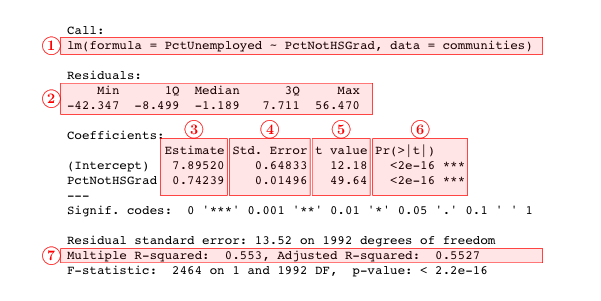
\includegraphics[width=7.29167in,height=\textheight]{img/lm-annotated-1.png}

\begin{longtable}[]{@{}lll@{}}
\toprule
\begin{minipage}[b]{0.07\columnwidth}\raggedright
\#\strut
\end{minipage} & \begin{minipage}[b]{0.21\columnwidth}\raggedright
Item\strut
\end{minipage} & \begin{minipage}[b]{0.63\columnwidth}\raggedright
Description\strut
\end{minipage}\tabularnewline
\midrule
\endhead
\begin{minipage}[t]{0.07\columnwidth}\raggedright
\textbf{1}\strut
\end{minipage} & \begin{minipage}[t]{0.21\columnwidth}\raggedright
\emph{formula}\strut
\end{minipage} & \begin{minipage}[t]{0.63\columnwidth}\raggedright
The \emph{formula} describes the relationship between the dependent and independent variables\strut
\end{minipage}\tabularnewline
\begin{minipage}[t]{0.07\columnwidth}\raggedright
\textbf{2}\strut
\end{minipage} & \begin{minipage}[t]{0.21\columnwidth}\raggedright
\emph{residuals}\strut
\end{minipage} & \begin{minipage}[t]{0.63\columnwidth}\raggedright
The differences between the observed values and the predicted values are called \emph{residuals}.\strut
\end{minipage}\tabularnewline
\begin{minipage}[t]{0.07\columnwidth}\raggedright
\textbf{3}\strut
\end{minipage} & \begin{minipage}[t]{0.21\columnwidth}\raggedright
\emph{coefficients}\strut
\end{minipage} & \begin{minipage}[t]{0.63\columnwidth}\raggedright
The \emph{coefficients} for all the \emph{independent} variables and the intercept. Using the \emph{coefficients} we can write down the relationship between the \emph{dependent} and the \emph{independent} variables as: \texttt{PctUnemployed} = 7.8952023 + ( 0.7423853 * \texttt{PctNotHSGrad} ) This tells us that for each unit increase in the variable \texttt{PctNotHSGrad}, the \texttt{PctUnemployed} increases by 0.7423853.\strut
\end{minipage}\tabularnewline
\begin{minipage}[t]{0.07\columnwidth}\raggedright
\textbf{4}\strut
\end{minipage} & \begin{minipage}[t]{0.21\columnwidth}\raggedright
\emph{standard error}\strut
\end{minipage} & \begin{minipage}[t]{0.63\columnwidth}\raggedright
The \emph{standard error} estimates the standard deviation of the sampling distribution of the coefficients in our model. We can think of the \emph{standard error} as the measure of precision for the estimated coefficients.\strut
\end{minipage}\tabularnewline
\begin{minipage}[t]{0.07\columnwidth}\raggedright
\textbf{5}\strut
\end{minipage} & \begin{minipage}[t]{0.21\columnwidth}\raggedright
\emph{t-statistic}\strut
\end{minipage} & \begin{minipage}[t]{0.63\columnwidth}\raggedright
The \emph{t-statistic} is obtained by dividing the \emph{coefficients} by the \emph{standard error}.\strut
\end{minipage}\tabularnewline
\begin{minipage}[t]{0.07\columnwidth}\raggedright
\textbf{6}\strut
\end{minipage} & \begin{minipage}[t]{0.21\columnwidth}\raggedright
\emph{p-value}\strut
\end{minipage} & \begin{minipage}[t]{0.63\columnwidth}\raggedright
The \emph{p-value} for each of the coefficients in the model. Recall that according to the null hypotheses, the value of the coefficient of interest is zero. The \emph{p-value} tells us whether can can reject the null hypotheses or not.\strut
\end{minipage}\tabularnewline
\begin{minipage}[t]{0.07\columnwidth}\raggedright
\textbf{7}\strut
\end{minipage} & \begin{minipage}[t]{0.21\columnwidth}\raggedright
\(R^2\) and \emph{adj-\(R^2\)}\strut
\end{minipage} & \begin{minipage}[t]{0.63\columnwidth}\raggedright
tell us how much of the variance in our model is accounted for by the \emph{independent} variable. The \emph{adjusted \(R^2\)} is always smaller than \emph{\(R^2\)} as it takes into account the number of \emph{independent} variables and degrees of freedom.\strut
\end{minipage}\tabularnewline
\bottomrule
\end{longtable}

Now let's add a regression line to the scatter plot using the \href{http://bit.ly/R_abline}{\texttt{abline()}} function.

First we run the same \href{http://bit.ly/R_plot}{\texttt{plot()}} function as before, then we overlay a line with \href{http://bit.ly/R_abline}{\texttt{abline()}}:

\begin{Shaded}
\begin{Highlighting}[]
\KeywordTok{plot}\NormalTok{(}
  \DataTypeTok{x =}\NormalTok{ communities}\OperatorTok{$}\NormalTok{PctNotHSGrad,}
  \DataTypeTok{y =}\NormalTok{ communities}\OperatorTok{$}\NormalTok{PctUnemployed,}
  \DataTypeTok{xlab =} \StringTok{"Adults without high school education (%)"}\NormalTok{,}
  \DataTypeTok{ylab =} \StringTok{"Unemployment (%)"}\NormalTok{,}
  \DataTypeTok{frame.plot =} \OtherTok{FALSE}\NormalTok{,}
  \DataTypeTok{pch =} \DecValTok{20}\NormalTok{,}
  \DataTypeTok{col =} \StringTok{"LightSkyBlue"}
\NormalTok{)}

\KeywordTok{abline}\NormalTok{(model1, }\DataTypeTok{lwd =} \DecValTok{3}\NormalTok{, }\DataTypeTok{col =} \StringTok{"red"}\NormalTok{)}
\end{Highlighting}
\end{Shaded}

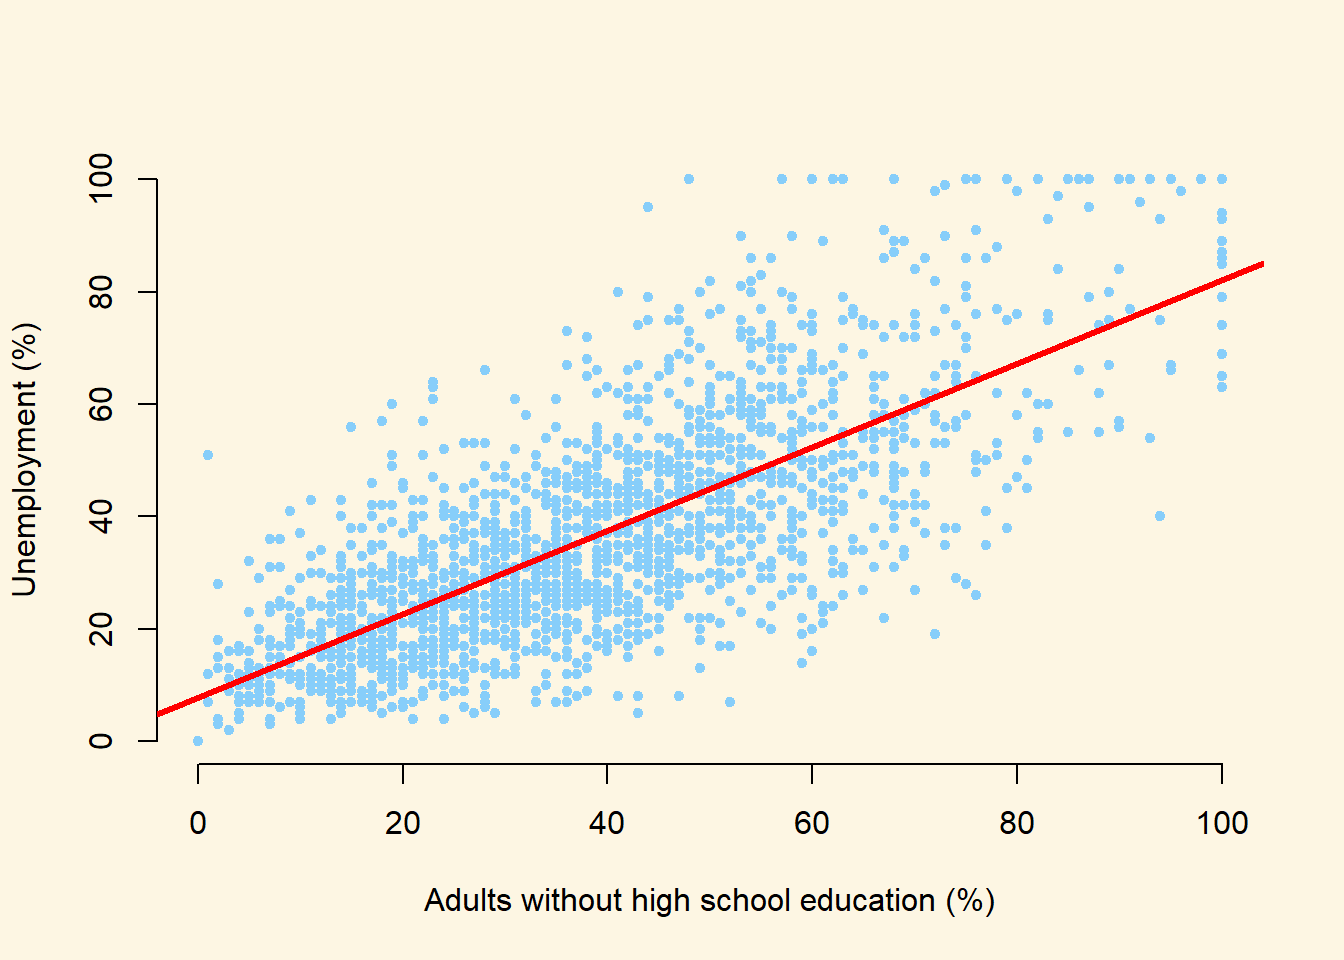
\includegraphics{suffolk2019_files/figure-latex/unnamed-chunk-133-1.pdf}

We can see by looking at the regression line that it matches the coefficients we estimated above. For example, when \texttt{PctNotHSGrad} is equal to zero (i.e.~where the line intersects the Y-axis), the predicted value for \texttt{PctUnemployed} seems to be above 0 but below 10. This is good, as the \emph{intercept} coefficient we estimated in the regression was 7.8952023.

Similarly, the coefficient for the variable \texttt{PctNotHSGrad} was estimated to be 0.7423853, which implies that a one point increase in the percentage of citizens with no high-school education is associated with about 0.7423853 of a point increase in the percentage of citizens who are unemployed. The line in the plot seems to reflect this: it is upward sloping, so that higher levels of the no high-school variable are associated with higher levels of unemployment, but the relationship is not quite 1-to-1. That is, for each additional percentage point of citzens without high school education, the percentage of citizens who are unemployed increases by a little less than one point.

While the \href{http://bit.ly/R_summary}{\texttt{summary()}} function provides a slew of information about a fitted regression model, we often need to present our findings in easy to read tables similar to what you see in journal publications. The \texttt{texreg} package we loaded earlier allows us to do just that.

Let's take a look at how to display the output of a regression model on the screen using the \href{http://bit.ly/R_texreg}{\texttt{screenreg()}} function from \texttt{texreg}.

\begin{Shaded}
\begin{Highlighting}[]
\KeywordTok{screenreg}\NormalTok{(model1)}
\end{Highlighting}
\end{Shaded}

\begin{verbatim}

=========================
              Model 1    
-------------------------
(Intercept)      7.90 ***
                (0.65)   
PctNotHSGrad     0.74 ***
                (0.01)   
-------------------------
R^2              0.55    
Adj. R^2         0.55    
Num. obs.     1994       
RMSE            13.52    
=========================
*** p < 0.001, ** p < 0.01, * p < 0.05
\end{verbatim}

Here, the output includes some of the most salient details we need for interpretation. We can see the coefficient for the \texttt{PctNotHSGrad} variable, and the estimated coefficient for the intercept. Below these numbers, in brackets, we can see the standard errors. The table also reports the \(R^2\), the adjusted \(R^2\), the number of observations (\(n\)) and the root-mean-squared-error (\(RMSE\)).

One thing to note is that the table does not include either t-statistics or p-values for the estimated coefficents. Instead, the table employs a common device of using stars to denote whether a variable is statistically significant at a given alpha level.

\begin{itemize}
\tightlist
\item
  \texttt{***} indicates that the coefficient is significant at the 99.9\% confidence level (alpha = 0.001)
\item
  \texttt{**} indicates that the coefficient is significant at the 99\% confidence level (alpha = 0.01)
\item
  \texttt{*} indicates that the coefficient is significant at the 95\% confidence level (alpha = 0.05)
\end{itemize}

Returning to our example, are there other variables that might affect the unemployment rate in our dataset? For example, is the unemployment rate higher in rural areas? To answer this question, we can swap \texttt{PctNotHSGrad} for a different independent variable. Let's use the variable \texttt{population}, which measures the proportion of adults who live in cities (rather than rural areas). Again, we can transform this proportion to a percentage with the following code:

\begin{Shaded}
\begin{Highlighting}[]
\NormalTok{communities}\OperatorTok{$}\NormalTok{population <-}\StringTok{ }\NormalTok{communities}\OperatorTok{$}\NormalTok{population }\OperatorTok{*}\StringTok{ }\DecValTok{100}
\end{Highlighting}
\end{Shaded}

Let's fit a linear model using \texttt{population} as the independent variable:

\begin{Shaded}
\begin{Highlighting}[]
\NormalTok{model2 <-}\StringTok{ }\KeywordTok{lm}\NormalTok{(PctUnemployed }\OperatorTok{~}\StringTok{ }\NormalTok{population, }\DataTypeTok{data =}\NormalTok{ communities)}
\KeywordTok{summary}\NormalTok{(model2)}
\end{Highlighting}
\end{Shaded}

\begin{verbatim}

Call:
lm(formula = PctUnemployed ~ population, data = communities)

Residuals:
    Min      1Q  Median      3Q     Max 
-35.252 -14.715  -3.946  11.054  64.980 

Coefficients:
            Estimate Std. Error t value Pr(>|t|)    
(Intercept) 35.02042    0.49206  71.171  < 2e-16 ***
population   0.23139    0.03532   6.552  7.2e-11 ***
---
Signif. codes:  0 '***' 0.001 '**' 0.01 '*' 0.05 '.' 0.1 ' ' 1

Residual standard error: 20.01 on 1992 degrees of freedom
Multiple R-squared:  0.0211,    Adjusted R-squared:  0.02061 
F-statistic: 42.93 on 1 and 1992 DF,  p-value: 7.201e-11
\end{verbatim}

We can show regression line from the \texttt{model2} just like we did with our first model.

\begin{Shaded}
\begin{Highlighting}[]
\KeywordTok{plot}\NormalTok{(}
  \DataTypeTok{x =}\NormalTok{ communities}\OperatorTok{$}\NormalTok{population,}
  \DataTypeTok{y =}\NormalTok{ communities}\OperatorTok{$}\NormalTok{PctUnemployed,}
  \DataTypeTok{xlab =} \StringTok{"Adults living in cities (%)"}\NormalTok{,}
  \DataTypeTok{ylab =} \StringTok{"Unemployment (%)"}\NormalTok{,}
  \DataTypeTok{frame.plot =} \OtherTok{FALSE}\NormalTok{,}
  \DataTypeTok{pch =} \DecValTok{20}\NormalTok{,}
  \DataTypeTok{col =} \StringTok{"LightSkyBlue"}
\NormalTok{)}

\KeywordTok{abline}\NormalTok{(model2, }\DataTypeTok{lwd =} \DecValTok{2}\NormalTok{, }\DataTypeTok{col =} \StringTok{"red"}\NormalTok{)}
\end{Highlighting}
\end{Shaded}

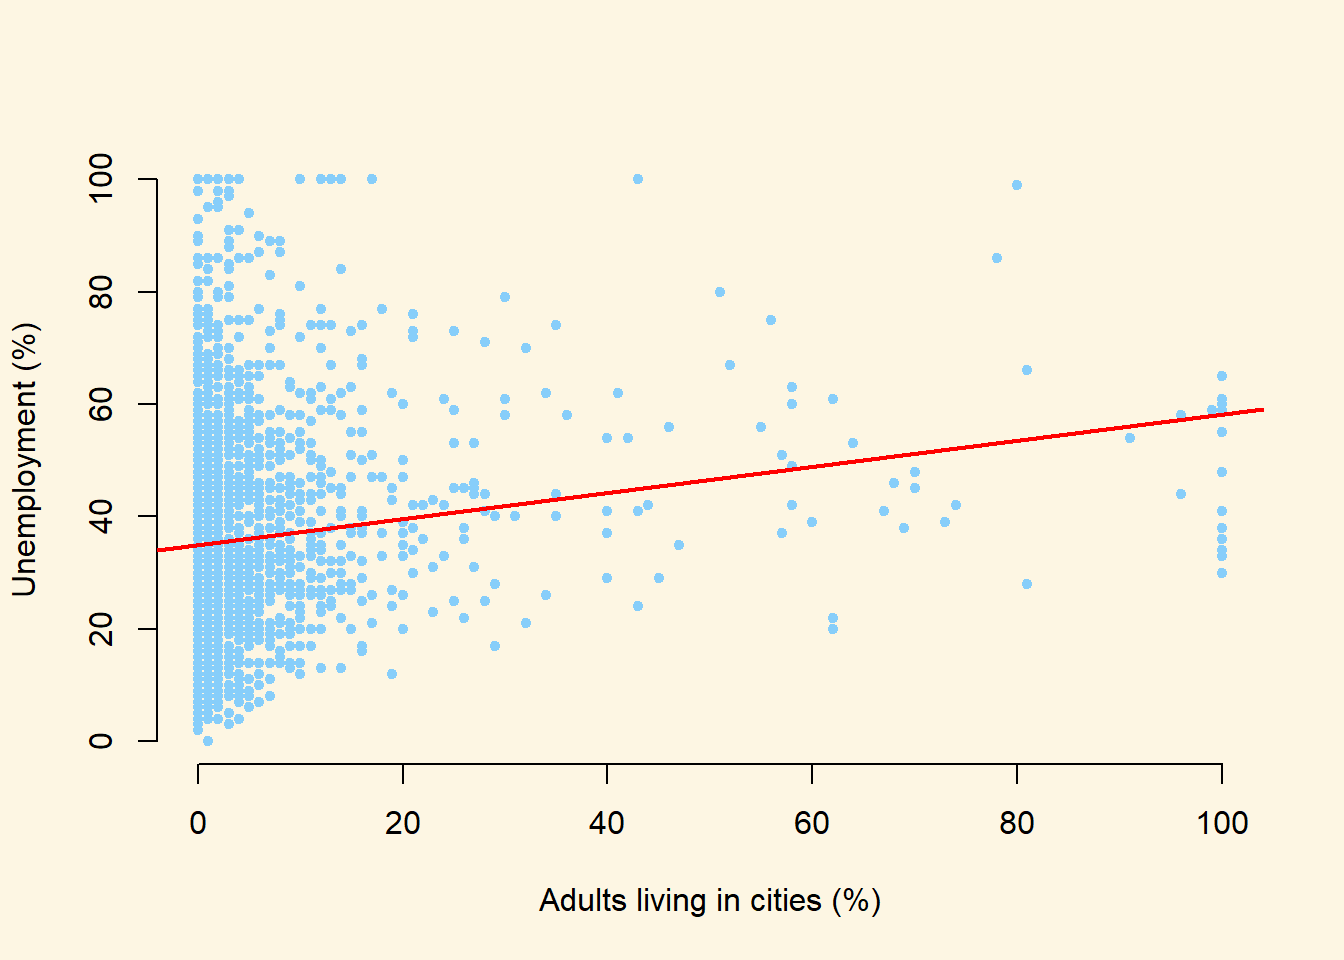
\includegraphics{suffolk2019_files/figure-latex/unnamed-chunk-137-1.pdf}

So we now have two models! Often, we will want to compare two estimated models side-by-side. We might want to say how the coefficients for the independent variables we included differ in \texttt{model1} and \texttt{model2}, for example. Or we may want to ask: Does \texttt{model2} offer a better fit than \texttt{model1}?

It is often useful to print the salient details from the estimated models side-by-side. We can do this by using the \href{http://bit.ly/R_texreg}{\texttt{screenreg()}} function.

\begin{Shaded}
\begin{Highlighting}[]
\KeywordTok{screenreg}\NormalTok{(}\KeywordTok{list}\NormalTok{(model1, model2))}
\end{Highlighting}
\end{Shaded}

\begin{verbatim}

======================================
              Model 1      Model 2    
--------------------------------------
(Intercept)      7.90 ***    35.02 ***
                (0.65)       (0.49)   
PctNotHSGrad     0.74 ***             
                (0.01)                
population                    0.23 ***
                             (0.04)   
--------------------------------------
R^2              0.55         0.02    
Adj. R^2         0.55         0.02    
Num. obs.     1994         1994       
RMSE            13.52        20.01    
======================================
*** p < 0.001, ** p < 0.01, * p < 0.05
\end{verbatim}

What does this table tell us?

\begin{itemize}
\tightlist
\item
  The first column replicates the results from our first model. We can see that a one point increase in the percentage of citizens without high-school education is associated with an increase of 0.7423853 percentage points of unemployment, on average.
\item
  The second column gives us the results from the second model. Here, a one point increase in the percentage of citizens who live in cities is associated with an increase of 0.2313906 percentage points of unemployment, on average
\item
  We can also compare the \(R^2\) values from the two models. The \(R^2\) for \texttt{model1} is 0.5529732 and for \texttt{model2} is 0.0210968. This suggests that the model with \texttt{PctNotHSGrad} as the explanatory variable explains about 55.2973193\% of the variation in unemployment. The model with \texttt{population} as the explanatory variable, on the other hand, explains just 2.1096753\% of the variation in unemployment.
\end{itemize}

Finally, and this is something that might help with your coursework, let's save the same output as a Microsoft Word document using \href{http://bit.ly/R_texreg}{\texttt{htmlreg()}}.

\begin{Shaded}
\begin{Highlighting}[]
\KeywordTok{htmlreg}\NormalTok{(}\KeywordTok{list}\NormalTok{(model1, model2), }\DataTypeTok{file =} \StringTok{"regression_model.doc"}\NormalTok{)}
\end{Highlighting}
\end{Shaded}

If you're using a Mac, you might want to save the file as \texttt{.html} if the Word document isn't formatted correctly.

\begin{Shaded}
\begin{Highlighting}[]
\KeywordTok{htmlreg}\NormalTok{(}\KeywordTok{list}\NormalTok{(model1, model2), }\DataTypeTok{file =} \StringTok{"regression_model.html"}\NormalTok{)}
\end{Highlighting}
\end{Shaded}

\hypertarget{fitted-values}{%
\subsubsection{Fitted values}\label{fitted-values}}

Once we have estimated a regression model, we can use that model to produce fitted values. Fitted values represent our ``best guess'' for the value of our dependent variable for a specific value of our independent variable.

Let's calculate the fitted values manually and then we'll show you how to do it in R. The fitted value formula is:

\[\hat{Y}_{i} = \hat{\beta}_0 + \hat{\beta}_1 * X_i\]

Let's say that, on the basis of \texttt{model1} we would like to know what the unemployment rate is likely to be for a community where the percentage of adults without a high-school education is equal to 10\%. We can substitute in the relevant coefficients from \texttt{model1} and the value for our X variable (\texttt{10} in this case), and we get:

\[\hat{Y}_{i} = 7.9 + 0.74 * 10 = 15.3\]

To calculate fitted values in R, we use the \texttt{predict()} function.

The predict function takes two main arguments.

\begin{longtable}[]{@{}ll@{}}
\toprule
\begin{minipage}[b]{0.11\columnwidth}\raggedright
Argument\strut
\end{minipage} & \begin{minipage}[b]{0.83\columnwidth}\raggedright
Description\strut
\end{minipage}\tabularnewline
\midrule
\endhead
\begin{minipage}[t]{0.11\columnwidth}\raggedright
\texttt{object}\strut
\end{minipage} & \begin{minipage}[t]{0.83\columnwidth}\raggedright
The \texttt{object} is the model object that we would like to use to produce fitted values. Here, we would like to base the analysis on \texttt{model1} and so specify \texttt{object\ =\ model1} here.\strut
\end{minipage}\tabularnewline
\begin{minipage}[t]{0.11\columnwidth}\raggedright
\texttt{newdata}\strut
\end{minipage} & \begin{minipage}[t]{0.83\columnwidth}\raggedright
This is an optional argument which we use to specify the values of our independent variable(s) that we would like fitted values for. If we leave this argument empty, R will automatically calculate fitted values for all of the observations in the data that we used to estimate the original model. If we include this argument, we need to provide a \texttt{data.frame} which has a variable with the same name as the independent variable in our model. Here, we specify \texttt{newdata\ =\ data.frame(PctNotHSGrad\ =\ 10)}, as we would like the fitted value for a community where 10\% of adults did not complete high-school.\strut
\end{minipage}\tabularnewline
\bottomrule
\end{longtable}

\begin{Shaded}
\begin{Highlighting}[]
\KeywordTok{predict}\NormalTok{(model1, }\DataTypeTok{newdata =} \KeywordTok{data.frame}\NormalTok{(}\DataTypeTok{PctNotHSGrad =} \DecValTok{10}\NormalTok{))}
\end{Highlighting}
\end{Shaded}

\begin{verbatim}
       1 
15.31906 
\end{verbatim}

This is the same as the result we obtained when we calculated the fitted value manually. The good thing about the \texttt{predict()} function, however, is that we will be able to use it for \emph{all} the models we study on this course, and it can be useful for calculating many different fitted values.

\hypertarget{additional-resources}{%
\subsubsection{Additional Resources}\label{additional-resources}}

\begin{itemize}
\tightlist
\item
  \href{http://altaf.shinyapps.io/linear-regression}{Linear Regression - Interactive App}
\end{itemize}

\hypertarget{multiple-linear-regression-models}{%
\subsubsection{Multiple linear regression models}\label{multiple-linear-regression-models}}

we load the full standard (cross-sectional) dataset from the Quality of Government Institute (this is a newer version that the one we used earlier). This is a great data source for comparativist research. The codebook is available from their main \href{http://qog.pol.gu.se/data/datadownloads/qogstandarddata}{website}. You can also find time-series and cross-section data sets on this page.

The dataset is in csv format (\texttt{.csv}). Loading it requires the \texttt{read.csv()} function. Let's load the data set.

\begin{Shaded}
\begin{Highlighting}[]
\NormalTok{world_data <-}\StringTok{ }\KeywordTok{read.csv}\NormalTok{(}\StringTok{"http://uclspp.github.io/datasets/data/qog_std_cs_jan15.csv"}\NormalTok{, }\DataTypeTok{stringsAsFactors =} \OtherTok{FALSE}\NormalTok{)}
\end{Highlighting}
\end{Shaded}

Check the dimensions of the dataset

\begin{Shaded}
\begin{Highlighting}[]
\KeywordTok{dim}\NormalTok{(world_data)}
\end{Highlighting}
\end{Shaded}

\begin{verbatim}
[1]  193 2037
\end{verbatim}

The dataset contains 2037 variables but we're only interested in the following:

\begin{tabular}{l|l}
\hline
Variable & Description\\
\hline
wbgi\_pse & A measure of political stability (larger values mean more stability)\\
\hline
lp\_lat\_abst & Distance to the equator or latitude\\
\hline
dr\_ing & Index for the level of globalization\\
\hline
ti\_cpi & Transparency International's Corruptions Perceptions Index (larger values mean better quality institutions, i.e. less corruption)\\
\hline
br\_dem & Factor variable stating whether the country is a democracy or not (with labels `1. Democracy` and `0. Dictatorship`)\\
\hline
\end{tabular}

Our dependent variable (also called response or outcome variable) is \texttt{wbgi\_pse}. We will rename the variables we care about to something meaningful.

CAUTION: When renaming variables, do not use spaces or special characters in the name. You can, however, use a period (\texttt{.}) or underscore (\texttt{\_}) to make the names more readable.

\begin{Shaded}
\begin{Highlighting}[]
\KeywordTok{names}\NormalTok{(world_data)[}\KeywordTok{names}\NormalTok{(world_data) }\OperatorTok{==}\StringTok{ "cname"}\NormalTok{] <-}\StringTok{ "country"}
\KeywordTok{names}\NormalTok{(world_data)[}\KeywordTok{names}\NormalTok{(world_data) }\OperatorTok{==}\StringTok{ "wbgi_pse"}\NormalTok{] <-}\StringTok{ "pol_stability"}
\KeywordTok{names}\NormalTok{(world_data)[}\KeywordTok{names}\NormalTok{(world_data) }\OperatorTok{==}\StringTok{ "lp_lat_abst"}\NormalTok{] <-}\StringTok{ "latitude"}
\KeywordTok{names}\NormalTok{(world_data)[}\KeywordTok{names}\NormalTok{(world_data) }\OperatorTok{==}\StringTok{ "dr_ig"}\NormalTok{] <-}\StringTok{ "globalization"}
\KeywordTok{names}\NormalTok{(world_data)[}\KeywordTok{names}\NormalTok{(world_data) }\OperatorTok{==}\StringTok{ "chga_demo"}\NormalTok{] <-}\StringTok{ "democracy"}
\KeywordTok{names}\NormalTok{(world_data)[}\KeywordTok{names}\NormalTok{(world_data) }\OperatorTok{==}\StringTok{ "ti_cpi"}\NormalTok{] <-}\StringTok{ "inst_quality"}
\end{Highlighting}
\end{Shaded}

Now Let's look at some of these variables using the \texttt{summary()} function.

\begin{Shaded}
\begin{Highlighting}[]
\KeywordTok{summary}\NormalTok{(world_data}\OperatorTok{$}\NormalTok{pol_stability)}
\end{Highlighting}
\end{Shaded}

\begin{verbatim}
    Min.  1st Qu.   Median     Mean  3rd Qu.     Max. 
-3.10637 -0.72686 -0.01900 -0.06079  0.78486  1.57240 
\end{verbatim}

If you think about political stability, and how one could measure it, you know there is an order implicit in the measurement -- more or less stability. From there, what you need to know is whether the more or less is ordinal or interval scaled. Checking \texttt{pol\_stability} you see a range from roughly -3 to 1.6. The variable is numerical and has decimal places. This tells you that the variable is at least interval scaled. You will not see ordinally scaled variables with decimal places. Examine the summaries of the other variables and determine their level of measurement.

Now let's look at the variables that we think can explain political stability. We can use the \texttt{summary()} function on more than one variable by combining their names in a vector.

\begin{Shaded}
\begin{Highlighting}[]
\KeywordTok{summary}\NormalTok{(world_data[}\KeywordTok{c}\NormalTok{(}\StringTok{'latitude'}\NormalTok{, }\StringTok{'globalization'}\NormalTok{, }\StringTok{'inst_quality'}\NormalTok{, }\StringTok{'democracy'}\NormalTok{)])}
\end{Highlighting}
\end{Shaded}

\begin{verbatim}
    latitude      globalization    inst_quality    democracy        
 Min.   :0.0000   Min.   :24.35   Min.   :1.010   Length:193        
 1st Qu.:0.1444   1st Qu.:45.22   1st Qu.:2.400   Class :character  
 Median :0.2444   Median :54.99   Median :3.300   Mode  :character  
 Mean   :0.2865   Mean   :57.15   Mean   :3.988                     
 3rd Qu.:0.4444   3rd Qu.:68.34   3rd Qu.:5.100                     
 Max.   :0.7222   Max.   :92.30   Max.   :9.300                     
 NA's   :12       NA's   :12      NA's   :12                        
\end{verbatim}

The variables \texttt{latitude}, \texttt{globalization} and \texttt{inst\_quality} have 12 missing values each marked as \texttt{NA}. \texttt{democracy} has 1 missing value. Missing values could cause trouble because operations including an \texttt{NA} will produce \texttt{NA} as a result (e.g.: \texttt{1\ +\ NA\ =\ NA}). We will drop these missing values from our data set using the \texttt{is.na()} function and square brackets. The exlamation mark in front of \texttt{is.na()} means ``not''. So, we keep all rows that are not NA's on the variable \texttt{latitude}.

\begin{Shaded}
\begin{Highlighting}[]
\NormalTok{world_data <-}\StringTok{ }\NormalTok{world_data[ }\OperatorTok{!}\KeywordTok{is.na}\NormalTok{(world_data}\OperatorTok{$}\NormalTok{latitude), ]}
\end{Highlighting}
\end{Shaded}

Generally, we want to make sure we drop missing values only from variables that we care about. Now that you have seen how to do this, drop missings from \texttt{globalization}, \texttt{inst\_quality}, and \texttt{democracy} yourself.

\begin{Shaded}
\begin{Highlighting}[]
\NormalTok{world_data <-}\StringTok{ }\NormalTok{world_data[ }\OperatorTok{!}\KeywordTok{is.na}\NormalTok{(world_data}\OperatorTok{$}\NormalTok{globalization), ]}
\NormalTok{world_data <-}\StringTok{ }\NormalTok{world_data[ }\OperatorTok{!}\KeywordTok{is.na}\NormalTok{(world_data}\OperatorTok{$}\NormalTok{inst_quality), ]}
\NormalTok{world_data <-}\StringTok{ }\NormalTok{world_data[ }\OperatorTok{!}\KeywordTok{is.na}\NormalTok{(world_data}\OperatorTok{$}\NormalTok{democracy), ]}
\end{Highlighting}
\end{Shaded}

Let's check the range of the variable \texttt{latitude} from our summary above. It is between \texttt{0} and \texttt{1}. The codebook clarifies that the latitude of a country's capital has been divided by \texttt{90} to get a variable that ranges from \texttt{0} to \texttt{1}. This would make interpretation difficult. When interpreting the effect of such a variable a unit change (a change of \texttt{1}) covers the entire range or put differently, it is a change from a country at the equator to a country at one of the poles.

We therefore multiply by \texttt{90} again. This will turn the units of the \texttt{latitude} variable into degrees again which makes interpretation easier.

\begin{Shaded}
\begin{Highlighting}[]
\NormalTok{world_data}\OperatorTok{$}\NormalTok{latitude <-}\StringTok{ }\NormalTok{world_data}\OperatorTok{$}\NormalTok{latitude }\OperatorTok{*}\StringTok{ }\DecValTok{90}
\end{Highlighting}
\end{Shaded}

\hypertarget{estimating-a-bivariate-regression}{%
\subsubsection{Estimating a Bivariate Regression}\label{estimating-a-bivariate-regression}}

Is there a correlation between the distance of a country to the equator and the level of political stability? Both political stability (dependent variable) and distance to the equator (independent variable) are continuous. Therefore, we will get an idea about the relationship using a scatter plot.

\begin{Shaded}
\begin{Highlighting}[]
\KeywordTok{plot}\NormalTok{(}\DataTypeTok{x =}\NormalTok{ world_data}\OperatorTok{$}\NormalTok{latitude,}
     \DataTypeTok{y =}\NormalTok{ world_data}\OperatorTok{$}\NormalTok{pol_stability, }
     \DataTypeTok{frame.plot =} \OtherTok{FALSE}\NormalTok{,}
     \DataTypeTok{pch =} \DecValTok{20}\NormalTok{,}
     \DataTypeTok{xlab =} \StringTok{"Latitude"}\NormalTok{,}
     \DataTypeTok{ylab =} \StringTok{"Political Stability"}\NormalTok{)}
\end{Highlighting}
\end{Shaded}

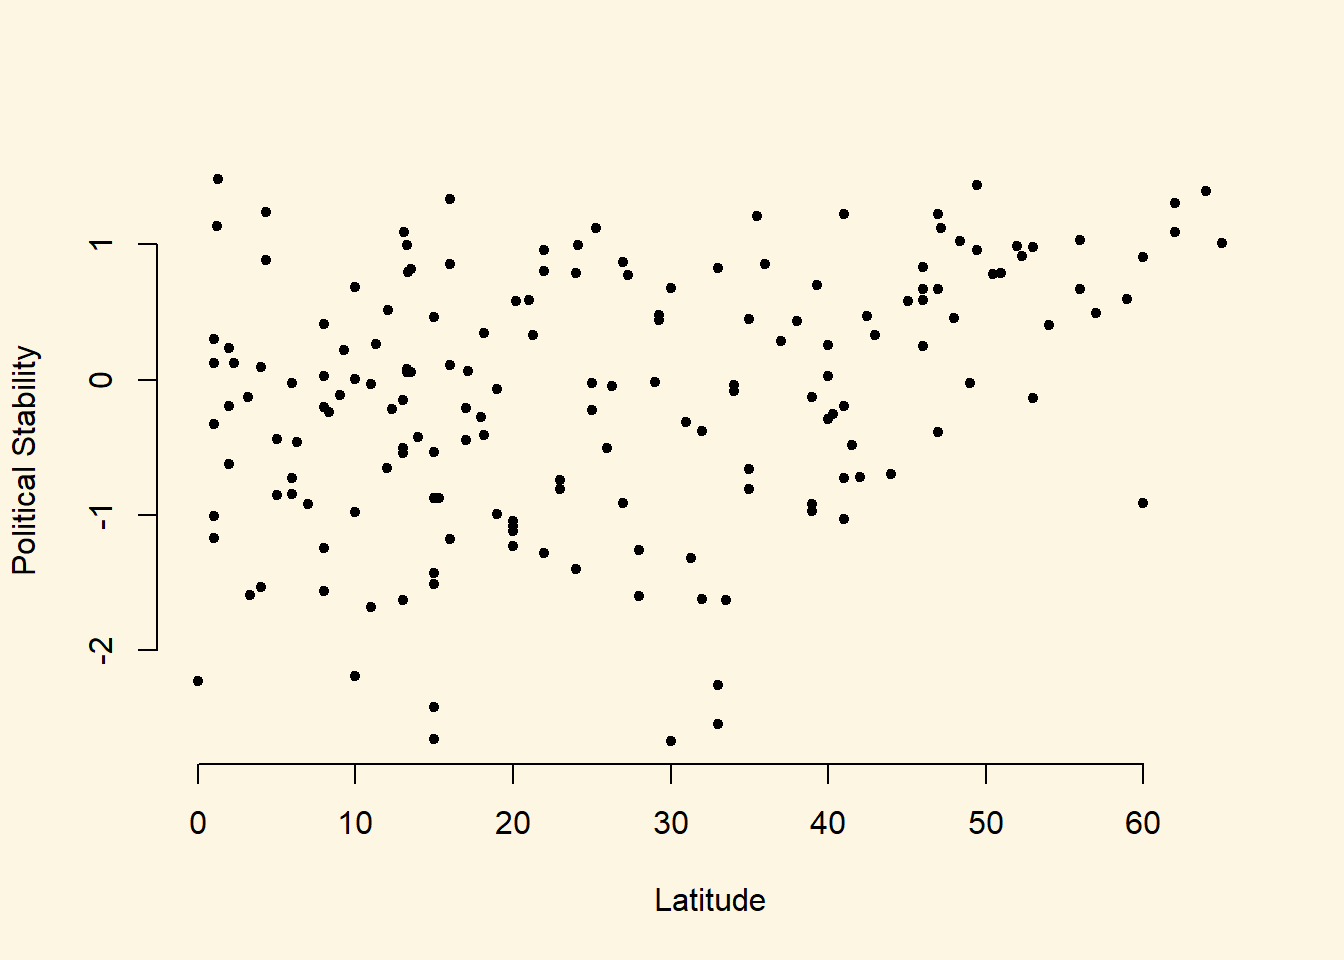
\includegraphics{suffolk2019_files/figure-latex/unnamed-chunk-151-1.pdf}

Looking at the cloud of points suggests that there might be a positive relationship: increases in our independent variable \texttt{latitude} appear to be associated with increases in the dependent variable \texttt{pol\_stability} (the further from the equator, the more stable).

We can fit a line of best fit through the points. To do this we must estimate the bivariate regression model with the \texttt{lm()} function.

\begin{Shaded}
\begin{Highlighting}[]
\NormalTok{latitude_model <-}\StringTok{ }\KeywordTok{lm}\NormalTok{(pol_stability }\OperatorTok{~}\StringTok{ }\NormalTok{latitude, }\DataTypeTok{data =}\NormalTok{ world_data)}
\end{Highlighting}
\end{Shaded}

Now we can create a scatterplot with a regression line using the \texttt{abline()} function.

\begin{Shaded}
\begin{Highlighting}[]
\KeywordTok{plot}\NormalTok{(}\DataTypeTok{x =}\NormalTok{ world_data}\OperatorTok{$}\NormalTok{latitude,}
     \DataTypeTok{y =}\NormalTok{ world_data}\OperatorTok{$}\NormalTok{pol_stability,}
     \DataTypeTok{frame.plot =} \OtherTok{FALSE}\NormalTok{,}
     \DataTypeTok{pch =} \DecValTok{20}\NormalTok{,}
     \DataTypeTok{xlab =} \StringTok{"Latitude"}\NormalTok{,}
     \DataTypeTok{ylab =} \StringTok{"Political Stability"}\NormalTok{)}

\KeywordTok{abline}\NormalTok{(latitude_model, }\DataTypeTok{col =} \StringTok{"red"}\NormalTok{)}
\end{Highlighting}
\end{Shaded}

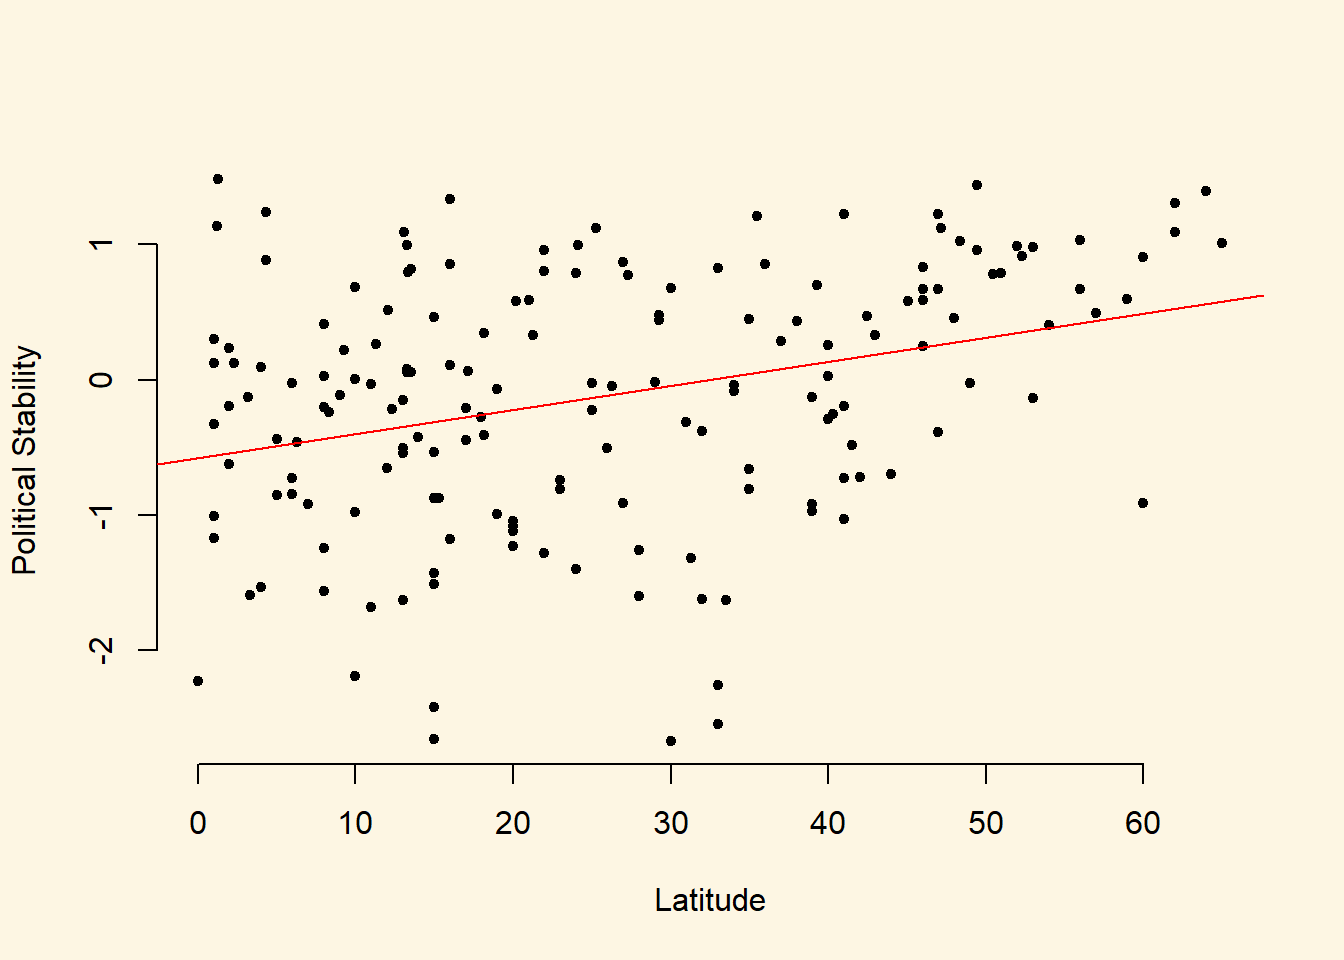
\includegraphics{suffolk2019_files/figure-latex/unnamed-chunk-153-1.pdf}

We can also view a simple summary of the regression by using the \texttt{screenreg} function:

\begin{Shaded}
\begin{Highlighting}[]
\KeywordTok{screenreg}\NormalTok{(latitude_model)}
\end{Highlighting}
\end{Shaded}

\begin{verbatim}

=======================
             Model 1   
-----------------------
(Intercept)   -0.58 ***
              (0.12)   
latitude       0.02 ***
              (0.00)   
-----------------------
R^2            0.11    
Adj. R^2       0.10    
Num. obs.    170       
RMSE           0.89    
=======================
*** p < 0.001, ** p < 0.01, * p < 0.05
\end{verbatim}

Thinking back to earlier today, how do we interpret this regression?

\begin{itemize}
\tightlist
\item
  The coefficient for the variable \texttt{latitude} (\(\beta_1\)) indicates that a one-unit increase in a country's latitude is associated with a 0.0178378 increase in the measure of political stability, on average. Question: Is this association statistically significant at the 95\% confidence level?
\item
  The coefficient for the \texttt{(intercept)} term (\(\beta_0\)) indicates that the average level of political stability for a country with a latitude of 0 is -0.580075 (where \texttt{latitude\ =\ 0} is a country positioned at the equator)
\item
  The \(R^2\) of the model is 0.1065267. This implies that 11\% of the variation in the dependent variable (political stability) is explained by the independent variable (latitude) in the model.
\end{itemize}

The regression above suggests that there is a significant association between these variables However, as good social scientistis, we probably do not think that the distance of a country from the equator is a theoretically relevant variable for explaining political stability. This is because there is no plausible causal link between the two. We should therefore consider other variables to include in our model.

We will include the index of globalization (higher values mean more integration with the rest of the world), the quality of institutions, and the indicator for whether the country is a democracy. For all of these variables we can come up with a theoretical story for their effect on political stability.

To specify a \emph{multiple} linear regression model, the only thing we need to change is the \texttt{formula} argument of the \texttt{lm()} function. In particular, if we wish to add additional explanatory variables, the formula argument will take the following form:

\begin{Shaded}
\begin{Highlighting}[]
\NormalTok{dependent.var }\OperatorTok{~}\StringTok{ }\NormalTok{independent.var}\FloatTok{.1} \OperatorTok{+}\StringTok{ }\NormalTok{independent.var}\FloatTok{.2} \OperatorTok{+}\StringTok{ }\NormalTok{independent.var}\FloatTok{.3}\NormalTok{ ...}
\end{Highlighting}
\end{Shaded}

In our example here, the model would therefore look like the following:

\begin{Shaded}
\begin{Highlighting}[]
\NormalTok{inst_model <-}\StringTok{ }\KeywordTok{lm}\NormalTok{(}
\NormalTok{  pol_stability }\OperatorTok{~}\StringTok{ }\NormalTok{latitude }\OperatorTok{+}\StringTok{ }\NormalTok{globalization }\OperatorTok{+}\StringTok{ }\NormalTok{inst_quality }\OperatorTok{+}\StringTok{ }\NormalTok{democracy, }
  \DataTypeTok{data =}\NormalTok{ world_data}
\NormalTok{)}
\end{Highlighting}
\end{Shaded}

Remember, \texttt{pol\_stability} is our dependent variable, as before, and now we have four independent variables: \texttt{latitude}, \texttt{globalization}, \texttt{democracy} and \texttt{inst\_quality}. Again, just as with the bivariate model, we can view the summarised output of the regression by using \texttt{screenreg()}. As we now have two models (a simple regression model, and a multiple regression model), we can join them together using the \texttt{list()} function, and then put all of that inside \texttt{screenreg()}.

\begin{Shaded}
\begin{Highlighting}[]
\KeywordTok{screenreg}\NormalTok{(}\KeywordTok{list}\NormalTok{(latitude_model, inst_model))}
\end{Highlighting}
\end{Shaded}

\begin{verbatim}

=============================================
                       Model 1     Model 2   
---------------------------------------------
(Intercept)             -0.58 ***   -1.25 ***
                        (0.12)      (0.20)   
latitude                 0.02 ***    0.00    
                        (0.00)      (0.00)   
globalization                       -0.00    
                                    (0.01)   
inst_quality                         0.34 ***
                                    (0.04)   
democracy1. Democracy                0.04    
                                    (0.11)   
---------------------------------------------
R^2                      0.11        0.50    
Adj. R^2                 0.10        0.49    
Num. obs.              170         170       
RMSE                     0.89        0.67    
=============================================
*** p < 0.001, ** p < 0.01, * p < 0.05
\end{verbatim}

Including the two new predictors leads to substantial changes.

\begin{itemize}
\tightlist
\item
  First, we now explain 50\% of the variance of our dependent variable instead of just 11\%.
\item
  Second, the effect of the distance to the equator is no longer significant.
\item
  Third, better quality institutions are associated with more political stability. In particular, a one-unit increase in the measure of instituion quality (which ranges from 1 to 10) is associated with a 0.338882 increase in the measure for political stability.
\item
  Fourth, there is no significant relationship between globalization and political stability in this data.
\item
  Fifth, there is no significant relationship between democracy and political stability in this data.
\end{itemize}

\#\#\# Predicting outcome conditional on institutional quality

Just as we did with the simple regression model last week, we can use the fitted model object to calculate the fitted values of our dependent variable for different values of our explanatory variables. To do so, we again use the \texttt{predict()} function.

We proceed in three steps.

\begin{enumerate}
\def\labelenumi{\arabic{enumi}.}
\tightlist
\item
  We set the values of the covariates for which we would like to produce fitted values.

  \begin{itemize}
  \tightlist
  \item
    You will need to set covariate values for \emph{every} explanatory variable that you included in your model.
  \item
    As only one of our variables has a significant relationship with the outcome in the multiple regression model that we estimated above, we are really only interested in that variable (\texttt{inst\_quality}).
  \item
    Therefore, we will calculate fitted values over the range of \texttt{inst\_quality}, while setting the values of \texttt{latitude} and \texttt{globalization} to their mean values.
  \item
    As \texttt{democracy} is a factor variable, we cannot use the mean value. Instead, we will set \texttt{democracy} to be equal to \texttt{"1.\ Democracy"} which is the label for democratic countries
  \end{itemize}
\item
  We calculate the fitted values.
\item
  We report the results (here we will produce a plot).
\end{enumerate}

For step one, the following code produces a \texttt{data.frame} of new covariate values for which we would like to calculate a fitted value from our model:

\begin{Shaded}
\begin{Highlighting}[]
\NormalTok{democracies <-}\StringTok{ }\KeywordTok{data.frame}\NormalTok{(}
  \DataTypeTok{inst_quality =} \KeywordTok{seq}\NormalTok{(}\DataTypeTok{from =} \FloatTok{1.4}\NormalTok{, }\DataTypeTok{to =} \FloatTok{9.3}\NormalTok{, }\DataTypeTok{by =} \DecValTok{1}\NormalTok{),}
  \DataTypeTok{globalization =} \KeywordTok{mean}\NormalTok{(world_data}\OperatorTok{$}\NormalTok{globalization),}
  \DataTypeTok{latitude =} \KeywordTok{mean}\NormalTok{(world_data}\OperatorTok{$}\NormalTok{latitude),}
  \DataTypeTok{democracy =} \StringTok{"1. Democracy"}
\NormalTok{)}
\end{Highlighting}
\end{Shaded}

We've just created a \texttt{data.frame} of hypothetical democracies with varying level of institutional quality. Let's see what this \texttt{data.frame} looks like.

\begin{Shaded}
\begin{Highlighting}[]
\NormalTok{democracies}
\end{Highlighting}
\end{Shaded}

\begin{verbatim}
  inst_quality globalization latitude    democracy
1          1.4      57.93053 25.78218 1. Democracy
2          2.4      57.93053 25.78218 1. Democracy
3          3.4      57.93053 25.78218 1. Democracy
4          4.4      57.93053 25.78218 1. Democracy
5          5.4      57.93053 25.78218 1. Democracy
6          6.4      57.93053 25.78218 1. Democracy
7          7.4      57.93053 25.78218 1. Democracy
8          8.4      57.93053 25.78218 1. Democracy
\end{verbatim}

In this \texttt{data.frame}, we have set the \texttt{inst\_quality} variable to vary between 1.4 and 9.3000002, with increments of 1 unit which represents the range of \texttt{inst\_quality} in our dataset.

\begin{Shaded}
\begin{Highlighting}[]
\KeywordTok{min}\NormalTok{(world_data}\OperatorTok{$}\NormalTok{inst_quality)}
\end{Highlighting}
\end{Shaded}

\begin{verbatim}
[1] 1.4
\end{verbatim}

\begin{Shaded}
\begin{Highlighting}[]
\KeywordTok{max}\NormalTok{(world_data}\OperatorTok{$}\NormalTok{inst_quality)}
\end{Highlighting}
\end{Shaded}

\begin{verbatim}
[1] 9.3
\end{verbatim}

We have set \texttt{globalization} to be equal to the mean value of \texttt{globalization} in the \texttt{world\_data} object, and \texttt{latitude} to be equal to the mean value of \texttt{latitude} in the \texttt{world\_data} object. Finally, we have set \texttt{democracy} to be equal to \texttt{"1.\ Democracy"} (the value for democratic countries).

We can now calculate the fitted values for each of these combinations of our explanatory variables using the \texttt{predict()} function.

\begin{Shaded}
\begin{Highlighting}[]
\NormalTok{democracies}\OperatorTok{$}\NormalTok{predicted_pol_stability <-}\StringTok{ }\KeywordTok{predict}\NormalTok{(inst_model, }\DataTypeTok{newdata =}\NormalTok{ democracies)}
\end{Highlighting}
\end{Shaded}

We can now look again at the \texttt{democracies} object:

\begin{Shaded}
\begin{Highlighting}[]
\NormalTok{democracies}
\end{Highlighting}
\end{Shaded}

\begin{verbatim}
  inst_quality globalization latitude    democracy predicted_pol_stability
1          1.4      57.93053 25.78218 1. Democracy             -1.00319887
2          2.4      57.93053 25.78218 1. Democracy             -0.66431685
3          3.4      57.93053 25.78218 1. Democracy             -0.32543483
4          4.4      57.93053 25.78218 1. Democracy              0.01344719
5          5.4      57.93053 25.78218 1. Democracy              0.35232921
6          6.4      57.93053 25.78218 1. Democracy              0.69121123
7          7.4      57.93053 25.78218 1. Democracy              1.03009325
8          8.4      57.93053 25.78218 1. Democracy              1.36897527
\end{verbatim}

Hey presto! Now, for each of our explanatory variable combinations, we have the corresponding fitted values as calculated from our estimated regression.

Finally, we can plot these values:

\begin{Shaded}
\begin{Highlighting}[]
\KeywordTok{plot}\NormalTok{(}
  \DataTypeTok{x =}\NormalTok{ democracies}\OperatorTok{$}\NormalTok{inst_quality,}
  \DataTypeTok{y =}\NormalTok{ democracies}\OperatorTok{$}\NormalTok{predicted_pol_stability,}
  \DataTypeTok{frame.plot =} \OtherTok{FALSE}\NormalTok{, }
  \DataTypeTok{col =} \StringTok{"blue"}\NormalTok{,}
  \DataTypeTok{type =} \StringTok{"l"}\NormalTok{,}
  \DataTypeTok{xlab =} \StringTok{"Institution Quality"}\NormalTok{, }
  \DataTypeTok{ylab =} \StringTok{"Fitted value for political stability"}
\NormalTok{)}
\end{Highlighting}
\end{Shaded}

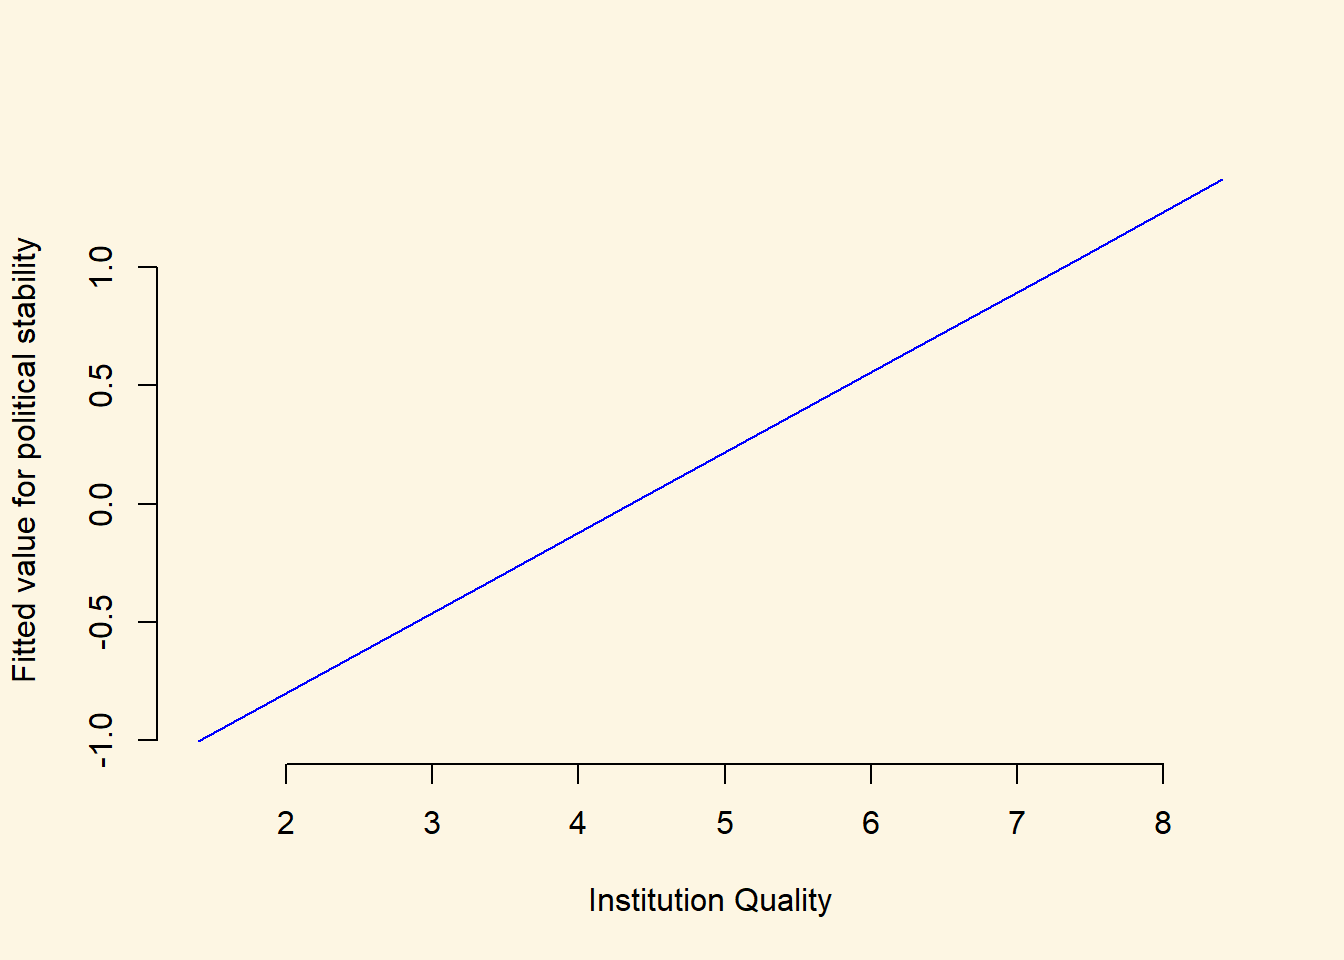
\includegraphics{suffolk2019_files/figure-latex/unnamed-chunk-165-1.pdf}

We could also use the output from our model to plot two separate lines of fitted values: one for democracies, and one for dictatorships. We have already done this for democracies, so the following code constructs a \texttt{data.frame} of fitted values for dictatorships:

\begin{Shaded}
\begin{Highlighting}[]
\NormalTok{dictatorships <-}\StringTok{ }\KeywordTok{data.frame}\NormalTok{(}
  \DataTypeTok{inst_quality =} \KeywordTok{seq}\NormalTok{(}\DataTypeTok{from =} \FloatTok{1.4}\NormalTok{, }\DataTypeTok{to =} \FloatTok{9.3}\NormalTok{, }\DataTypeTok{by =} \DecValTok{1}\NormalTok{),}
  \DataTypeTok{globalization =} \KeywordTok{mean}\NormalTok{(world_data}\OperatorTok{$}\NormalTok{globalization),}
  \DataTypeTok{latitude =} \KeywordTok{mean}\NormalTok{(world_data}\OperatorTok{$}\NormalTok{latitude),}
  \DataTypeTok{democracy =} \StringTok{"0. Dictatorship"}
\NormalTok{)}

\NormalTok{dictatorships}\OperatorTok{$}\NormalTok{predicted_pol_stability <-}\StringTok{ }\KeywordTok{predict}\NormalTok{(inst_model, }\DataTypeTok{newdata =}\NormalTok{ dictatorships)}
\end{Highlighting}
\end{Shaded}

Now that we have calculated these fitted values, we can add the line for dictatorships to the plot we created above using the \texttt{lines()} function:

\begin{Shaded}
\begin{Highlighting}[]
\KeywordTok{plot}\NormalTok{(}
  \DataTypeTok{x =}\NormalTok{ democracies}\OperatorTok{$}\NormalTok{inst_quality,}
  \DataTypeTok{y =}\NormalTok{ democracies}\OperatorTok{$}\NormalTok{predicted_pol_stability,}
  \DataTypeTok{frame.plot =} \OtherTok{FALSE}\NormalTok{, }
  \DataTypeTok{col =} \StringTok{"blue"}\NormalTok{,}
  \DataTypeTok{type =} \StringTok{"l"}\NormalTok{,}
  \DataTypeTok{xlab =} \StringTok{"Institution Quality"}\NormalTok{, }
  \DataTypeTok{ylab =} \StringTok{"Fitted value for political stability"}
\NormalTok{)}

\KeywordTok{lines}\NormalTok{(}\DataTypeTok{x =}\NormalTok{ dictatorships}\OperatorTok{$}\NormalTok{inst_quality,}
      \DataTypeTok{y =}\NormalTok{ dictatorships}\OperatorTok{$}\NormalTok{predicted_pol_stability,}
      \DataTypeTok{data =}\NormalTok{ dictatorships,}
      \DataTypeTok{col =} \StringTok{"red"}\NormalTok{)}
\end{Highlighting}
\end{Shaded}

\begin{verbatim}
Warning in plot.xy(xy.coords(x, y), type = type, ...): "data" is not a
graphical parameter
\end{verbatim}

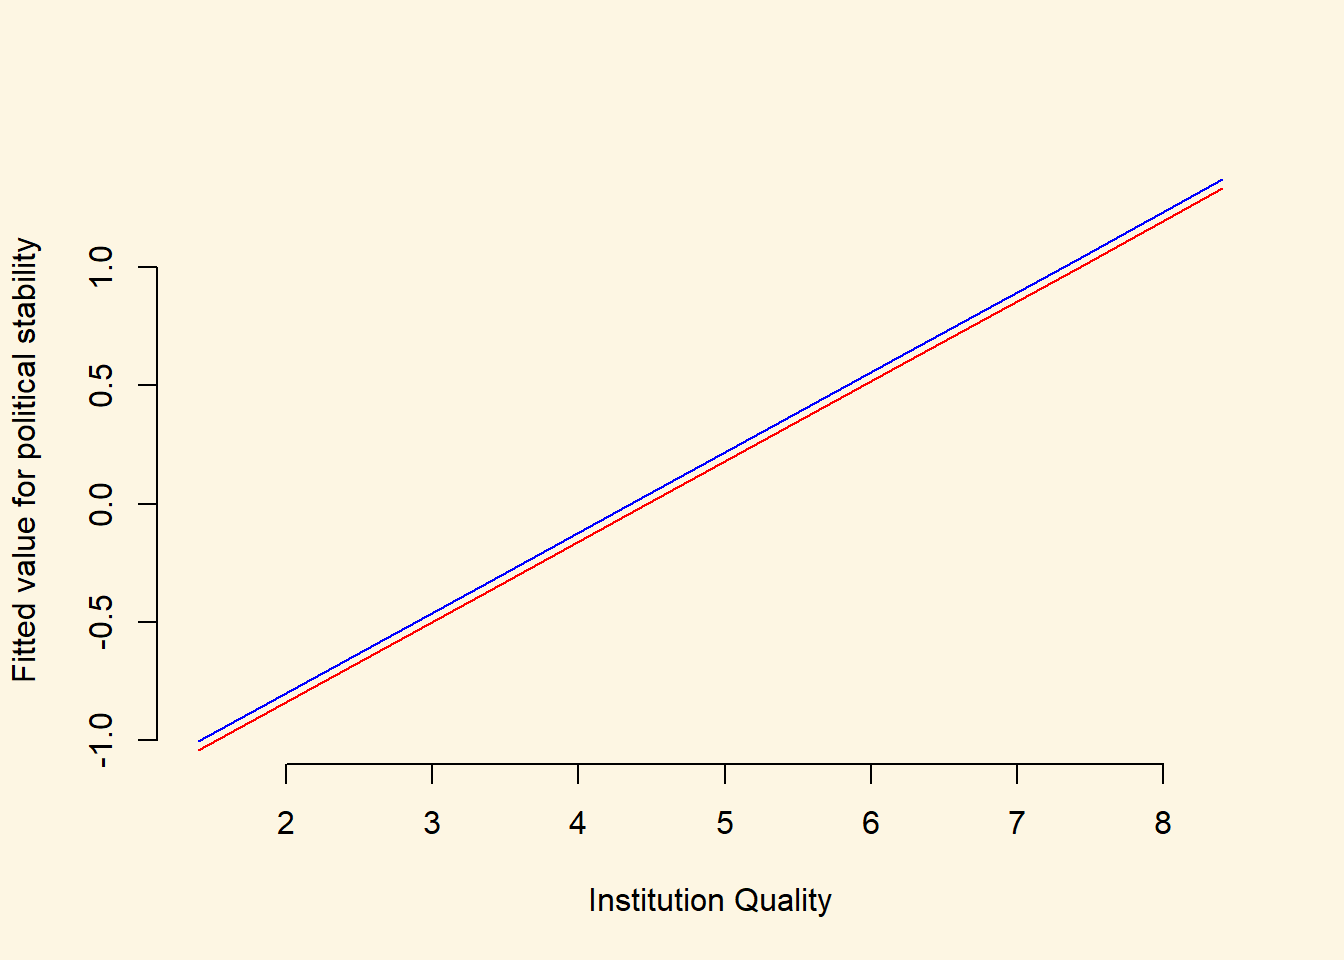
\includegraphics{suffolk2019_files/figure-latex/unnamed-chunk-167-1.pdf}

We can see from the plot that the fitted values for democracies (blue line) are almost exactly the same as those for dictatorships (red line). This is reassuring, as the estimated coefficient on the democracy variable was very small (0.04) and was not statistically significantly different from 0. Often, however, it can be very illuminating to construct plots like this where we construct a line to indicate how our predicted values for Y vary across one of our explanatory variables (here, institution quality), and we create different lines for different values of another explanatory variable (here, democracy/dictatorship).

\hypertarget{non-linearities}{%
\subsubsection{Non-Linearities}\label{non-linearities}}

Let's clear our workspace for now to keep the workspace tidy and to prevent our computer from slowing down.

\begin{Shaded}
\begin{Highlighting}[]
\KeywordTok{rm}\NormalTok{(}\DataTypeTok{list =} \KeywordTok{ls}\NormalTok{())}
\end{Highlighting}
\end{Shaded}

We will use the small version of the Quality of Government data from 2012 again (\texttt{QoG2012.csv}) with four variables:

\begin{longtable}[]{@{}ll@{}}
\toprule
\begin{minipage}[b]{0.17\columnwidth}\raggedright
Variable\strut
\end{minipage} & \begin{minipage}[b]{0.77\columnwidth}\raggedright
Description\strut
\end{minipage}\tabularnewline
\midrule
\endhead
\begin{minipage}[t]{0.17\columnwidth}\raggedright
\texttt{former\_col}\strut
\end{minipage} & \begin{minipage}[t]{0.77\columnwidth}\raggedright
0 = not a former colony 1 = former colony\strut
\end{minipage}\tabularnewline
\begin{minipage}[t]{0.17\columnwidth}\raggedright
\texttt{undp\_hdi}\strut
\end{minipage} & \begin{minipage}[t]{0.77\columnwidth}\raggedright
UNDP Human Development Index. Higher values mean better quality of life\strut
\end{minipage}\tabularnewline
\begin{minipage}[t]{0.17\columnwidth}\raggedright
\texttt{wbgi\_cce}\strut
\end{minipage} & \begin{minipage}[t]{0.77\columnwidth}\raggedright
Control of corruption. Higher values mean better control of corruption\strut
\end{minipage}\tabularnewline
\begin{minipage}[t]{0.17\columnwidth}\raggedright
\texttt{wdi\_gdpc}\strut
\end{minipage} & \begin{minipage}[t]{0.77\columnwidth}\raggedright
GDP per capita in US dollars\strut
\end{minipage}\tabularnewline
\bottomrule
\end{longtable}

\begin{Shaded}
\begin{Highlighting}[]
\NormalTok{world_data <-}\StringTok{ }\KeywordTok{read.csv}\NormalTok{(}\StringTok{"QoG2012.csv"}\NormalTok{)}
\KeywordTok{names}\NormalTok{(world_data)}
\end{Highlighting}
\end{Shaded}

\begin{verbatim}
[1] "h_j"         "wdi_gdpc"    "undp_hdi"    "wbgi_cce"    "wbgi_pse"   
[6] "former_col"  "lp_lat_abst"
\end{verbatim}

Rename the variables by yourself to:

\begin{longtable}[]{@{}ll@{}}
\toprule
New Name & Old Name\tabularnewline
\midrule
\endhead
\texttt{human\_development} & \texttt{undp\_hdi}\tabularnewline
\texttt{institutions\_quality} & \texttt{wbgi\_cce}\tabularnewline
\texttt{gdp\_capita} & \texttt{wdi\_gdpc}\tabularnewline
\bottomrule
\end{longtable}

\begin{Shaded}
\begin{Highlighting}[]
\KeywordTok{names}\NormalTok{(world_data)}
\end{Highlighting}
\end{Shaded}

\begin{verbatim}
[1] "h_j"         "wdi_gdpc"    "undp_hdi"    "wbgi_cce"    "wbgi_pse"   
[6] "former_col"  "lp_lat_abst"
\end{verbatim}

\begin{Shaded}
\begin{Highlighting}[]
\KeywordTok{names}\NormalTok{(world_data)[}\KeywordTok{names}\NormalTok{(world_data)}\OperatorTok{==}\StringTok{"undp_hdi"}\NormalTok{] <-}\StringTok{ "human_development"}
\KeywordTok{names}\NormalTok{(world_data)[}\KeywordTok{names}\NormalTok{(world_data)}\OperatorTok{==}\StringTok{"wbgi_cce"}\NormalTok{] <-}\StringTok{ "institutions_quality"}
\KeywordTok{names}\NormalTok{(world_data)[}\KeywordTok{names}\NormalTok{(world_data)}\OperatorTok{==}\StringTok{"wdi_gdpc"}\NormalTok{] <-}\StringTok{ "gdp_capita"}
\KeywordTok{names}\NormalTok{(world_data)}
\end{Highlighting}
\end{Shaded}

\begin{verbatim}
[1] "h_j"                  "gdp_capita"           "human_development"   
[4] "institutions_quality" "wbgi_pse"             "former_col"          
[7] "lp_lat_abst"         
\end{verbatim}

Now let's look at the summary statistics for the entire data set.

\begin{Shaded}
\begin{Highlighting}[]
\KeywordTok{summary}\NormalTok{(world_data) }
\end{Highlighting}
\end{Shaded}

\begin{verbatim}
      h_j           gdp_capita      human_development institutions_quality
 Min.   :0.0000   Min.   :  226.2   Min.   :0.2730    Min.   :-1.69953    
 1st Qu.:0.0000   1st Qu.: 1768.0   1st Qu.:0.5390    1st Qu.:-0.81965    
 Median :0.0000   Median : 5326.1   Median :0.7510    Median :-0.30476    
 Mean   :0.3787   Mean   :10184.1   Mean   :0.6982    Mean   :-0.05072    
 3rd Qu.:1.0000   3rd Qu.:12976.5   3rd Qu.:0.8335    3rd Qu.: 0.50649    
 Max.   :1.0000   Max.   :63686.7   Max.   :0.9560    Max.   : 2.44565    
 NA's   :25       NA's   :16        NA's   :19        NA's   :2           
    wbgi_pse          former_col      lp_lat_abst    
 Min.   :-2.46746   Min.   :0.0000   Min.   :0.0000  
 1st Qu.:-0.72900   1st Qu.:0.0000   1st Qu.:0.1343  
 Median : 0.02772   Median :1.0000   Median :0.2444  
 Mean   :-0.03957   Mean   :0.6289   Mean   :0.2829  
 3rd Qu.: 0.79847   3rd Qu.:1.0000   3rd Qu.:0.4444  
 Max.   : 1.67561   Max.   :1.0000   Max.   :0.7222  
                                     NA's   :7       
\end{verbatim}

We need to remove missing values from \texttt{gdp\_capita}, \texttt{human\_development}, and \texttt{institutions\_quality}. Do so yourself. Do not drop observations that missing values on other observations such as \texttt{lp\_lat\_abst}. We might throw away useful information when doing so.

\begin{Shaded}
\begin{Highlighting}[]
\NormalTok{world_data <-}\StringTok{ }\NormalTok{world_data[ }\OperatorTok{!}\KeywordTok{is.na}\NormalTok{(world_data}\OperatorTok{$}\NormalTok{gdp_capita), ]}
\NormalTok{world_data <-}\StringTok{ }\NormalTok{world_data[ }\OperatorTok{!}\KeywordTok{is.na}\NormalTok{(world_data}\OperatorTok{$}\NormalTok{human_development), ]}
\NormalTok{world_data <-}\StringTok{ }\NormalTok{world_data[ }\OperatorTok{!}\KeywordTok{is.na}\NormalTok{(world_data}\OperatorTok{$}\NormalTok{institutions_quality), ]}
\end{Highlighting}
\end{Shaded}

Let's suppose we want to illustrate the relationship between GDP per capita and the human development index. We draw a scatter plot to investigate the relationship between the quality of life (hdi) and wealth (gdp/captia).

\begin{Shaded}
\begin{Highlighting}[]
\KeywordTok{plot}\NormalTok{(}
  \DataTypeTok{x =}\NormalTok{ world_data}\OperatorTok{$}\NormalTok{gdp_capita,}
  \DataTypeTok{y =}\NormalTok{ world_data}\OperatorTok{$}\NormalTok{human_development,}
  \DataTypeTok{data =}\NormalTok{ world_data,}
  \DataTypeTok{pch =} \DecValTok{20}\NormalTok{,}
  \DataTypeTok{frame.plot =} \OtherTok{FALSE}\NormalTok{,}
  \DataTypeTok{col =} \StringTok{"grey"}\NormalTok{,}
  \DataTypeTok{main =} \StringTok{"Relationship between the quality of life and wealth"}\NormalTok{,}
  \DataTypeTok{ylab =} \StringTok{"Human development index"}\NormalTok{,}
  \DataTypeTok{xlab =} \StringTok{"GDP per capita"}
\NormalTok{)}
\end{Highlighting}
\end{Shaded}

\begin{verbatim}
Warning in plot.window(...): "data" is not a graphical parameter
\end{verbatim}

\begin{verbatim}
Warning in plot.xy(xy, type, ...): "data" is not a graphical parameter
\end{verbatim}

\begin{verbatim}
Warning in axis(side = side, at = at, labels = labels, ...): "data" is not
a graphical parameter

Warning in axis(side = side, at = at, labels = labels, ...): "data" is not
a graphical parameter
\end{verbatim}

\begin{verbatim}
Warning in title(...): "data" is not a graphical parameter
\end{verbatim}

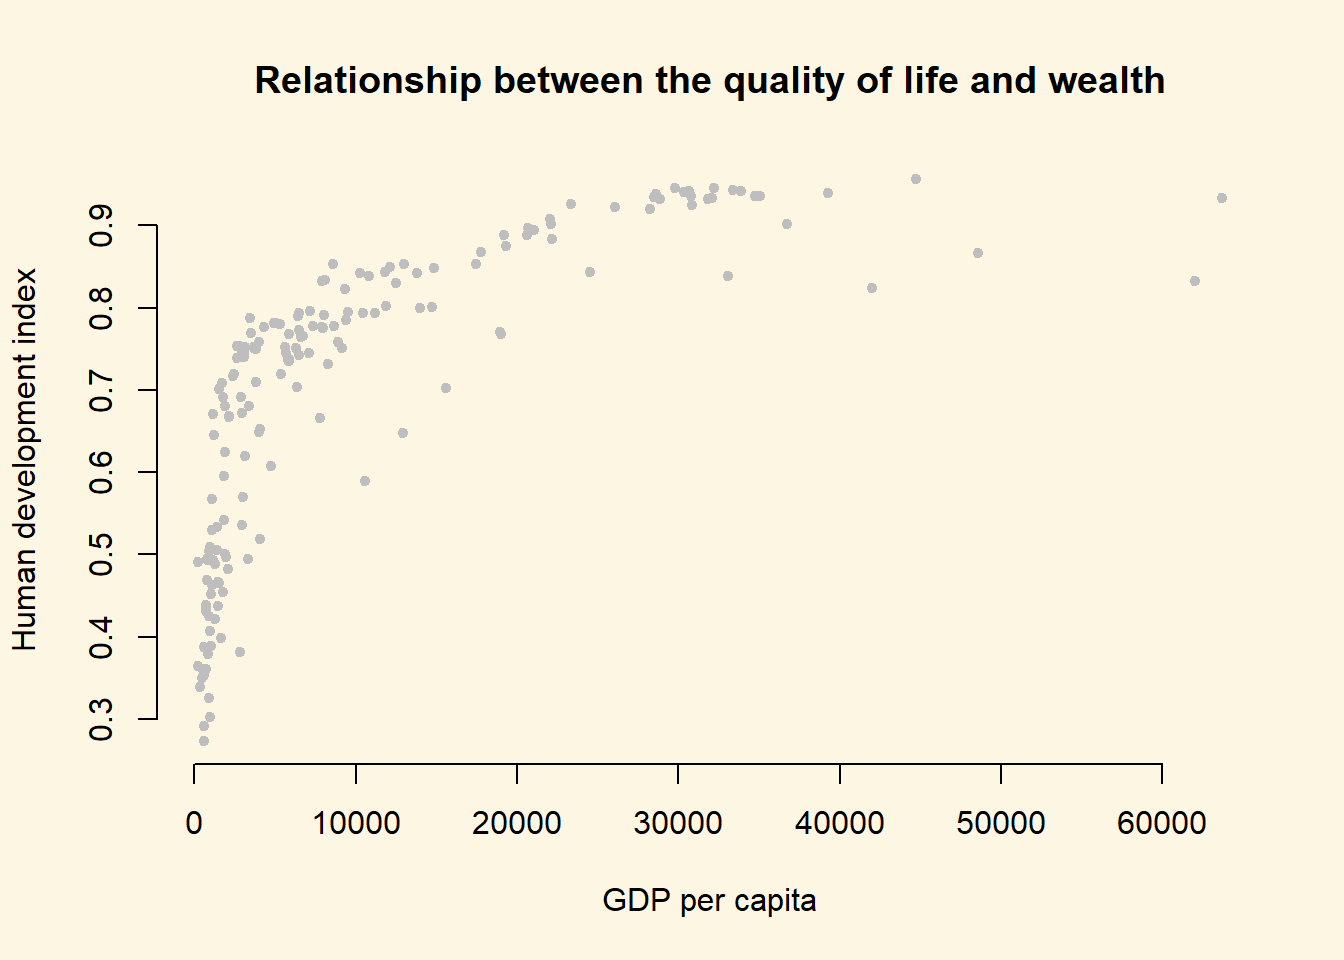
\includegraphics{suffolk2019_files/figure-latex/unnamed-chunk-173-1.pdf}

It's easy to see, that the relationship between GDP per captia and the Human Development Index is not linear. Increases in wealth rapidly increase the quality of life in poor societies. The richer the country, the less pronounced the effect of additional wealth. We would mis-specify our model if we do not take the non-linear relationship into account.

Let's go ahead and fit a mis-specified model:

\begin{Shaded}
\begin{Highlighting}[]
\NormalTok{linear.model <-}\StringTok{ }\KeywordTok{lm}\NormalTok{(human_development }\OperatorTok{~}\StringTok{ }\NormalTok{gdp_capita, }\DataTypeTok{data =}\NormalTok{ world_data)}
\KeywordTok{screenreg}\NormalTok{(linear.model)}
\end{Highlighting}
\end{Shaded}

\begin{verbatim}

=======================
             Model 1   
-----------------------
(Intercept)    0.59 ***
              (0.01)   
gdp_capita     0.00 ***
              (0.00)   
-----------------------
R^2            0.49    
Adj. R^2       0.49    
Num. obs.    172       
RMSE           0.13    
=======================
*** p < 0.001, ** p < 0.01, * p < 0.05
\end{verbatim}

We detect a significant linear relationship. The effect may look small because the coefficient rounded to two digits is zero. But remember, this is the effect of increasing GDP/capita by \(1\) US dollar on the quality of life. That effect is naturally small but it is probably not small when we increase wealth by \(1000\) US dollars.

However, our model would also entail that for every increase in GDP/capita, the quality of life increases on average by the same amount. We saw from our plot that this is not the case. The effect of GDP/capita on the quality of life is conditional on the level of GDP/capita. If that sounds like an interaction to you, then that is great because, we will model the non-linearity by raising the GDP/capita to a higher power. That is in effect an interaction of the variable with itself. GDP/capita raised to the second power, e.g.~is GDP/capita * GDP/capita.

\hypertarget{polynomials}{%
\paragraph{Polynomials}\label{polynomials}}

We know from school that polynomials like \(X^2\), \(X^3\) and so on are not linear. The relationship depicted in our plot above suggests a quadratic relationship between GDP per capita and the human development index might be appropriate (there is only one obvious ``bend'' in the data). To incorporate this intuition into our model, we will use the \texttt{poly()} function in our linear model to raise GDP/capita to the second power like so: \texttt{poly(gdp\_capita,\ degree\ =\ 2).}

\begin{Shaded}
\begin{Highlighting}[]
\NormalTok{quadratic.model <-}\StringTok{ }\KeywordTok{lm}\NormalTok{(}
\NormalTok{  human_development }\OperatorTok{~}\StringTok{ }\KeywordTok{poly}\NormalTok{(gdp_capita, }\DataTypeTok{degree =} \DecValTok{2}\NormalTok{), }
  \DataTypeTok{data =}\NormalTok{ world_data}
\NormalTok{)}


\KeywordTok{screenreg}\NormalTok{(}
  \KeywordTok{list}\NormalTok{(linear.model, quadratic.model), }
  \DataTypeTok{custom.model.names =} \KeywordTok{c}\NormalTok{(}\StringTok{"Linear model"}\NormalTok{, }\StringTok{"Quadratic model"}\NormalTok{)}
\NormalTok{)}
\end{Highlighting}
\end{Shaded}

\begin{verbatim}

============================================================
                               Linear model  Quadratic model
------------------------------------------------------------
(Intercept)                      0.59 ***      0.70 ***     
                                (0.01)        (0.01)        
gdp_capita                       0.00 ***                   
                                (0.00)                      
poly(gdp_capita, degree = 2)1                  1.66 ***     
                                              (0.10)        
poly(gdp_capita, degree = 2)2                 -1.00 ***     
                                              (0.10)        
------------------------------------------------------------
R^2                              0.49          0.67         
Adj. R^2                         0.49          0.66         
Num. obs.                      172           172            
RMSE                             0.13          0.10         
============================================================
*** p < 0.001, ** p < 0.01, * p < 0.05
\end{verbatim}

It is important to note, that in the quadratic model the effect of GDP/capita is no longer easy to interpret. We cannot say for every increase in GDP/capita by one dollar, the quality of life increases on average by some fixed amount. This is because the effect of GDP/capita depends on how rich a country was to begin with. We can, however, interpret the statitical significance of the quadratic term: the coefficient is about 10 times as large in absolute terms as the standard error, meaning we can easily reject the null hypothesis that the relationship between GDP and the HDI is linear. Furthermore, it looks like our model that includes the quadratic term has a much better fit, as the adjusted \(R^2\) has increased by a lot.

We can interpret the effect of wealth (GDP/capita) on the quality of life (human development index) by predicting the fitted values of the human development index given a certain level of GDP/capita. We will vary GDP/captia from its minimum in the data to its maximum and the plot the results which is a good way to illustrate a non-linear relationship.

Step 1: We find the minimum and maximum values of GDP/capita.

\begin{Shaded}
\begin{Highlighting}[]
\KeywordTok{range}\NormalTok{(world_data}\OperatorTok{$}\NormalTok{gdp_capita)}
\end{Highlighting}
\end{Shaded}

\begin{verbatim}
[1]   226.235 63686.676
\end{verbatim}

Step 2: We predict fitted values for varying levels of GDP/captia (let's create 100 predictions).

We create our sequence of 100 GDP/capita values

\begin{Shaded}
\begin{Highlighting}[]
\NormalTok{gdp_seq <-}\StringTok{ }\KeywordTok{seq}\NormalTok{(}\DataTypeTok{from =} \DecValTok{226}\NormalTok{, }\DataTypeTok{to =} \DecValTok{63686}\NormalTok{, }\DataTypeTok{length.out =} \DecValTok{100}\NormalTok{)}
\end{Highlighting}
\end{Shaded}

We set our covariate values (here we only have one covariate: GDP/captia)

\begin{Shaded}
\begin{Highlighting}[]
\NormalTok{x <-}\StringTok{ }\KeywordTok{data.frame}\NormalTok{(}\DataTypeTok{gdp_capita =}\NormalTok{ gdp_seq)}
\end{Highlighting}
\end{Shaded}

We predict the outcome (human development index) for each of the 100 GDP levels

\begin{Shaded}
\begin{Highlighting}[]
\NormalTok{y_hat <-}\StringTok{ }\KeywordTok{predict}\NormalTok{(quadratic.model, }\DataTypeTok{newdata =}\NormalTok{ x)}
\end{Highlighting}
\end{Shaded}

Step 3: Now that we have created our predictions. We plot again and then we add the \texttt{linear.model} using \texttt{abline} and we add our non-linear version \texttt{quadratic.model} using the \texttt{lines()} function.

\begin{Shaded}
\begin{Highlighting}[]
\KeywordTok{plot}\NormalTok{(}
  \DataTypeTok{x =}\NormalTok{ world_data}\OperatorTok{$}\NormalTok{gdp_capita,}
  \DataTypeTok{y =}\NormalTok{ world_data}\OperatorTok{$}\NormalTok{human_development,}
  \DataTypeTok{data =}\NormalTok{ world_data,}
  \DataTypeTok{pch =} \DecValTok{20}\NormalTok{,}
  \DataTypeTok{frame.plot =} \OtherTok{FALSE}\NormalTok{,}
  \DataTypeTok{col =} \StringTok{"grey"}\NormalTok{,}
  \DataTypeTok{main =} \StringTok{"Relationship between the quality of life and wealth"}\NormalTok{,}
  \DataTypeTok{ylab =} \StringTok{"Human development index"}\NormalTok{,}
  \DataTypeTok{xlab =} \StringTok{"GDP per capita"}
\NormalTok{)}
\end{Highlighting}
\end{Shaded}

\begin{verbatim}
Warning in plot.window(...): "data" is not a graphical parameter
\end{verbatim}

\begin{verbatim}
Warning in plot.xy(xy, type, ...): "data" is not a graphical parameter
\end{verbatim}

\begin{verbatim}
Warning in axis(side = side, at = at, labels = labels, ...): "data" is not
a graphical parameter

Warning in axis(side = side, at = at, labels = labels, ...): "data" is not
a graphical parameter
\end{verbatim}

\begin{verbatim}
Warning in title(...): "data" is not a graphical parameter
\end{verbatim}

\begin{Shaded}
\begin{Highlighting}[]
\CommentTok{# the linear model}
\KeywordTok{abline}\NormalTok{(linear.model, }\DataTypeTok{col =} \StringTok{"black"}\NormalTok{)}

\CommentTok{# better model}
\KeywordTok{lines}\NormalTok{(}\DataTypeTok{x =}\NormalTok{ gdp_seq, }\DataTypeTok{y =}\NormalTok{ y_hat, }\DataTypeTok{col =} \StringTok{"red"}\NormalTok{)}
\end{Highlighting}
\end{Shaded}

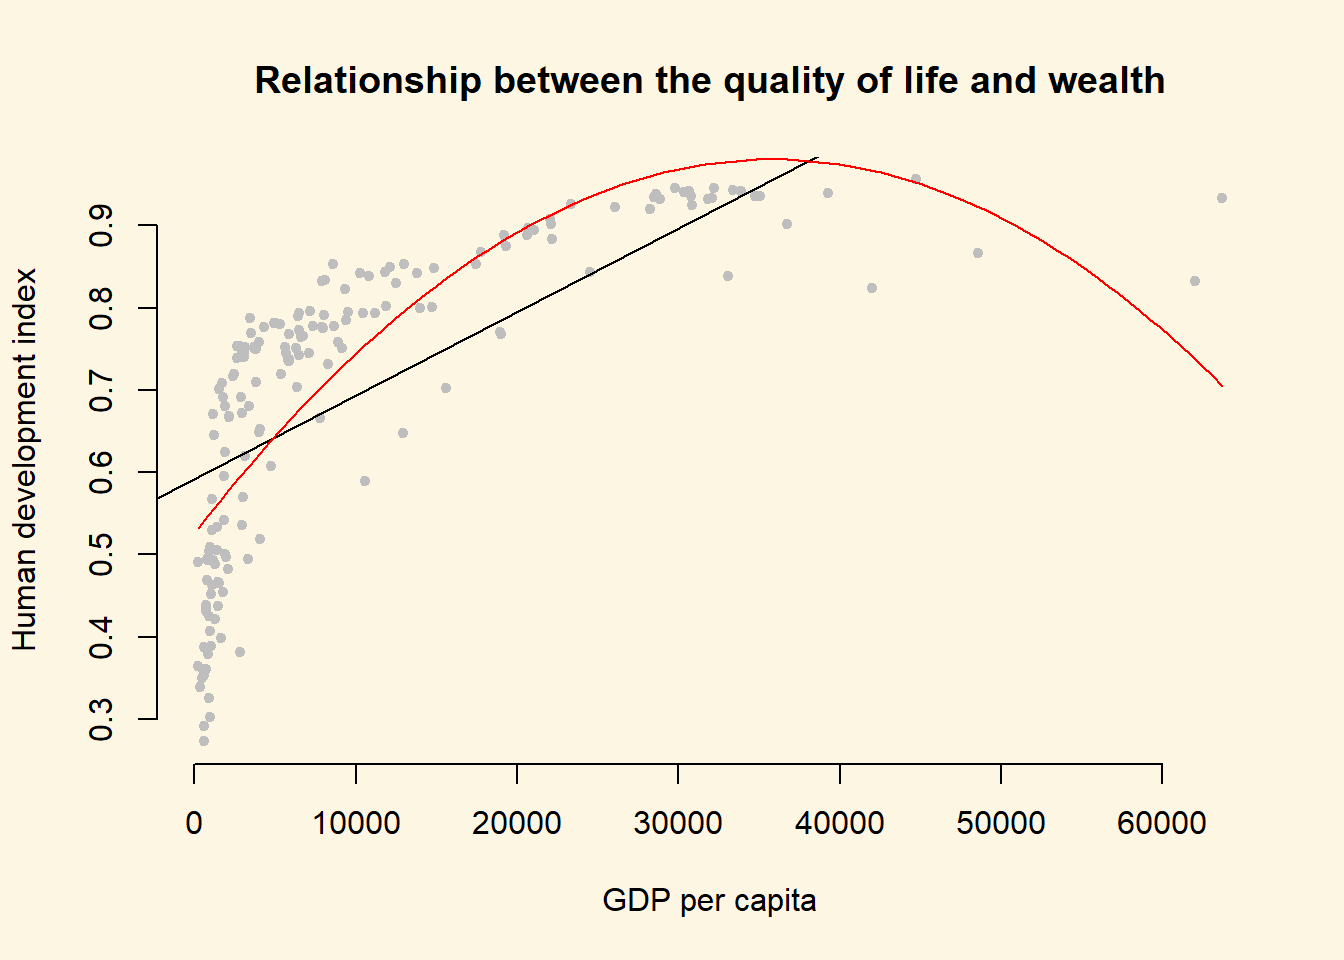
\includegraphics{suffolk2019_files/figure-latex/unnamed-chunk-180-1.pdf}

We could go further than this quadratic specification, and instead estimate a \texttt{cubic.model} with GDP/capita raised to the power of three. Do this now and present your results visually.

Estimate cubic model

\begin{Shaded}
\begin{Highlighting}[]
\NormalTok{cubic.model <-}\StringTok{ }\KeywordTok{lm}\NormalTok{(human_development }\OperatorTok{~}\StringTok{ }\KeywordTok{poly}\NormalTok{(gdp_capita, }\DecValTok{3}\NormalTok{), }\DataTypeTok{data =}\NormalTok{ world_data)}
\end{Highlighting}
\end{Shaded}

We predict the outcome (human development index) for each of the 100 GDP levels

\begin{Shaded}
\begin{Highlighting}[]
\NormalTok{y_hat2 <-}\StringTok{ }\KeywordTok{predict}\NormalTok{(cubic.model, }\DataTypeTok{newdata =}\NormalTok{ x)}
\end{Highlighting}
\end{Shaded}

Next, we plot the linear and quadratic models

\begin{Shaded}
\begin{Highlighting}[]
\KeywordTok{plot}\NormalTok{(}
  \DataTypeTok{x =}\NormalTok{ world_data}\OperatorTok{$}\NormalTok{gdp_capita,}
  \DataTypeTok{y =}\NormalTok{ world_data}\OperatorTok{$}\NormalTok{human_development,}
  \DataTypeTok{data =}\NormalTok{ world_data,}
  \DataTypeTok{pch =} \DecValTok{20}\NormalTok{,}
  \DataTypeTok{frame.plot =} \OtherTok{FALSE}\NormalTok{,}
  \DataTypeTok{col =} \StringTok{"grey"}\NormalTok{,}
  \DataTypeTok{main =} \StringTok{"Relationship between the quality of life and wealth"}\NormalTok{,}
  \DataTypeTok{ylab =} \StringTok{"Human development index"}\NormalTok{,}
  \DataTypeTok{xlab =} \StringTok{"GDP per capita"}
\NormalTok{  )}
\end{Highlighting}
\end{Shaded}

\begin{verbatim}
Warning in plot.window(...): "data" is not a graphical parameter
\end{verbatim}

\begin{verbatim}
Warning in plot.xy(xy, type, ...): "data" is not a graphical parameter
\end{verbatim}

\begin{verbatim}
Warning in axis(side = side, at = at, labels = labels, ...): "data" is not
a graphical parameter

Warning in axis(side = side, at = at, labels = labels, ...): "data" is not
a graphical parameter
\end{verbatim}

\begin{verbatim}
Warning in title(...): "data" is not a graphical parameter
\end{verbatim}

\begin{Shaded}
\begin{Highlighting}[]
\CommentTok{# the linear model}
\KeywordTok{abline}\NormalTok{(linear.model, }\DataTypeTok{col =} \StringTok{"black"}\NormalTok{)}

\CommentTok{# quadratic model}
\KeywordTok{lines}\NormalTok{(}\DataTypeTok{x =}\NormalTok{ gdp_seq, }\DataTypeTok{y =}\NormalTok{ y_hat, }\DataTypeTok{col =} \StringTok{"red"}\NormalTok{)}

\CommentTok{# cubic model}
\KeywordTok{lines}\NormalTok{(}\DataTypeTok{x =}\NormalTok{ gdp_seq, }\DataTypeTok{y =}\NormalTok{ y_hat2, }\DataTypeTok{col =} \StringTok{"green"}\NormalTok{)}
\end{Highlighting}
\end{Shaded}

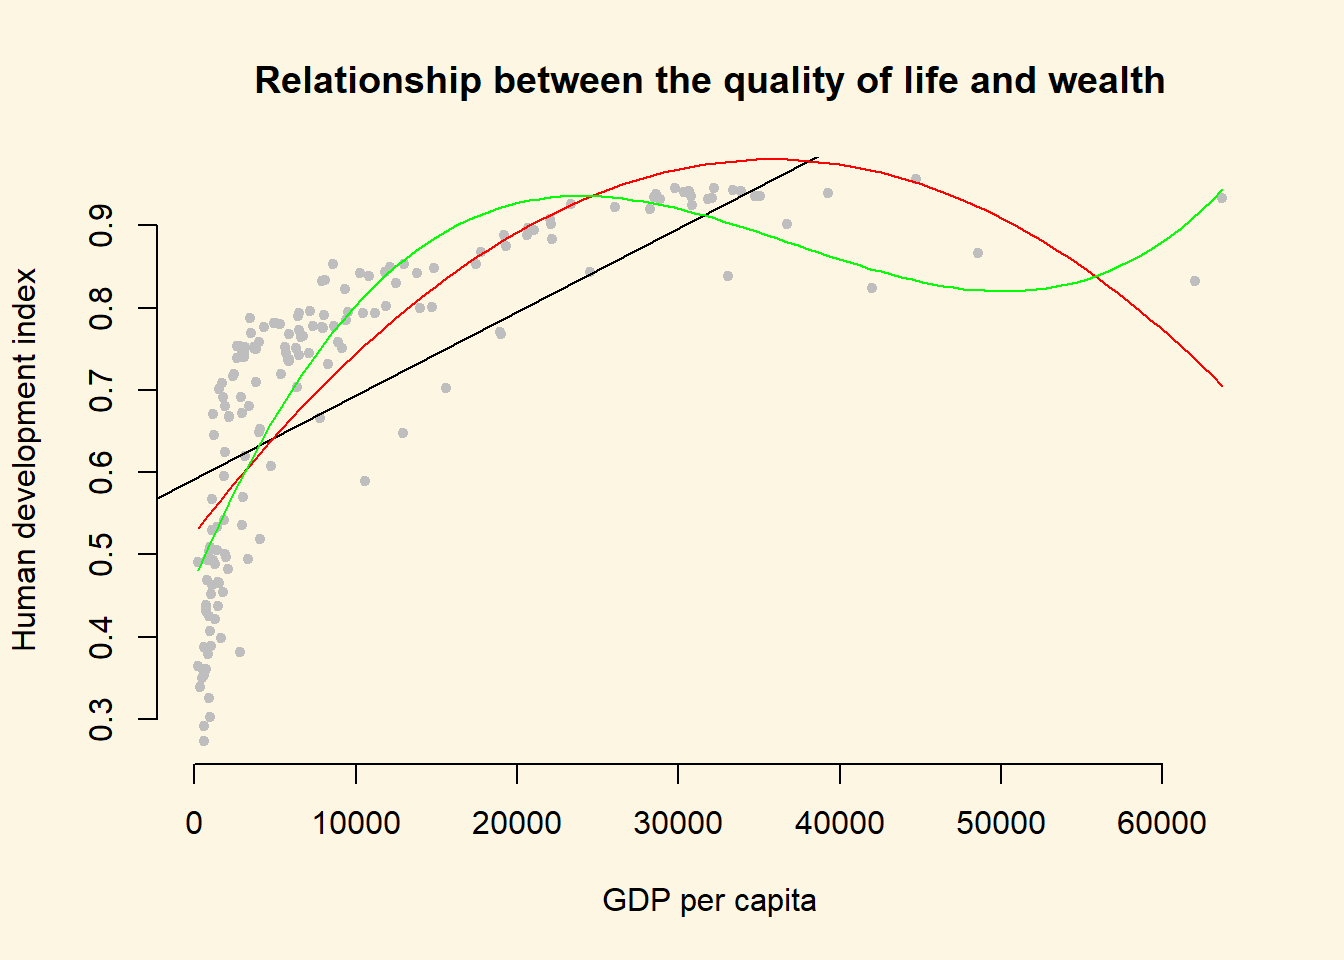
\includegraphics{suffolk2019_files/figure-latex/unnamed-chunk-183-1.pdf}

The cubic model provides a similar story to the quadratic model (the relationship between GDP/capita and HDI is steep at first, and then flatter at the higher levels of GDP/captia), but it looks somewhat strange, particularly at the higher levels of GDP/capita. In particular, it seems that the few extreme X values are causing a strange shape: the cubic is being wagged around by its tail. This is a common problem with polynomial regression models, and so we will now consider an alternative.

\hypertarget{log-transformations}{%
\paragraph{Log-transformations}\label{log-transformations}}

Many non-linear relationships actually do look linear on the log scale. We can illustrate this by taking the natural logarithm of GDP/captia and plot the relationship between quality of life and our transformed GDP variable.

Note: Some of you will remember from your school calculators that you have an ln button and a log button where ln takes the natural logarithm and log takes the logarithm with base 10. The natural logarithm represents relations that occur frequently in the world and R takes the natural logarithm with the \texttt{log()} function by default.

Below, we plot the same plot from before but we wrap \texttt{gdp\_capita} in the \texttt{log()} function which log-transforms the variable.

\begin{Shaded}
\begin{Highlighting}[]
\KeywordTok{plot}\NormalTok{(}
  \DataTypeTok{x =} \KeywordTok{log}\NormalTok{(world_data}\OperatorTok{$}\NormalTok{gdp_capita),}
  \DataTypeTok{y =}\NormalTok{ world_data}\OperatorTok{$}\NormalTok{human_development,}
  \DataTypeTok{data =}\NormalTok{ world_data,}
  \DataTypeTok{pch =} \DecValTok{20}\NormalTok{,}
  \DataTypeTok{frame.plot =} \OtherTok{FALSE}\NormalTok{,}
  \DataTypeTok{col =} \StringTok{"grey"}\NormalTok{,}
  \DataTypeTok{main =} \StringTok{"Relationship between the quality of life and wealth on the log scale"}\NormalTok{,}
  \DataTypeTok{ylab =} \StringTok{"Human development index"}\NormalTok{,}
  \DataTypeTok{xlab =} \StringTok{"Logged gdp/capita"}
\NormalTok{  )}
\end{Highlighting}
\end{Shaded}

\begin{verbatim}
Warning in plot.window(...): "data" is not a graphical parameter
\end{verbatim}

\begin{verbatim}
Warning in plot.xy(xy, type, ...): "data" is not a graphical parameter
\end{verbatim}

\begin{verbatim}
Warning in axis(side = side, at = at, labels = labels, ...): "data" is not
a graphical parameter

Warning in axis(side = side, at = at, labels = labels, ...): "data" is not
a graphical parameter
\end{verbatim}

\begin{verbatim}
Warning in title(...): "data" is not a graphical parameter
\end{verbatim}

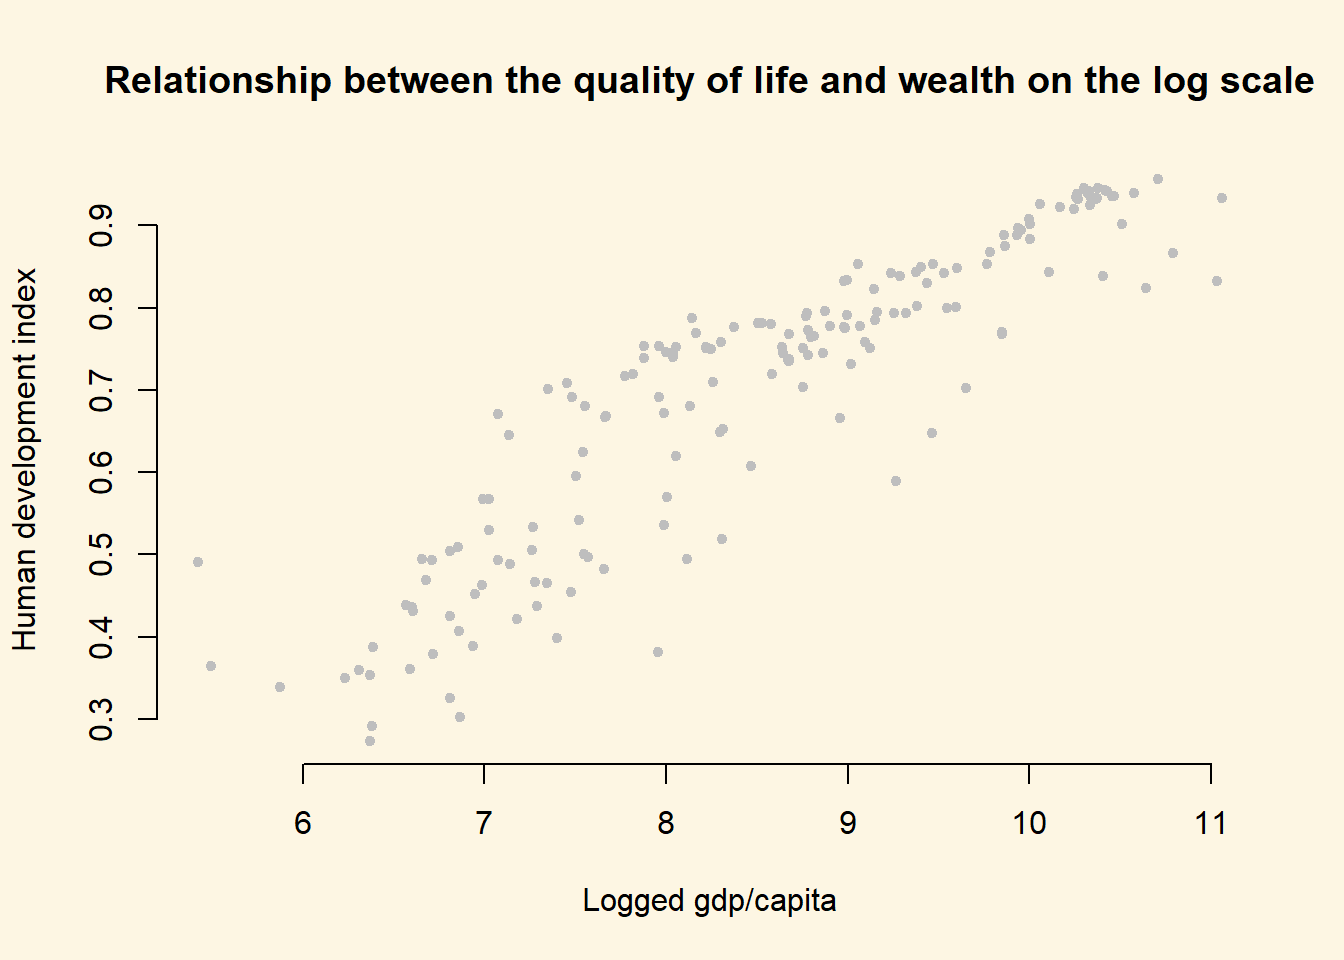
\includegraphics{suffolk2019_files/figure-latex/unnamed-chunk-184-1.pdf}

As you can see, the relationship now looks much closer to linear and we get the best fit to the data (as measured by adjusted \(R^2\)) if we run our model with log-transformed gdp.

\begin{Shaded}
\begin{Highlighting}[]
\NormalTok{log.model <-}\StringTok{ }\KeywordTok{lm}\NormalTok{(human_development }\OperatorTok{~}\StringTok{ }\KeywordTok{log}\NormalTok{(gdp_capita), }\DataTypeTok{data =}\NormalTok{ world_data)}
\end{Highlighting}
\end{Shaded}

Let's check our model

\begin{Shaded}
\begin{Highlighting}[]
\KeywordTok{screenreg}\NormalTok{(}
  \KeywordTok{list}\NormalTok{(linear.model, quadratic.model, cubic.model, log.model),}
  \DataTypeTok{custom.model.names =} \KeywordTok{c}\NormalTok{(}\StringTok{"Linear Model"}\NormalTok{, }\StringTok{"Quadratic Model"}\NormalTok{, }\StringTok{"Cubic Model"}\NormalTok{, }\StringTok{"Log Model"}\NormalTok{)}
\NormalTok{)}
\end{Highlighting}
\end{Shaded}

\begin{verbatim}

=====================================================================================
                               Linear Model  Quadratic Model  Cubic Model  Log Model 
-------------------------------------------------------------------------------------
(Intercept)                      0.59 ***      0.70 ***         0.70 ***    -0.36 ***
                                (0.01)        (0.01)           (0.01)       (0.04)   
gdp_capita                       0.00 ***                                            
                                (0.00)                                               
poly(gdp_capita, degree = 2)1                  1.66 ***                              
                                              (0.10)                                 
poly(gdp_capita, degree = 2)2                 -1.00 ***                              
                                              (0.10)                                 
poly(gdp_capita, 3)1                                            1.66 ***             
                                                               (0.09)                
poly(gdp_capita, 3)2                                           -1.00 ***             
                                                               (0.09)                
poly(gdp_capita, 3)3                                            0.65 ***             
                                                               (0.09)                
log(gdp_capita)                                                              0.12 ***
                                                                            (0.00)   
-------------------------------------------------------------------------------------
R^2                              0.49          0.67             0.74         0.81    
Adj. R^2                         0.49          0.66             0.74         0.81    
Num. obs.                      172           172              172          172       
RMSE                             0.13          0.10             0.09         0.08    
=====================================================================================
*** p < 0.001, ** p < 0.01, * p < 0.05
\end{verbatim}

Polynomials can be useful for modelling non-linearities. However, for each additional polynomial term we add, we also add an additional parameter that needs to be estimated. This reduces the degrees of freedom of the model. If we can get a linear relationship on the log scale, one advantage is that we use the same number of parameters as in the original linear model.

Furthermore, we gain interpretability. The relationship is linear on the log scale of gdp/capita. This means we can interpret the effect of gdp/captia as: For an increase of gdp/captia by one percent, the quality of life increases by \(\frac{\hat{\beta}}{100} = \frac{0.12}{100}\) points on average. The effect is very large because \texttt{human\_development} only varies from \(0\) to \(1\).

The adjusted \(R^2\) also suggests that the log model provides the best fit to the data. To illustrate that this is the case, we return to our plot and show the model fit graphically.

Get the fitted values for the log model.

\begin{Shaded}
\begin{Highlighting}[]
\NormalTok{y_hat3 <-}\StringTok{ }\KeywordTok{predict}\NormalTok{(log.model, }\DataTypeTok{newdata =}\NormalTok{ x)}
\end{Highlighting}
\end{Shaded}

Create a plot showing the fitted values

\begin{Shaded}
\begin{Highlighting}[]
\KeywordTok{plot}\NormalTok{(}
  \DataTypeTok{x =}\NormalTok{ world_data}\OperatorTok{$}\NormalTok{gdp_capita,}
  \DataTypeTok{y =}\NormalTok{ world_data}\OperatorTok{$}\NormalTok{human_development,}
  \DataTypeTok{data =}\NormalTok{ world_data,}
  \DataTypeTok{pch =} \DecValTok{20}\NormalTok{,}
  \DataTypeTok{frame.plot =} \OtherTok{FALSE}\NormalTok{,}
  \DataTypeTok{col =} \StringTok{"grey"}\NormalTok{,}
  \DataTypeTok{main =} \StringTok{"Relationship between the quality of life and wealth"}\NormalTok{,}
  \DataTypeTok{ylab =} \StringTok{"Human development index"}\NormalTok{,}
  \DataTypeTok{xlab =} \StringTok{"GDP per capita"}
\NormalTok{  )}
\end{Highlighting}
\end{Shaded}

\begin{verbatim}
Warning in plot.window(...): "data" is not a graphical parameter
\end{verbatim}

\begin{verbatim}
Warning in plot.xy(xy, type, ...): "data" is not a graphical parameter
\end{verbatim}

\begin{verbatim}
Warning in axis(side = side, at = at, labels = labels, ...): "data" is not
a graphical parameter

Warning in axis(side = side, at = at, labels = labels, ...): "data" is not
a graphical parameter
\end{verbatim}

\begin{verbatim}
Warning in title(...): "data" is not a graphical parameter
\end{verbatim}

\begin{Shaded}
\begin{Highlighting}[]
\CommentTok{# Linear model}
\KeywordTok{abline}\NormalTok{(linear.model, }\DataTypeTok{col =} \StringTok{"black"}\NormalTok{)}

\CommentTok{# Quadratic model}
\KeywordTok{lines}\NormalTok{(}\DataTypeTok{x =}\NormalTok{ gdp_seq, }\DataTypeTok{y =}\NormalTok{ y_hat, }\DataTypeTok{col =} \StringTok{"red"}\NormalTok{)}

\CommentTok{# Cubic model}
\KeywordTok{lines}\NormalTok{(}\DataTypeTok{x =}\NormalTok{ gdp_seq, }\DataTypeTok{y =}\NormalTok{ y_hat2, }\DataTypeTok{col =} \StringTok{"green"}\NormalTok{)}

\CommentTok{# Log model}
\KeywordTok{lines}\NormalTok{(}\DataTypeTok{x =}\NormalTok{ gdp_seq, }\DataTypeTok{y =}\NormalTok{ y_hat3, }\DataTypeTok{col =} \StringTok{"blue"}\NormalTok{)}

\CommentTok{# Add a legend}
\KeywordTok{legend}\NormalTok{(}\StringTok{"bottomright"}\NormalTok{, }
       \DataTypeTok{legend =} \KeywordTok{c}\NormalTok{(}\StringTok{"Linear"}\NormalTok{, }\StringTok{"Quadratic"}\NormalTok{, }\StringTok{"Cubic"}\NormalTok{, }\StringTok{"Log"}\NormalTok{), }
       \DataTypeTok{lty =} \DecValTok{1}\NormalTok{, }
       \DataTypeTok{col =} \KeywordTok{c}\NormalTok{(}\StringTok{"black"}\NormalTok{, }\StringTok{"red"}\NormalTok{, }\StringTok{"green"}\NormalTok{, }\StringTok{"blue"}\NormalTok{) }
\NormalTok{)}
\end{Highlighting}
\end{Shaded}

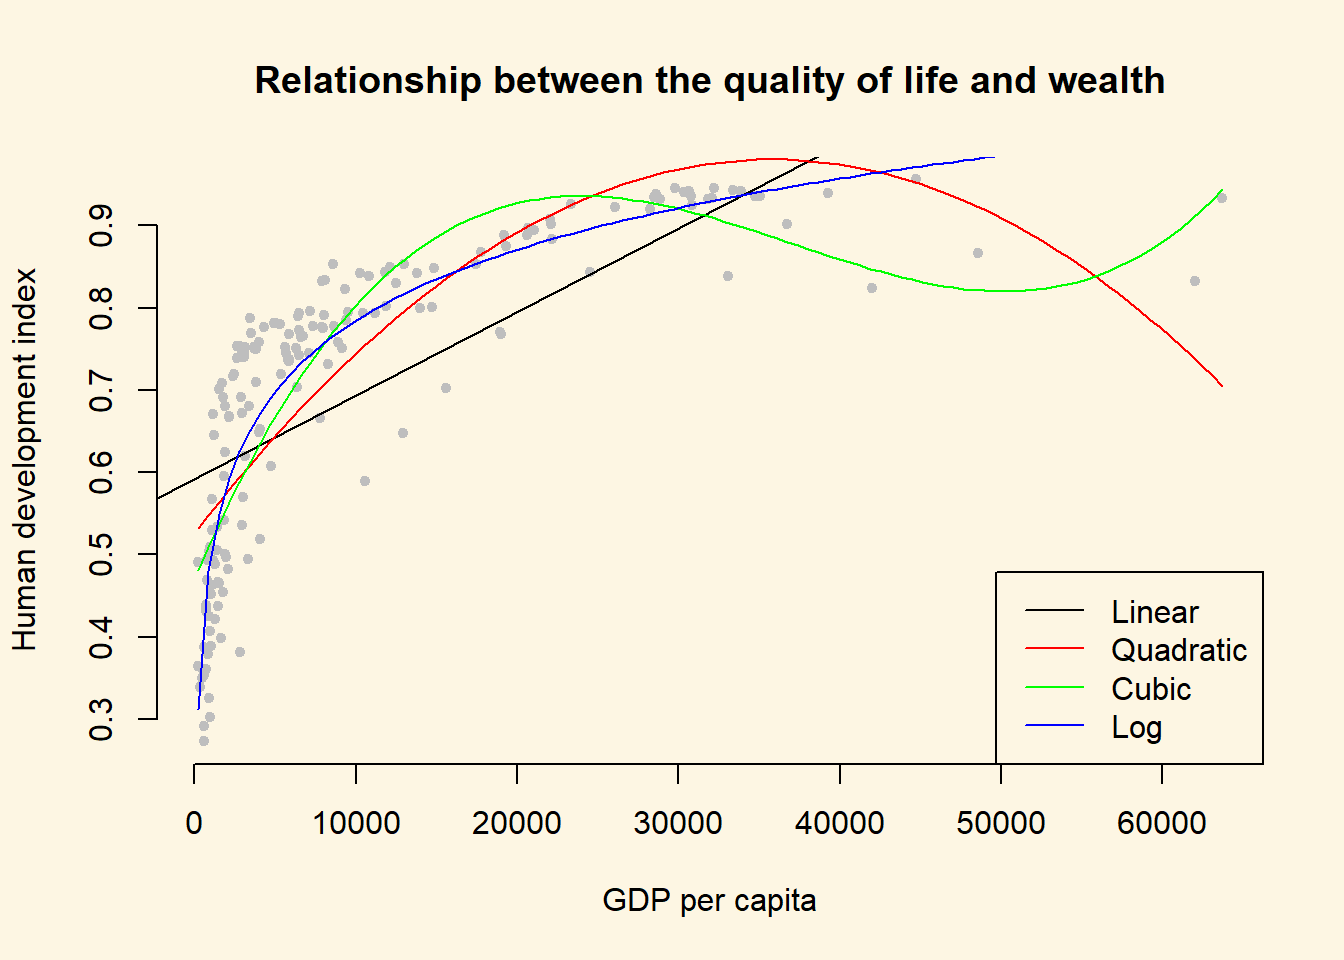
\includegraphics{suffolk2019_files/figure-latex/unnamed-chunk-188-1.pdf}

The blue line shows the log-transformed model. It clearly fits the data best.

\hypertarget{prediction-and-assessing-prediction-accuracy}{%
\section{Prediction and assessing prediction accuracy}\label{prediction-and-assessing-prediction-accuracy}}

\hypertarget{seminar-8}{%
\subsection{Seminar}\label{seminar-8}}

Will be uploaded tomorrow


\end{document}
